\section{Limitations of Existing Approaches}
\label{sec:midsurfcelljoin:existingapproach}

\replaced{Review of the}{After analyzing various} past approaches \replaced{indicate}{it can be concluded} that, Face Pairing (also known as Midsurface Abstraction) is one of the most representative approaches for midsurface generation~\cite{Sheen2008}. 
\todo[inline]{Telephone comment: Explain face pairing midsurface generation approach with figure, label face pairs, how midsurface is generated. [DONE]}
In the Face Pairing approach, faces opposite each other are identified by ray-firing method and are grouped as face-pairs \cite{Rezayat1996}.

\todo{Review comment: Can you enlarge this and show separately, to show master, slave, ray fired. [ADDED SEPARATE ENLARGED PICTURE. MASTER SLAVE IN THE SCHEMATICS LATER]}

%%\bigskip

	\begin{figure}[h!]
	\centering 
	%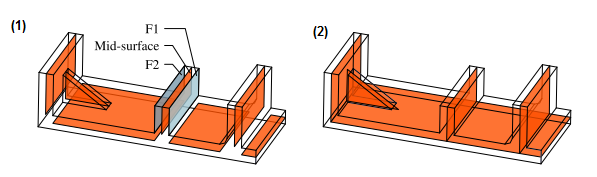
\includegraphics[width=0.85\linewidth]{../Common/images/facepairing}
	\subfloat[Full model view]{\label{fig:midsurfcelljoin:facepairmids}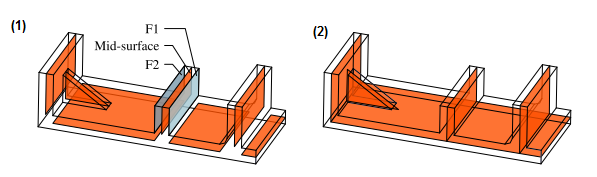
\includegraphics[width=0.72\linewidth,valign=t]{../Common/images/facepairing}} \quad
	\subfloat[Magnified view]{\label{fig:midsurfcelljoin:midsjoining}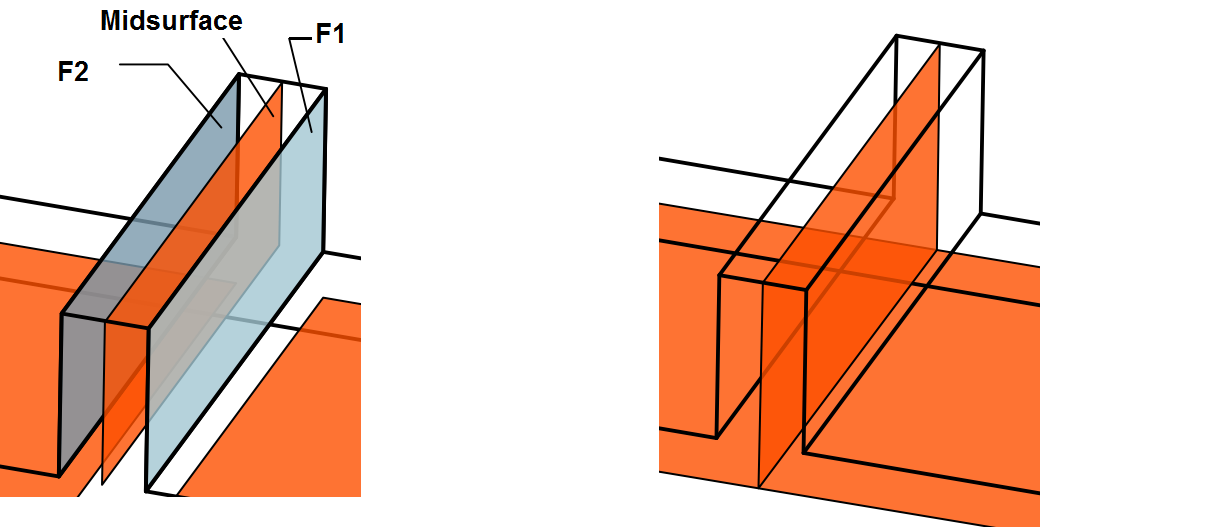
\includegraphics[width=0.62\linewidth,valign=t]{../Common/images/facepairingamplified}}
	\caption{Face Pairing Approach (Source: Boussuge \cite{Boussuge2014})}
	\label{fig:midsurfcelljoin:facepairing}
	\end{figure}

%%\bigskip

Figure~\ref{fig:midsurfcelljoin:facepairing} shows an example model in two stages of midsurface computation. Figure~\ref{fig:midsurfcelljoin:facepairmids}(1) shows midsurface patches whereas Figure~\ref{fig:midsurfcelljoin:facepairmids}(2) shows them joined. Figure~\ref{fig:midsurfcelljoin:midsjoining} shows magnified view of the same model. In Figure \ref{fig:midsurfcelljoin:facepairmids}(1), one of the face-pairs is marked for an example, as $F_1-F_2$. The face from which a ray is fired is called as ``master face'' ($F_1$) and the target which got identified as the opposite face, is called as the ``slave face'' ($F_2$). Figure~\ref{fig:midsurfcelljoin:facepairmids}(2) shows the patches extended or trimmed, brought at a common edge and then joined to form a well-connected midsurface. 
\todo{Review comment: How midsurface is generated. [ADDED]}
 The face pairing approach scores over the other approaches such as MAT, as it is intuitive and does not need post-processing to remove extra branches \cite{Rezayat1996}. It is widely researched and used in academic as well as commercial CAD-CAE systems.

\todo[inline]{Review comment: May be you could give 2-3 lines before you start the section. [DONE AS BELOW]}

\replaced{In-spite of its wide usage, the face pairing approach however has two critical issues, namely, Face Pairs Detection and Midsurface Patch Joining. These issues aggravate as the complexity of the model increases and result in various errors in the output midsuface. These are explained in the following subsections.}{Two of the critical problems, which are hindrance to computing a quality midsurface, are elaborated below, along with the proposed approaches to tackle them. }\deleted{ such as missing surfaces, gaps, overlaps, etc. Correcting these errors is tedious and often manually laborious task ranging from hours to days. So, addressing these critical issues is of utmost importance in getting a quality midsurface.}
	
\subsection{Face Pairs Detection Problem}  \label{sec:midsurfcelljoin:facepairdetection}
%A widely used Face pairing process, a ray is fired from a seed face in the given CAD model. The nearest face that is hit by the ray and  which is within given threshold thickness distance, is the target and is selected to form the face pair along with the seed face. The process repeats with another faces as the seed face, till all the remaining faces are processed. The output face-pairs list is sent for mdisurface patch generation.

\todo{Reviewer comment: Explain only face pairing problem. Do not give any solution here. [DONE]}

For real-life complex CAD models detecting opposite faces is challenging \cite{Woo2014, Zhu2016}. 
%\deleted{As seen in Section \ref{sec:midsurfcelljoin:existingapproach}, a}A face pair is formed by finding opposite faces. A ray from a face (called `master') fired which hits other faces in its direction. Face hit by the ray within a threshold distance (equivalent to the sheet metal thickness) are the opposite faces (called `slaves'). One master and multiple slave faces form a face pair. Finding face pairs in a complex model is challenging and error-prone. 
Some of such scenarios are described below:

%%\bigskip


\begin{figure}[!h]%[!h]
\centering     %%% not \center
\subfloat[Missing target]{\label{fig:midsurfcelljoin:missingtarget}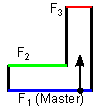
\includegraphics[width=0.21\linewidth,valign=t]{../Common/images/missingtarget.pdf}} \quad
\subfloat[Multiple targets]{\label{fig:midsurfcelljoin:multipletargets}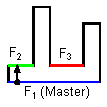
\includegraphics[width=0.21\linewidth,valign=t]{../Common/images/multipletargets.pdf}} \quad
\subfloat[Angled targets]{\label{fig:midsurfcelljoin:angledtargets}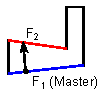
\includegraphics[width=0.21\linewidth,valign=t]{../Common/images/angledtargets.pdf}}
\caption{Problems in Identification of Face Pairs} 
\label{fig:midsurfcelljoin:facepairingproblems}
\end{figure}

%%\bigskip


\todo{Reviewer comment: Label master and slave. [LABELED MASTER BUT NOT SLAVE BECAUSE IT HAS NOT BEEN SELECTED]}

\begin{itemize}[noitemsep,topsep=2pt,parsep=2pt,partopsep=2pt]
\item \textbf{Missing target}: If a face is not within threshold distance, or not in the direction of the ray-fire from the master, it fails to get detected as the slave. In Figure \ref{fig:midsurfcelljoin:missingtarget}, $F_1$ is the master face from which a ray is fired (shown by an arrow). It does not hit $F_2$\deleted{as it does not in the ray firing direction}, so it does not get qualified as the slave face. The ray hits $F_3$ but it is too far way, so fails the threshold distance criteria, thus $F_3$ also does not get qualified as the slave. So, incorrect choice of the location from which ray is fired, misses as the otherwise qualified slave face, such as $F_2$ in this case.
\item \textbf{Multiple targets}: There could be multiple candidate salve faces for a single master face, approximately at similar distances, but, either due to tolerance issues or due to location from which the ray is fired, only one of them gets selected, discarding other equally eligible candidate slave faces. In Figure \ref{fig:midsurfcelljoin:multipletargets}, master face $F_1$ correctly identifies $F_2$ but does not find $F_3$ as the ray was not fired from the location which would find it. So $F_3$ does not get added to the same face pair as with $F_2$. Ideally a face pair with $F_1$ as master face and $F_2 \& F_3$ as slave faces should have got formed.
\item \textbf{Angled targets}: In case of variable thickness shapes, distance between master and slave faces vary, making it challenging to decide appropriate slave face. Figure \ref{fig:midsurfcelljoin:angledtargets} shows that $F_1$ is not able to pair up with $F_2$ due to being farther away from the allowed distance threshold.
\item \textbf{Non-planar targets}: Non planar geometries such as free-form surfaces also pose problems in calculation of distances and finding slave faces \cite{Zhu2016}.
\end{itemize}

Such undetected or inappropriately detected face pairs do not create appropriate midsurface patches thus leaving gaps in the overall midsurface output. Next section discusses problems encountered in joining the midsurface patches.

%%Face pairs, in an abstracted way, decompose the whole model into sub-volumes. Each sub-volume creates its own midsurface patch which, later, are ``sewed'' together. Detecting face-pairs are extremely challenging task, especially for complex shapes and is prone to failures. Instead of working on the final shape, this work tests if features can be used to alleviate this problem (Hypothesis \ref{hyp:features}).

%%In the feature based CAD model, at each feature step, a tool-body/sub-volume is created and booleaned to the existing model.  Instead of detecting face pairs in the final solid,  feature information, at each step, can be leveraged to compute the midsurface patch for it's corresponding sub-volume. But, writing the midsurface computation logic for each of the features-types would be a humongous and error-prone task.  This work solves this problem by abstracting/generalizing these individual feature types into a generic form and then compute midsurface patches for just the generic type (Hypothesis \ref{hyp:Abstraction}). Feature abstraction called $\mathcal{ABLE}$ has been proposed to generalize the form features into a generic ``Loft'' feature having profile(s) and a guide curve. Midsurface patch can then be computed by sweeping midcurve of the profile(s) along the guide curve (Section \ref{sec:midsurfcelljoin:scell}) (\cite{YogeshIITG2014}).

%A feature generalization framework called $\mathcal{ABLE}$ ({\bf A}ffine transformations-{\bf B}ooleans-{\bf E}ntities-{\bf L}ofts), shows that a majority of the widely-used form-features can be represented as the ``Sweep'' feature (Figure \ref{fig:midsurfcelljoin:loftschematic}, Sweep, being a special case of Loft, both terms are used interchangeably in this paper), having inputs as a profile and  a guide curve. Figure \ref{fig:midsurfcelljoin:extrudeschematic} shows how the generic Sweep manifests into Extrude and Revolve features, where as Figure \ref{fig:midsurfcelljoin:primitivesschematic} shows further manifestations into primitive shapes. 
%
%
%\begin{figure}[!h]%[!h]
%\centering     %%% not \center
%\subfloat[Generic Loft/Sweep]{\label{fig:midsurfcelljoin:loftschematic}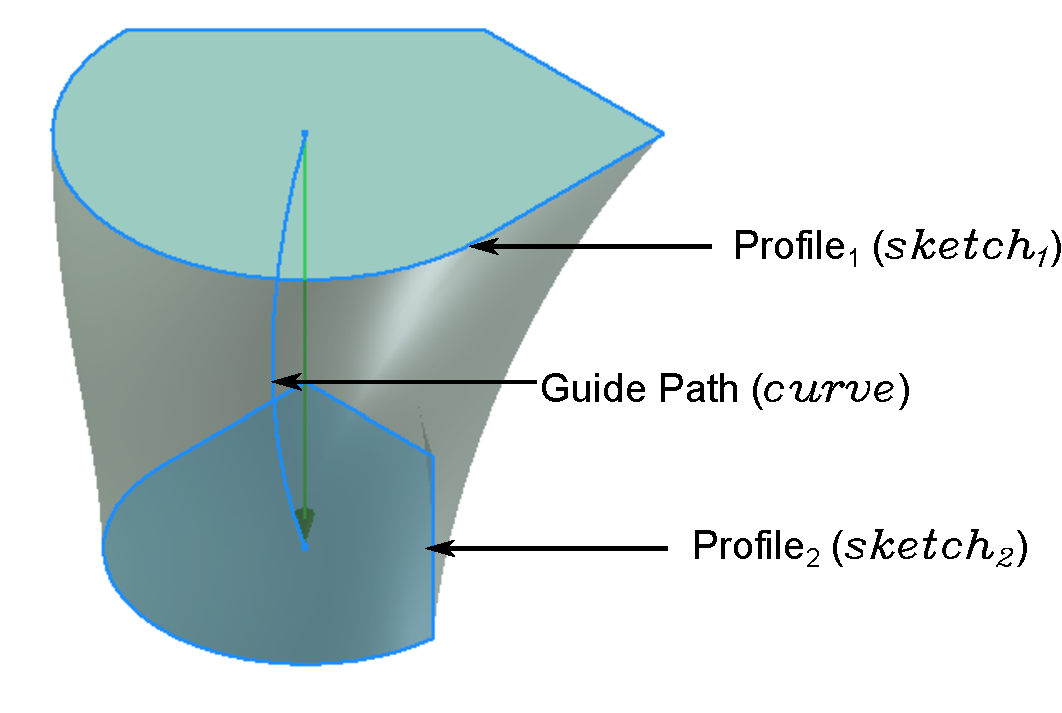
\includegraphics[width=0.4\linewidth,valign=t]{../Common/images/LoftPreview.pdf}}
%\subfloat[Extrude/Revolve as Sweep]{\label{fig:midsurfcelljoin:extrudeschematic}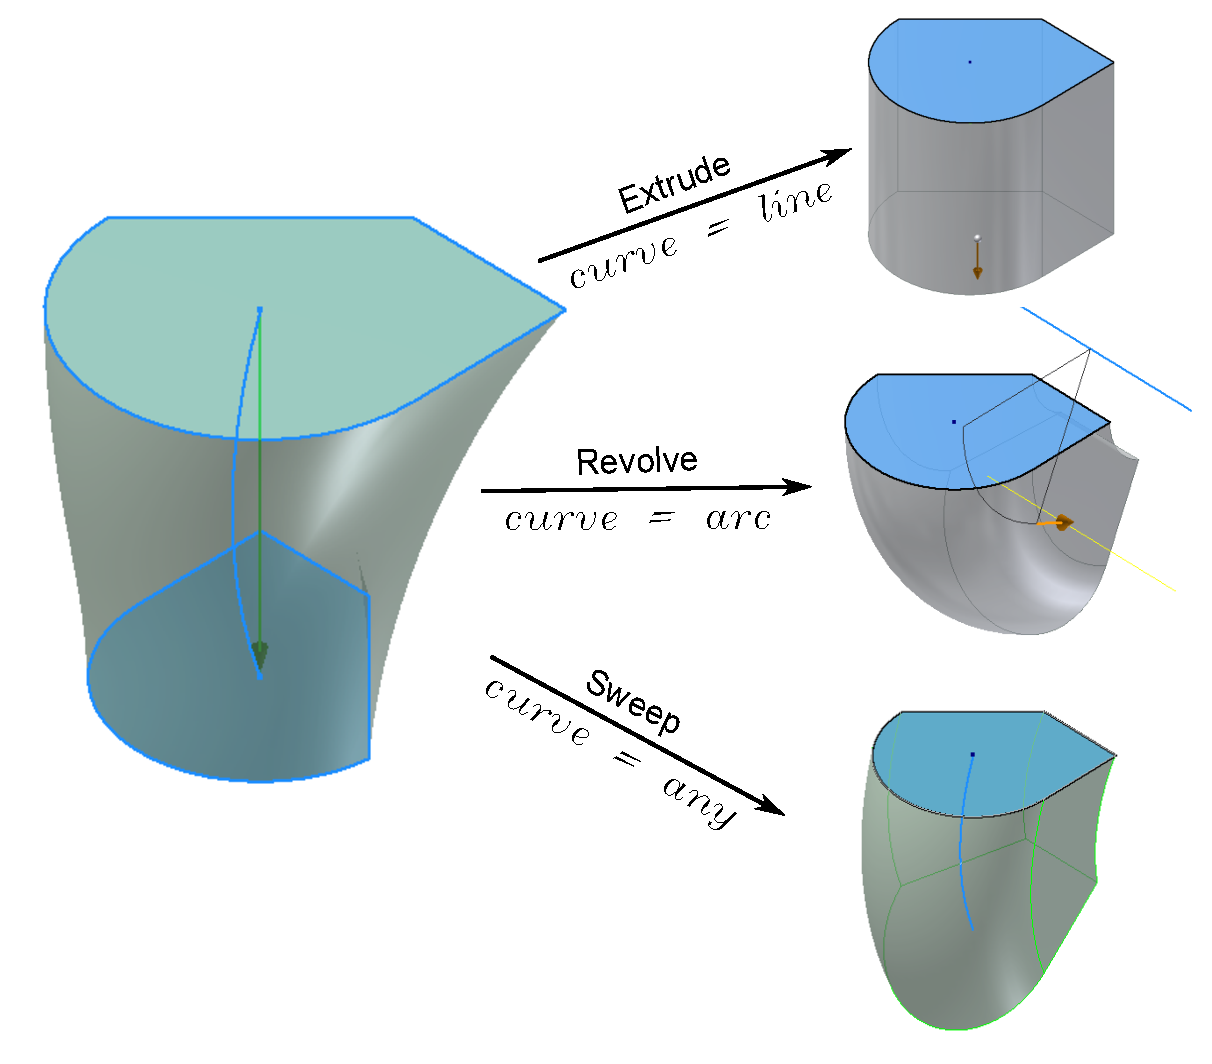
\includegraphics[width=0.31\linewidth,valign=t]{../Common/images/LoftExtrudeRevSwp.pdf}}
%\subfloat[Primitives as Extrudes]{\label{fig:midsurfcelljoin:primitivesschematic}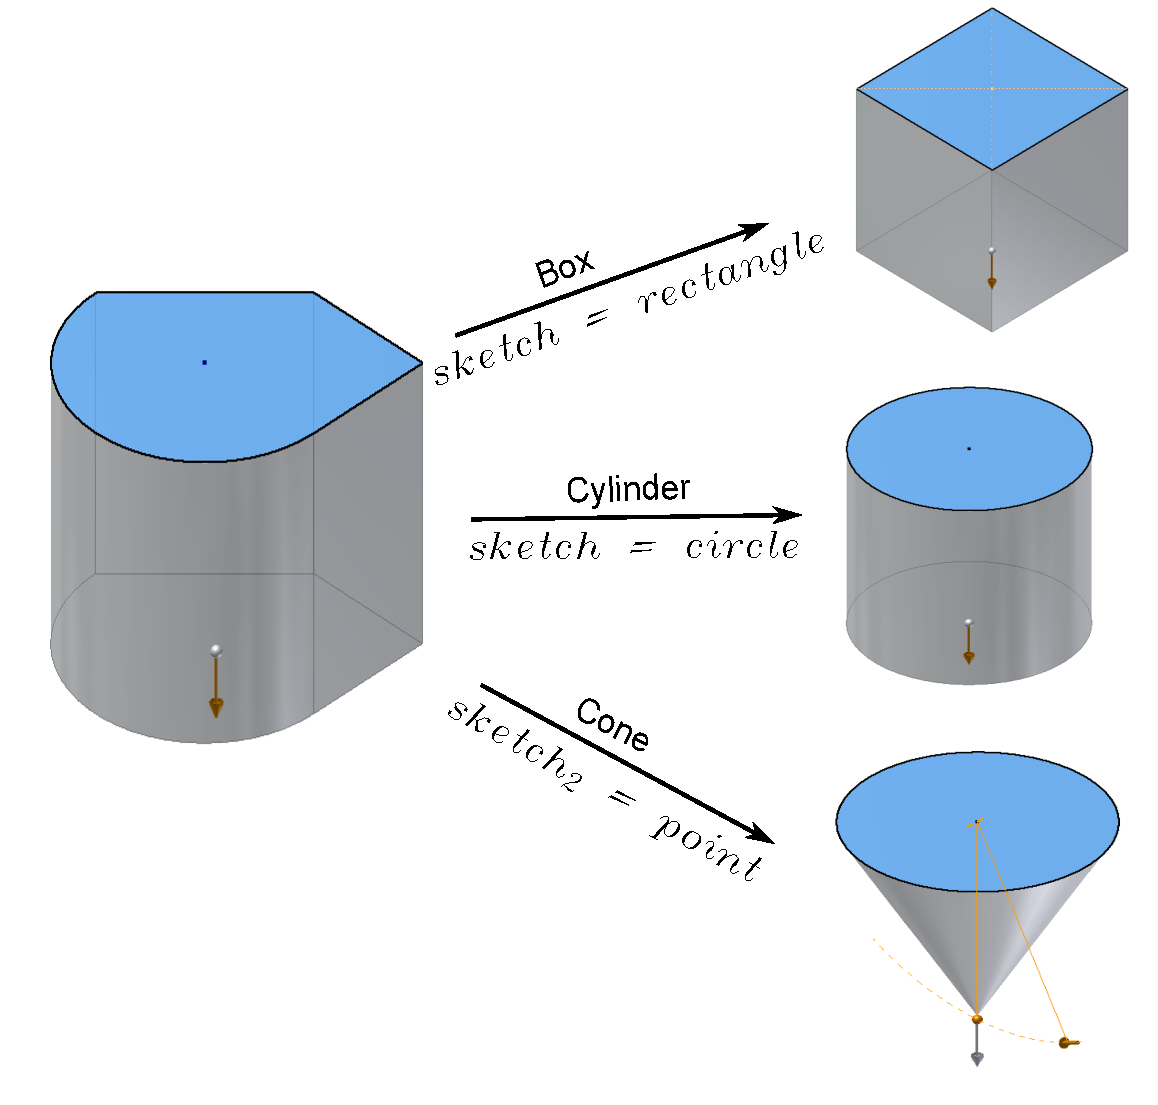
\includegraphics[width=0.28\linewidth,valign=t]{../Common/images/ExtrudeBoxCylCone.pdf}}
%\caption{Manifestation of Generic Sweep/Loft into other features (\cite{YogeshIITG2014})} %%%%%%%%% ADD  (\cite{YogeshIITG2014}) LATER
%\label{fig:midsurfcelljoin:ableschematic}
%\end{figure}
%\begin{figure}[!h]%[!h]
%\centering     %%% not \center
%\subfloat{\label{fig:midsurfcelljoin:Ubracketnormalfeatures}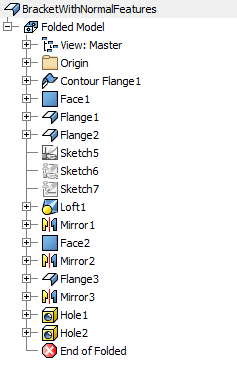
\includegraphics[width=0.25\linewidth,valign=t]{../Common/images/UBracket_normalfeatures}}
%\subfloat{\label{fig:midsurfcelljoin:Ubracketpart}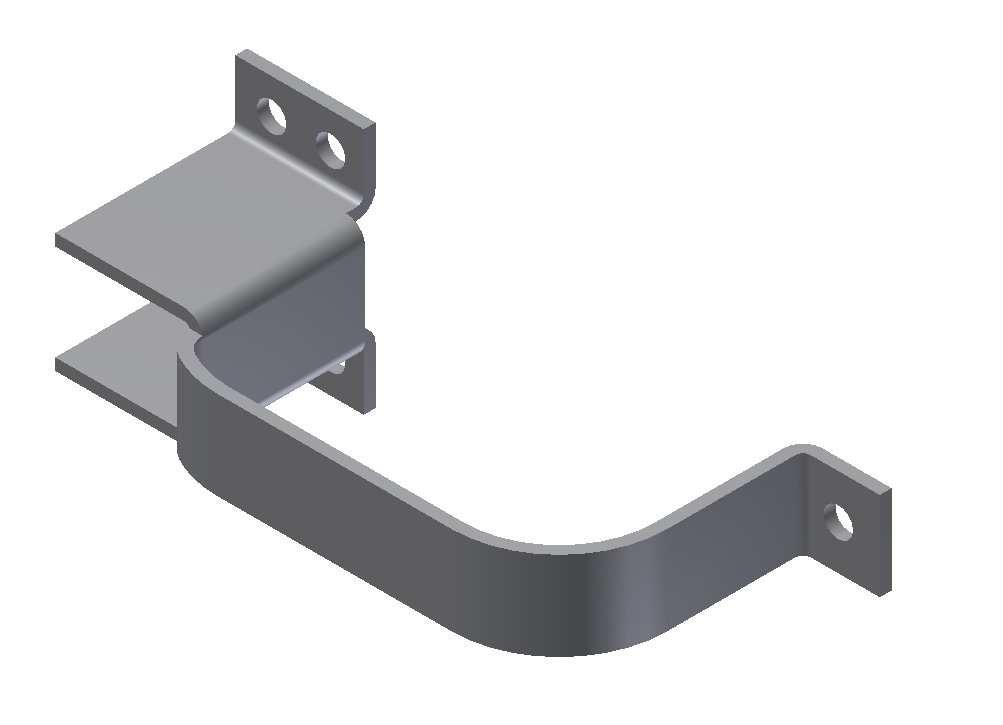
\includegraphics[width=0.45\linewidth,valign=t]{../Common/images/UBracket_part}}
%\subfloat{\label{fig:midsurfcelljoin:Ubrackettree}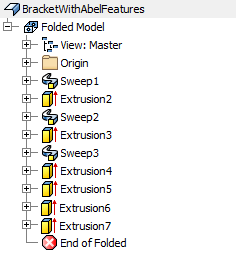
\includegraphics[width=0.25\linewidth,valign=t]{../Common/images/UBracket_abelfeatures}}
%\caption{Conversion of Normal Feature tree to $\mathcal{ABLE}$ feature Tree (\cite{YogeshIITG2014})} 
%\label{fig:midsurfcelljoin:Ubracketable}
%\end{figure}
% Figure \ref{fig:midsurfcelljoin:Ubracketable} shows how $\mathcal{ABLE}$ converts a usual feature tree to a Sweep tree (Extrude/Revolve being special cases of Sweep). By developing midsurface logic just for the ``Sweep'' feature, midsurface patches can be extracted for the majority of the models. This feature generalization, as proposed by $\mathcal{ABLE}$, thus, removes the need for doing face-pair detection and also simplifies midsurface patch computation by making it more generic and deterministic (\cite{YogeshIITG2014}).

%%Section \ref{sec:midsurfcelljoin:scell} details on how generalized features representation ($\mathcal{ABLE}$) avoids these face pairing problems. 

 
\subsection{Midsurface Patches Joining Problems} \label{sec:midsurfcelljoin:facepairinteraction}

Midsurface patches are generated from each face pair, either by offsetting the master face in the middle or by computing a surface equidistant from both, master and slave faces. As seen in Figure~\ref{fig:midsurfcelljoin:midsjoining}, they are then joined, either by extending or trimming up-to a common edge between them. Failing to compute correct extensions, trimmings, etc. result in unconnected midsurface patches.

\begin{figure}[h!]
	\centering 
	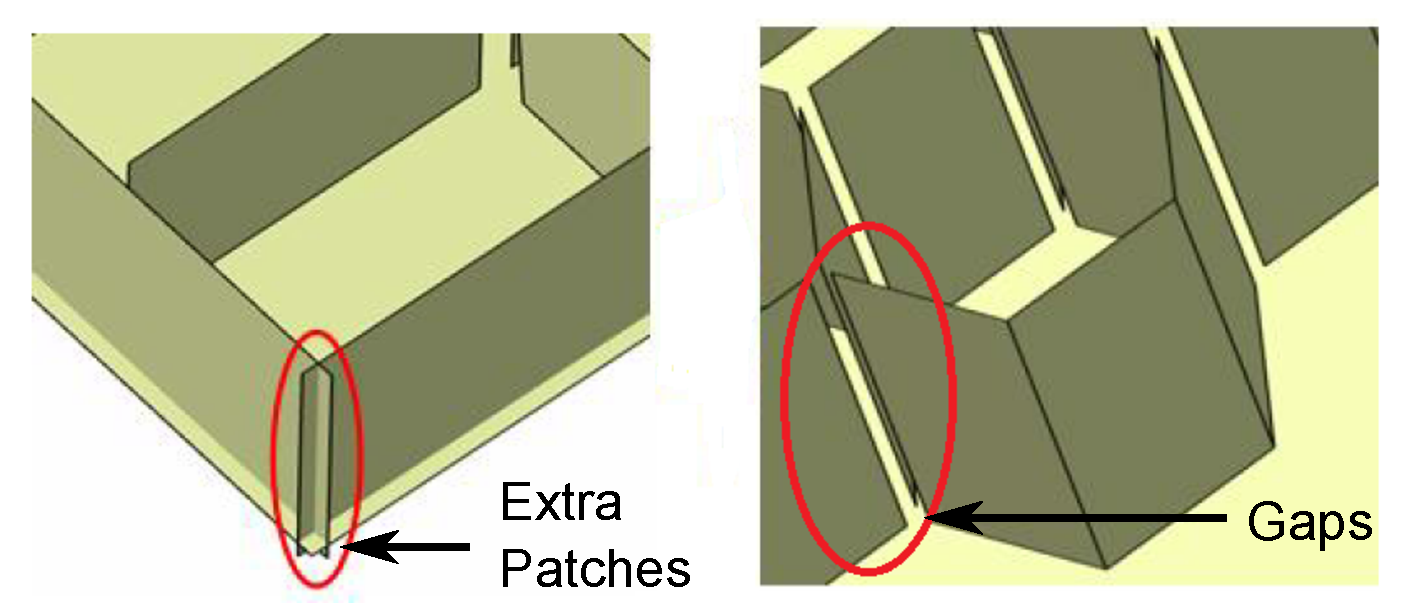
\includegraphics[width=0.62\linewidth]{../Common/images/patchjoiningproblems.pdf}
	\caption{Problems in Joining Midsurface Patches (Source: Sheen \cite{Sheen2005}) }
	\label{fig:midsurfcelljoin:patchjoiningproblems}
	\end{figure}
	
%In traditional approaches, many midsurface patches fail to get joined, resulting in gaps, overlaps, etc. to form a well connected, continuous midsurface. 
Figure \ref{fig:midsurfcelljoin:patchjoiningproblems} shows cases where the midsurface patches, either got extended too much or failed short of the common edge. 

%%%\bigskip

Basic principle of joining the midsurface patches is that they need to be connected in the same manner as their corresponding face-pairs are connected, in the input model. Detecting when to extend the midsurface patches and by what amount, also, when to trim the midsurface patches and by what amount, are complex \replaced{problems}{decisions}. These depend on various configurations in which face pairs or features (and their corresponding midsurface patches) are connected in the input model.

%%\bigskip

%\begin{table}[H]%[!h]
\begin{center}
\captionof{table}{Variety of Configurations of Interactions of Midsurfaces Patches}
%\resizebox{0.8\linewidth}{!}{
\begin{longtable}[htb]{@{}p{0.18\linewidth} p{0.25\linewidth}  p{0.25\linewidth}  p{0.25\linewidth} @{}} \toprule
{\bf Configuration} & {\bf Interaction}  & {\bf Midsurface} & {\bf Midsurface Joining Strategy} \\ \midrule  
L   &
\adjustbox{valign=t}{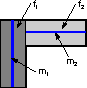
\includegraphics[width=0.8\linewidth]{../Common/images/L_interaction_part.pdf}}  &  
\adjustbox{valign=t}{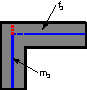
\includegraphics[width=0.8\linewidth]{../Common/images/L_interaction_midsurf.pdf}} &  
$m_2$ needs to be extended to meet $m_1$, whereas $m_1$ needs to be trimmed. 
\\ \\ \midrule

T   &
\adjustbox{valign=t}{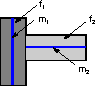
\includegraphics[width=0.9\linewidth]{../Common/images/T_interaction_part.pdf}}  &  
\adjustbox{valign=t}{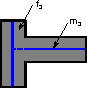
\includegraphics[width=0.8\linewidth]{../Common/images/T_interaction_midsurf.pdf}} &  
$m_2$ needs to be extended to meet $m_1$, whereas $m_1$ remains unchanged. 
\\ \\ \midrule

X  &
\adjustbox{valign=t}{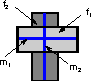
\includegraphics[width=\linewidth]{../Common/images/X_interaction_part.pdf}}  &  
\adjustbox{valign=t}{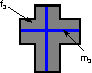
\includegraphics[width=\linewidth]{../Common/images/X_interaction_midsurf.pdf}} &  
Both $m_1$ and $m_2$ remain unchanged.
\\ \\ \midrule

Align  &
\adjustbox{valign=t}{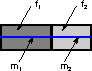
\includegraphics[width=0.9\linewidth]{../Common/images/Align_interaction_part.pdf}}  &  
\adjustbox{valign=t}{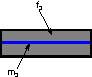
\includegraphics[width=0.9\linewidth]{../Common/images/Align_interaction_midsurf.pdf}} &  
Both $m_1$ and $m_2$ remain unchanged.
\\ \midrule

Overlap  &
\adjustbox{valign=t}{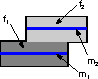
\includegraphics[width=0.9\linewidth]{../Common/images/Overlap_interaction_part.pdf}}  &  
\adjustbox{valign=t}{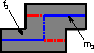
\includegraphics[width=0.9\linewidth]{../Common/images/Overlap_interaction_midsurf.pdf}} &  
 The extra patches are removed from both $m_1$ and $m_2$, whereas both are joined with an additional patch.
\\
\bottomrule
\end{longtable}
%}
\label{tbl:midsurfcelljoin:midsurfinteraction}
\end{center}
%\end{table}

%%\bigskip


Table \ref{tbl:midsurfcelljoin:midsurfinteraction} illustrates some of the representative configurations of interaction of two face pairs (or features), along with their corresponding midsurface patches. Face pairs (or features) $f_1$ and $f_2$ include $m_1$ and $m_2$ as their corresponding midsurface patches. Both interact in multiple ways, which can be commonly referred to as `L', `T', `X', Align and Overlap configurations. Each configuration needs different adjustments to midsurface patches to get them connected.


The first row of Table \ref{tbl:midsurfcelljoin:midsurfinteraction} shows the configuration type `L'. The first picture depicts interaction of face pairs f1 and f2 and the second picture shows adjustments needed to connect two midsurface patches $m_1$ and $m_2$ i.e. $m_2$ needs to be extended to meet $m_1$, whereas $m_1$ needs to be trimmed.

The second row of Table \ref{tbl:midsurfcelljoin:midsurfinteraction} shows the configuration type `T', where two midsurface patches get connected by logic: $m_2$ needs to be extended to meet $m_1$, whereas $m_1$ remains unchanged.

Similarly further rows elaborate remaining configuration types. The table clearly shows that developing the midsurface patch joining logic involves dealing with a variety of different configurations, which need to be addressed on case-by-case basis. This makes devising a generic midsurface patch joining approach, a challenging task. \deleted{real life models can have even more configurations than shown in Table \ref{tbl:midsurfcelljoin:midsurfinteraction}. Such unaccounted cases also manifests in the form of midsurface errors such as gaps, overlaps, etc.} Thus failures to join midsurface patches are very common and manifest in the form of gaps, overlaps, etc.


\todo{Review comment: Add figures for errors. [DONE]}

%%%\bigskip


 
%%\bigskip


 \begin{figure}[h!]
\centering     %%% not \center
\subfloat[Gaps]{\label{fig_midsurfgap}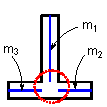
\includegraphics[width=0.23\linewidth]{../Common/images/midsurfgap.pdf}} \quad
\subfloat[Overlaps]{\label{fig_midsurfoverlap}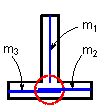
\includegraphics[width=0.23\linewidth]{../Common/images/midsurfoverlap.pdf}} \quad
\subfloat[Extra Extension]{\label{fig_midsurfextra}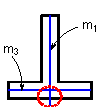
\includegraphics[width=0.23\linewidth]{../Common/images/midsurfextra.pdf}} 
\subfloat[Missing Patches]{\label{fig_midsurfmissing}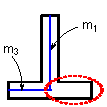
\includegraphics[width=0.23\linewidth]{../Common/images/midsurfmissing.pdf}} 
\caption{Typical Errors in Generating Connected Midsurfaces}
  \label{fig:midsurfcelljoin:midsurferrors}
\end{figure}
 
%%\bigskip

Figure~\ref{fig:midsurfcelljoin:midsurferrors} shows some of the commonly occurring midsurface errors. Figure~\ref{fig_midsurfgap} shows that midsurface patches ($m_1,m_2,m_3$) could not extend properly thus resulting in gaps between them. Figure~\ref{fig_midsurfoverlap} shows that two of the patches ($m_2,m_3$) got extended more than necessary thus resulting in overlaps. Figure~\ref{fig_midsurfextra} shows that one patch ($m_1$) got extended so much that the midsurface went out of the model's boundaries. Figure~\ref{fig_midsurfmissing}  shows that one of the patches ($m_2$, not shown) did not get created at all.


 To get the idea of gravity of this challenging problem,  Figure~\ref{fig_comm} shows the output of automatic midsurfacing by two of the leading CAD-CAE commercial systems, which primarily use face Pairing approach.
 
CAD models of English alphabets are chosen for benchmarking as they are easy to understand and represent a wide variety of shapes and interaction types found in the real-life thin-walled parts. Figures \ref{fig_mcad} and \ref{fig_mcae} demonstrate the midsurface failures such as missing surfaces, gaps, not lying midway, etc.
\todo{Review comment: These figures are not clear. [ENLARGED]}

\def \myfigcommcolumnwidth{0.55}

%
%%%\bigskip
% 
%\begin{figure}[htbp]
%\centering     %%% not \center
%\subfloat[CAD Models]{\label{fig_mmodel}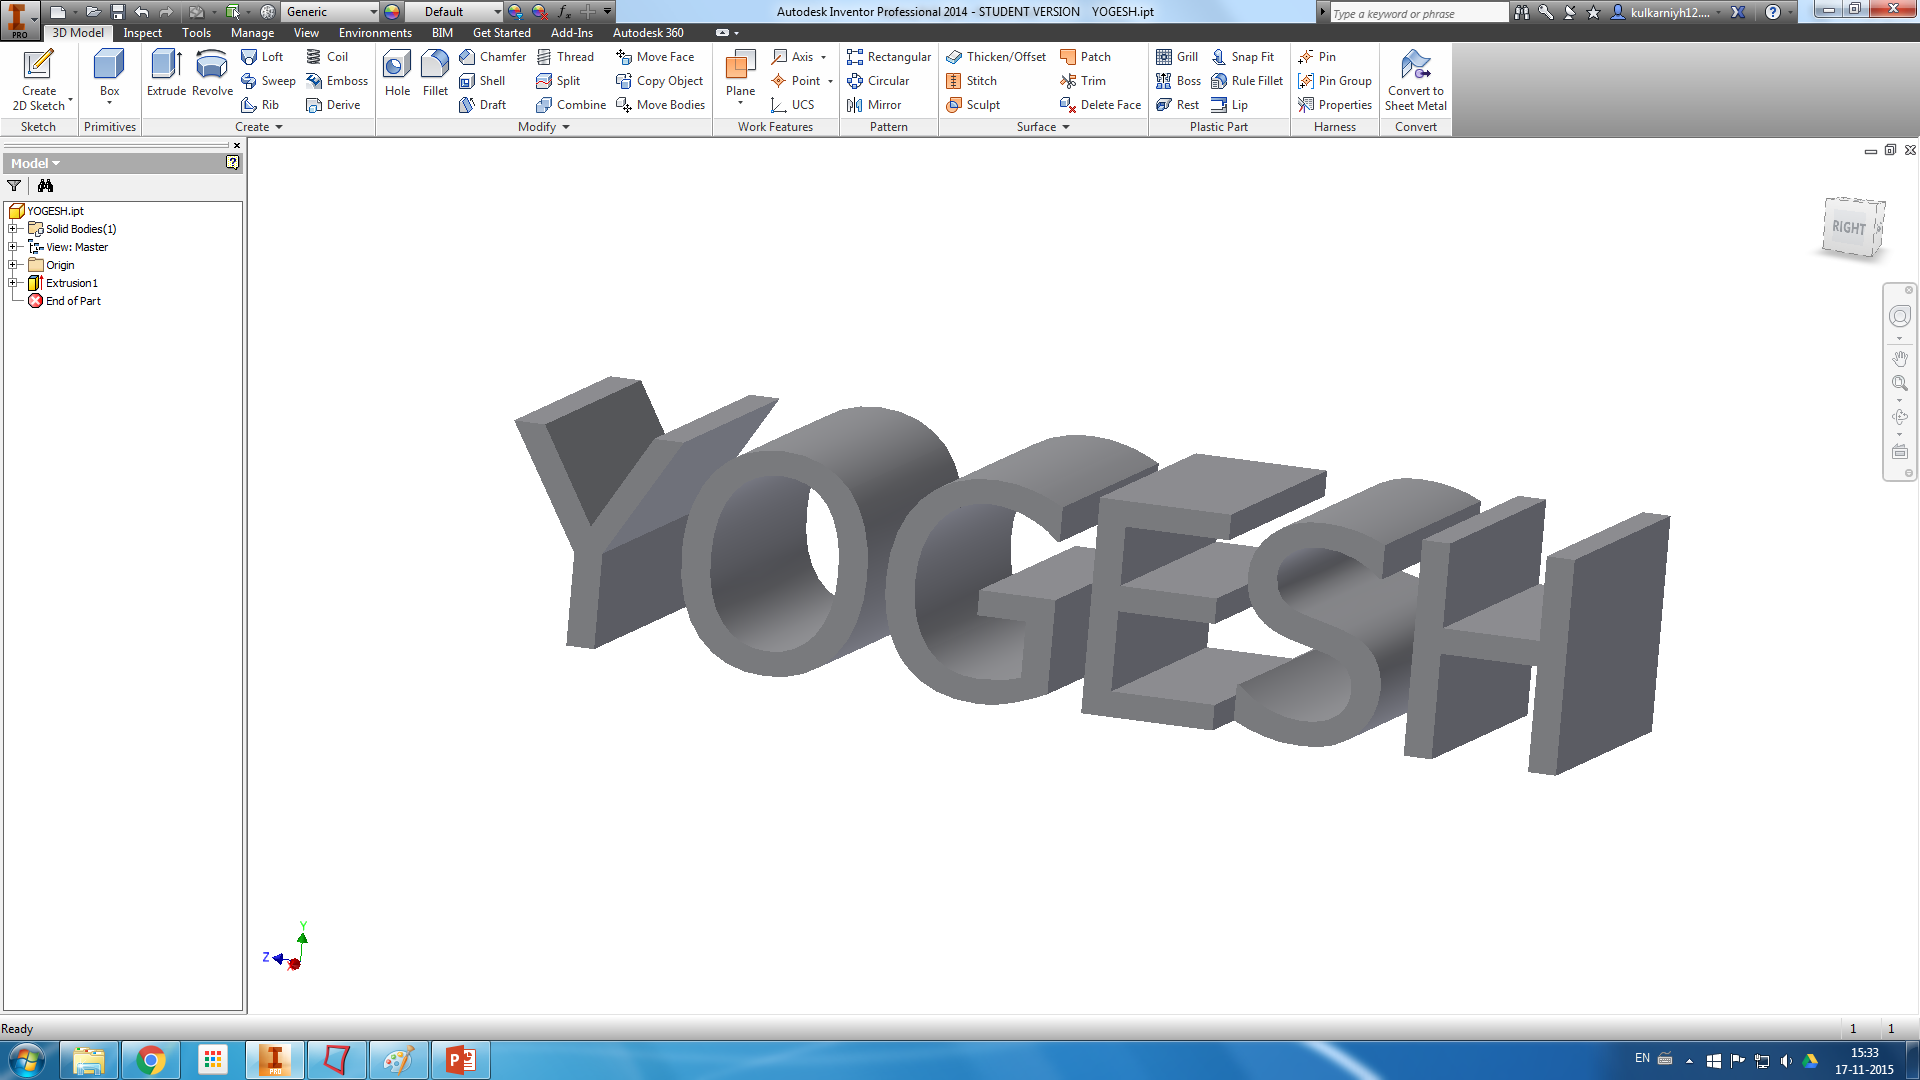
\includegraphics[width=\myfigcommcolumnwidth\linewidth]{../Common/images/Yogesh_Inv}} \quad
%\subfloat[Midsurface: Application 1]{\label{fig_mcad}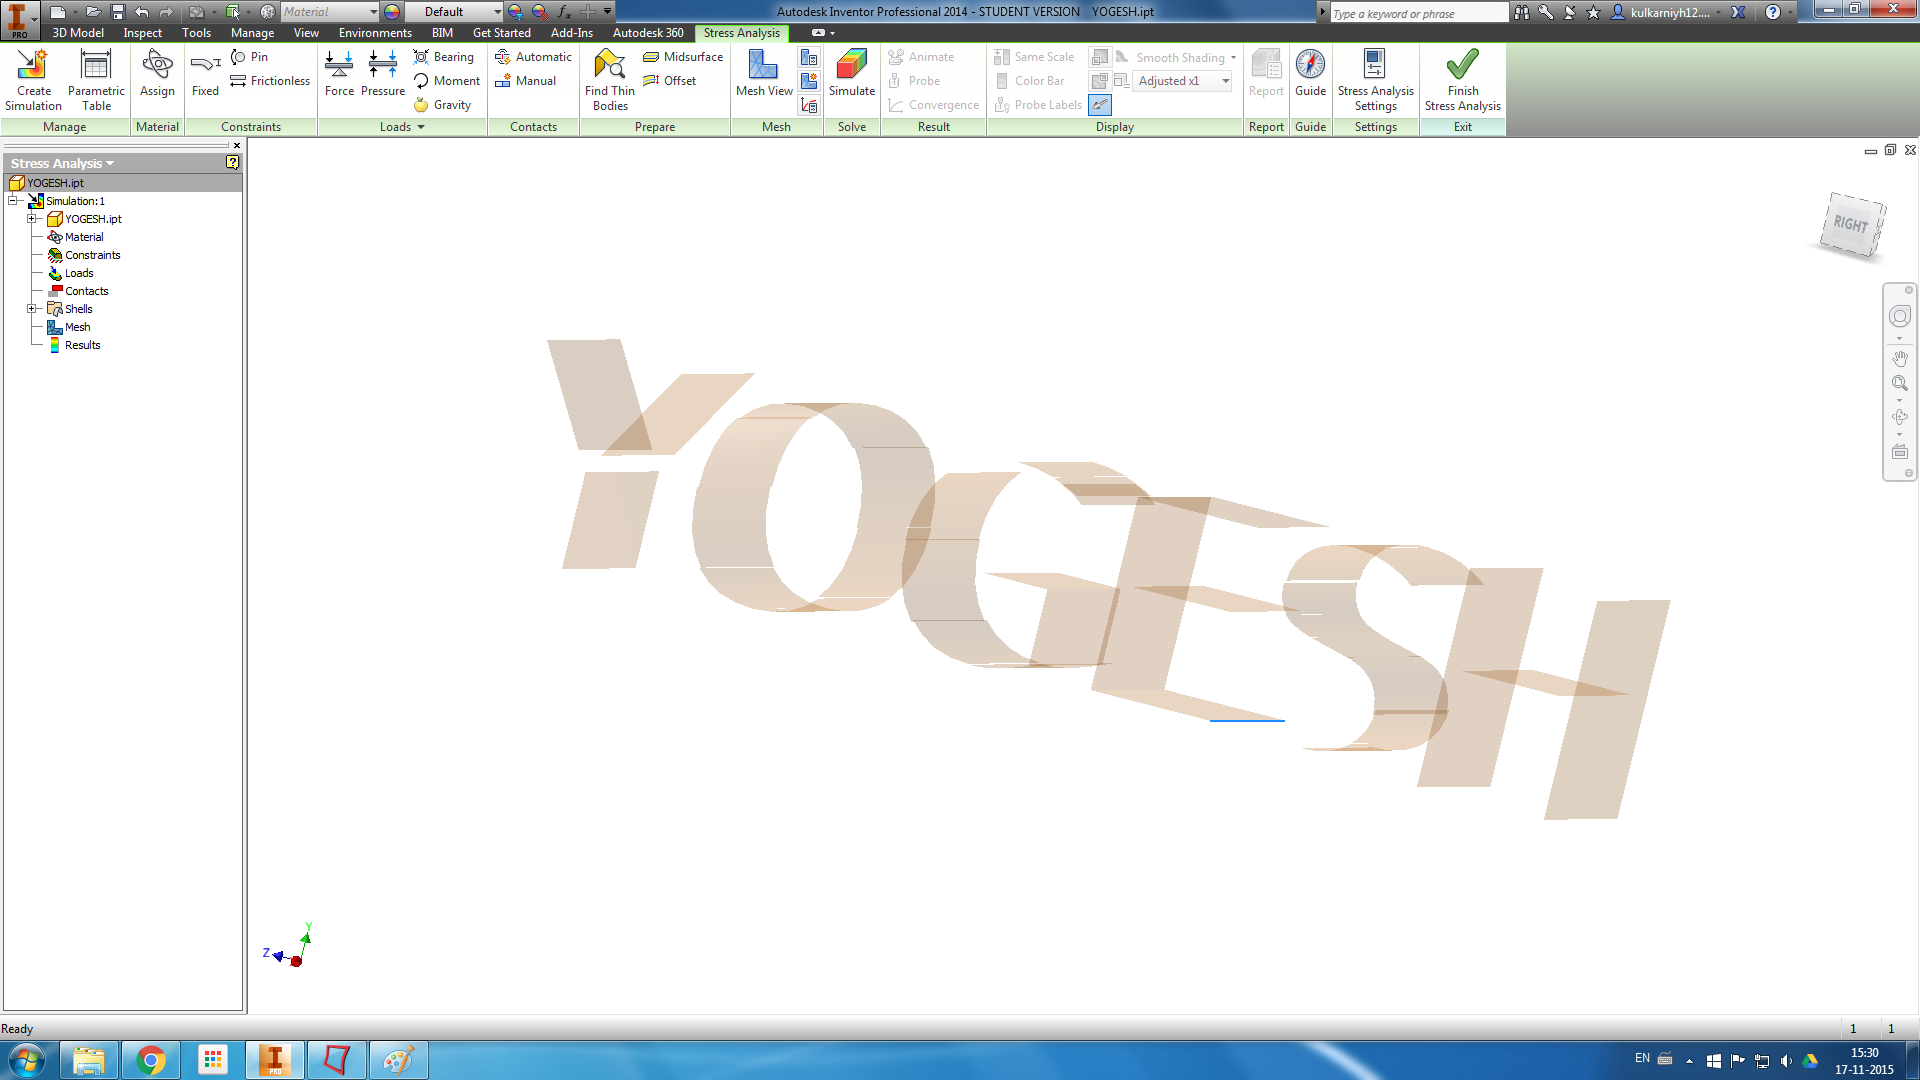
\includegraphics[width=\myfigcommcolumnwidth\linewidth]{../Common/images/Yogesh_InvMids}} \quad
%\subfloat[Midsurface: Application 2]{\label{fig_mcae}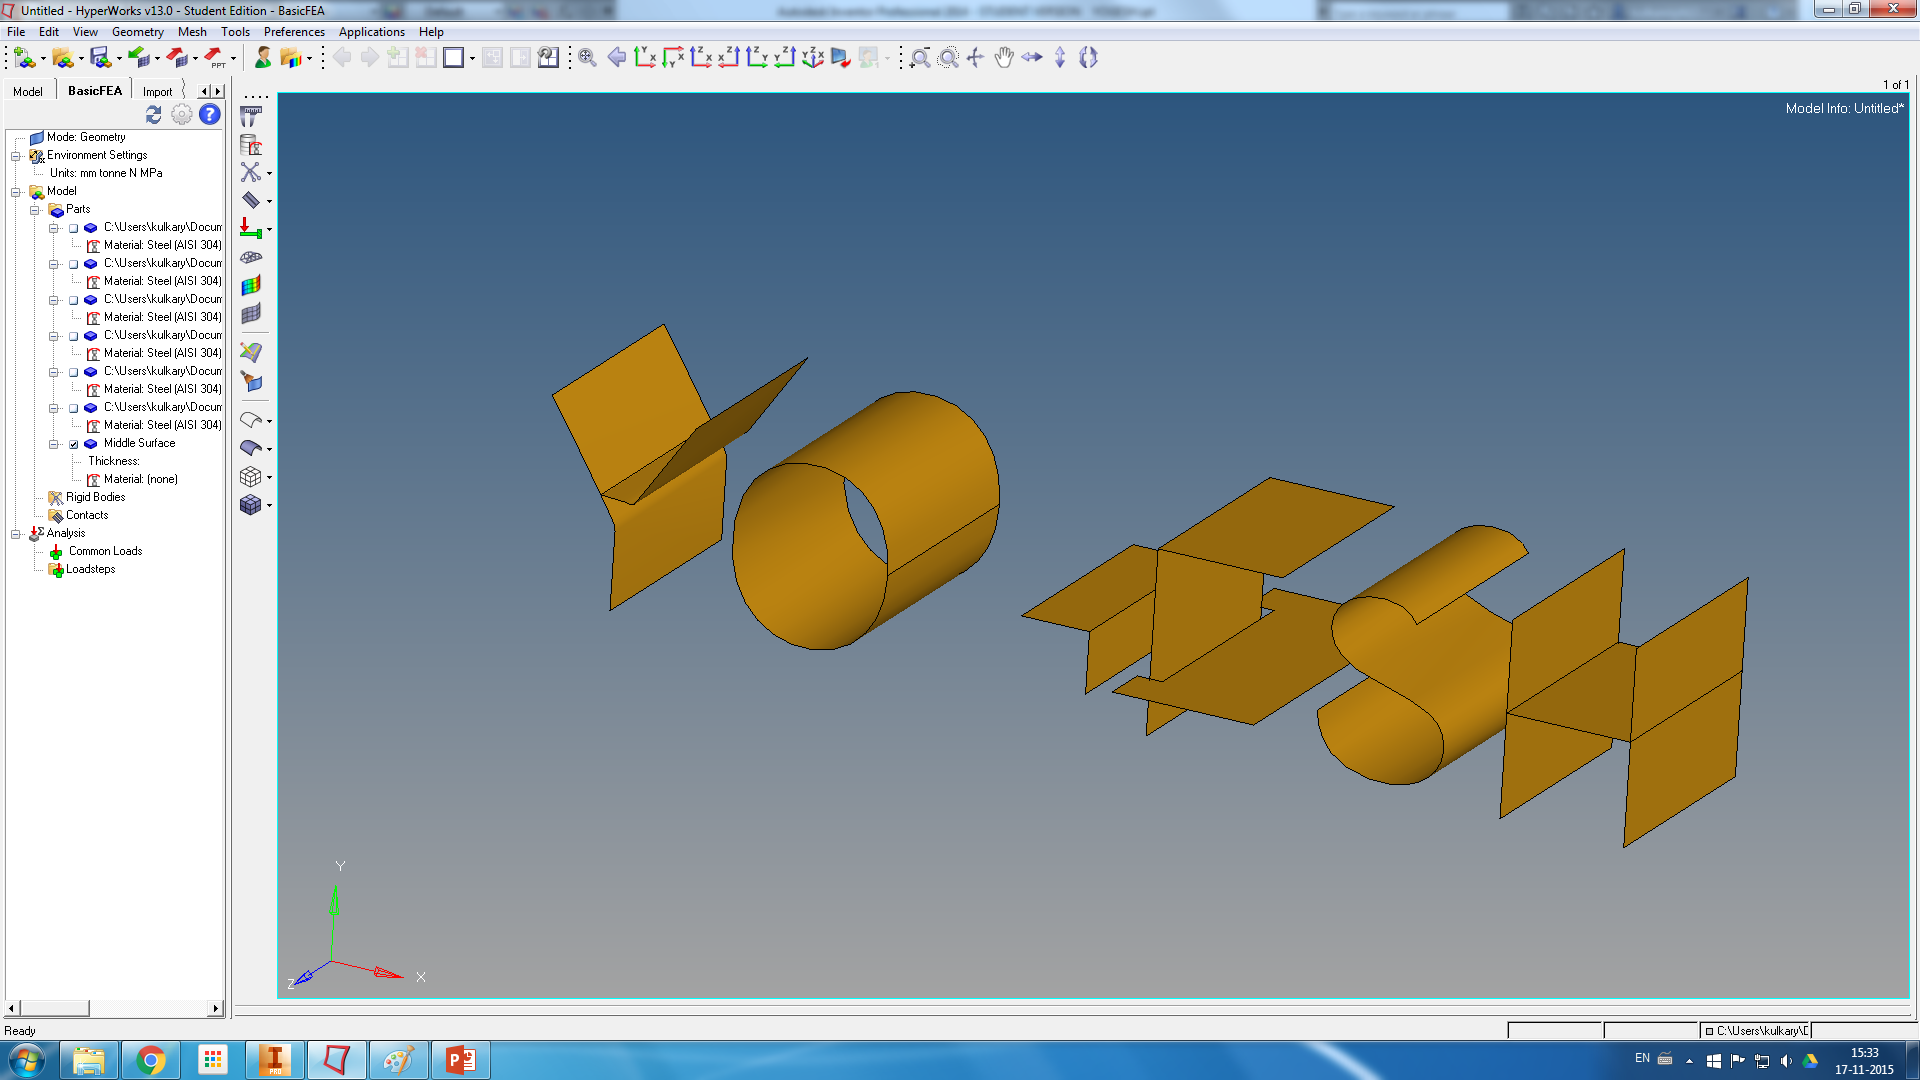
\includegraphics[width=\myfigcommcolumnwidth\linewidth]{../Common/images/Yogesh_HM_notOK}} 
%\caption{Midsurface outputs of commercial applications}
%  \label{fig_comm}
%\end{figure}
%
%
%%%\bigskip
% 
Developing a generic logic for joining midsurface patches is thus the need of the hour. As there is no theoretical framework encompassing all the possible interaction types, so far an unified logic has not been possible~\cite{Stolt2006}.  

The present research leverages generalized feature-based CAD model to address the issues related to face pairing. It proposes to use cellular decomposition approach to address the problems of midsurface patch joining. 

\subsection{Using Feature Information Instead of Face Pairing}
As seen in Section \ref{sec:midsurfcelljoin:facepairdetection} detecting face pairs is a challenging and error prone task. Information stored in the features in the feature-based CAD model has potential of replacing the need of face pairing altogether. In feature-based CAD modeling paradigm, model is built step-by-step using features. At each step, a new feature is booleaned to (i.e.`added to' or `subtracted from') the existing model, \replaced{thus making final model at the end}{at the end, making final, often complex shape}.

%%%\bigskip
%
%\begin{figure}[h!]
%	\centering 
%	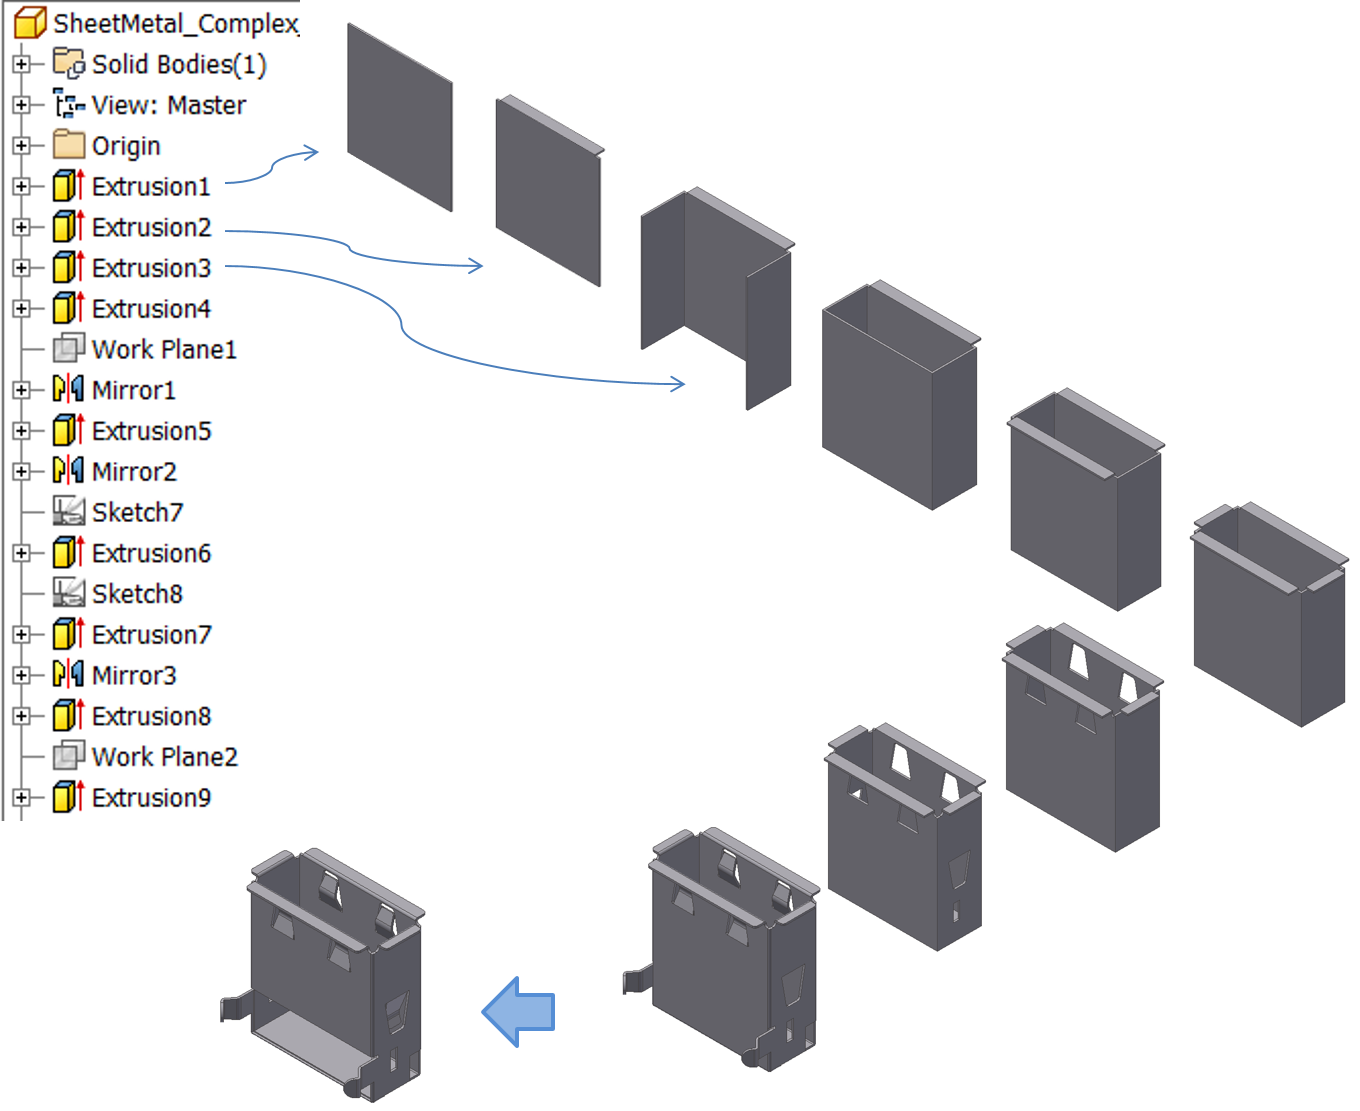
\includegraphics[width=0.75\linewidth]{../Common/images/usbfeaturetree}
%	\caption{Feature based construction of USB CAD model}
%	\label{fig:midsurfcelljoin:usbfeaturetree}
%	\end{figure}
%	
%
%%%\bigskip
%
%Figure \ref{fig:midsurfcelljoin:usbfeaturetree} shows a CAD model USB  built by booleaning features at each step. Looking at the final shape it is evident that detecting face-pairs in the final shape (B-rep) is complex task.
\deleted{Thus generating midsurface patches is challenging if worked on the B-rep. Instead, the} The present research proposes to use each feature's parameters to compute its own midsurface patch and thus avoiding the need of face pairing altogether. For example, Extrude feature computes its own midsurface using own sketch-profile and other parameters. This idea is advantageous, because, it not only avoids the problems of face pairing but it is also regenerates models upon parameter changes. \added{Whenever a feature undergoes any dimension change, only the dependent features are updated to maintain the validity and constraints defined in the model.}Thus, in the idea of computing midsurface from feature parameters, only the features which have updated need to re-compute the midsurface patches, whereas in the traditional face pairing approach, the whole model needs to be reevaluated for face pair detections and midsurface computations\deleted{upon any model updates}.

One of the limitations of using features in midsurface computation is the variety of features present in a typical sheet metal parts CAD model. All these features would need to have their own logic of computing midsurface patches. \deleted{, thus devising the midsurface computation logic is highly laborious task.} Another limitation is that even after implementation is over with the available set of features, introduction of any new feature would need additional logic for computing their own midsurface patches. These problems can be avoided by \replaced{proposing use of generalized features, i.e. $\mathcal{ABLE}$ model}{using generalized CAD model using $\mathcal{ABLE}$} paradigm. As elaborated in Chapter \ref{ch:Abstraction}, $\mathcal{ABLE}$ models are made up of only a set of loft-equivalent features such as Extrude, Revolve, Sweep and Loft. With $\mathcal{ABLE}$ model as input, the midsurface patch generation needs to be implemented only for limited number of  loft-equivalent features.

\todo{Review comment: Not yet true, so don't mention here}

\deleted{Thus the proposed approach addresses the original problem of face pairing by leveraging feature information and it addresses the problem of variety of features by using a reduced set of $\mathcal{ABLE}$  features, thereby} Thus the proposed solution of using $\mathcal{ABLE}$ model avoids face pairing altogether, making midsurface patch generation less error prone.

\subsection{Using Feature-based Cellular Topology for Joining Patches}

In Section~\ref{sec:midsurfcelljoin:facepairinteraction}, Table \ref{tbl:midsurfcelljoin:midsurfinteraction} showed a variety of configurations in which midsurface patch joining takes place in the existing face pairing approaches. \replaced{It can be clearly seen that there are a variety of configurations that need to be solved for connecting midsurface patches. The reported past  approaches have not demonstrated any generic approach to solve them generically, i.e. with a singular rule.}{These cases have their own patch joining logic, making algorithm development cumbersome and error-prone.}

The present research \replaced{uses}{proposes} feature-based cellular topology (FBCT) to address the problems in joining midsurface patches. Figure \ref{fig:midsurfcelljoin:featureinteractions} shows a schematic representation of a typical feature interaction, explains the context of feature-based cellular decomposition (FBCD), its outcome i.e. FBCT and its advantage in devising generic midsurface patch joining approach.

\todo{Review comment: I think you need to describe cellular decomposition of a generalized feature-based CAD model and then come to this point. [THIS SECTION IS ONLY DESCRIBE RESOLUTION OF MIDSURFACE PATCH JOININNG. FBCD IS DETAILED LATER]}

%%\bigskip

\begin{figure}[h!]
\centering     %%% not \center
\subfloat[Features]{\label{fig_twofeat}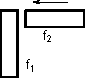
\includegraphics[width=0.21\linewidth]{../Common/images/twofeatures1.pdf}} \quad
\subfloat[Boolean]{\label{fig_featbool}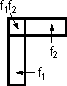
\includegraphics[width=0.17\linewidth]{../Common/images/featuresboolean1.pdf}} \quad
\subfloat[FBCD]{\label{fig_fbcdfig}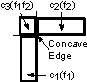
\includegraphics[width=0.23\linewidth]{../Common/images/fbcdfig1.pdf}} 
\subfloat[FBCT with Midsurface]{\label{fig_mpatch}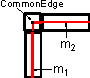
\includegraphics[width=0.235\linewidth]{../Common/images/patchinteraction1.pdf}} 
\caption{Feature Interactions and Cellular Decomposition}
  \label{fig:midsurfcelljoin:featureinteractions}
\end{figure}

%%\bigskip

Figure \ref{fig_twofeat} shows feature $f_2$ getting booleaned to the existing model, denoted by feature $f_1$. After boolean, both features are merged with some portion (shown as $f_1f_2$) of $f_2$ getting consumed inside $f_1$, as seen in Figure \ref{fig_featbool}. Figure \ref{fig_fbcdfig} depicts the cellular decomposition with cells having owner features such as $c_1(f_1)$, $c_2(f_2)$ and $c_3(f_1f_2)$. Figure~\ref{fig_mpatch} shows same cells with midsurface patches computed for each. Table \ref{tbl:midsurfcelljoin:midsurfinteraction} clearly indicates that $f_1f_2$ portion is the place where midsurface patches interact differently in different configurations. 

Cellular decomposition refers to technique of decomposition of a shape into sub-shapes called cells. 
\todo{Review comment: Do not need this para here. Add high level need. [DONE]}
Primary advantage of cellular decomposition is simplification. Instead of working on complex shapes, cells having primitive shapes, are easier to handle. For example, instead of meshing whole model, cells are meshed based on their characteristics. Cellular decomposition not only reduces the number of types of shapes to be handled, but also creates a possibility of working on them parallelly. Because of such substantial advantages, cellular decomposition has been used in variety of domains such as CAM for pocket machining, CAE for isolating sub-volumes with different meshing patterns, CAD model transitions with different level of details (LoDs), etc. Cellular Decomposition suffers from certain limitations as well. The choice of locations and cutting-geometries for decomposition decides the quality of resultant decomposition. Wrong choices result in a large number of redundant cells or in the cells which are not of primitive shapes. 


\section{Proposed Approach for Midsurface Computation}  \label{sec:midsurfcelljoin:proposal}
As discussed in the previous sections, two of the most critical problems faced in the face pairing approach are, face pair detection and midsurface patch joining.  The present research proposes to leverage generalized Loft-equivalent features to address the issues related to face pairing and use feature-based cellular topology to address the problems of midsurface patch joining. \deleted{Following subsections detail the rational of these proposals and their advantages.} The proposed solution is to separate out the common area by decomposition, so that generic rules for joining midsurface patches, can be derived. 

%%Figure \ref{fig_fbcdfig} shows feature based cellular decomposition (FBCD) of the input model into 3 ``cells''. This decomposition happens at the concave edge shown as dot in Figure \ref{fig_fbcdfig}. The cutting-geometry lines (cutting planes in 3D) are shown with dotted lines. The resultant cells do not have any volumetric overlapping, they touch each other only at the boundaries. Cells retain their owner feature information. Thus, cell $c_1$ has owner feature $f_1$, $c_2$ has owner feature $f_2$ and the common portions cell $c_3$ has two owners $f_1,f_2$.
%%
%%%Using both, $\mathcal{ABLE}$ and FBCT, following section presents the proposed algorithm to compute a quality midsurface of sheet metal feature-based CAD model.
%%%
%%%Chapter~\ref{ch:Abstraction} has already elaborated the approach of transforming sheet metal feature based CAD model to generalized CAD model called $\mathcal{ABLE}$. Following section explains the cellular decomposition along with its state of the art. \deleted{Following sections presents the proposed approach that leverages cellular decomposition to devise a generic, singular logic for midsurface patch joining algorithm.}
%%
%%In the proposed approach, the midsurface patch joining rule is that cells $c_1$ and $c_2$ are delegated to compute midsurface patches $m_1, m_2$, whereas common cell $c_3$ (the one with two owners $f_1, f_2$) is delegated to join the incident midsurface patches $m_1, m_2$. This rule is singular and generic, applicable not only to all the cases in mentioned Table \ref{tbl:midsurfcelljoin:midsurfinteraction} but also to the cases found in real life part models. %Thus feature based cellular decomposition allowed formulation of singular, generic midsurface patch joining logic.
%%%\subsection{Proposed Algorithm for Computing Midsurface}  \label{sec:midsurfcelljoin:algorithm}
%%%The proposed midsurface computation approach is presented in the following sections. 

The generalized feature-based CAD model is suitably decomposed into manageable cell volumes. Cells are classified into solid cells ($sCell$) and interface cells ($iCell$). Midsurface patches are first computed from $sCell$s and are then joined in the $iCell$s.  The detailed treatment is presented in the sections to follow. To begin with Cellular Decomposition approaches are reviewed in the below section.

%Algorithm \ref{alg_FBDMidsurf} shows the pseudo-code view of the overall approach presented in Chapter \ref{ch:Proposal}. It can be seen that, the input sheet metal feature based CAD model has been simplified by defeaturing, before this module for computing midsurface (Algorithm \ref{alg_FBDMidsurf}, line: 1). Remaining features have got transformed to generalized Loft-equivalents ( Algorithm \ref{alg_FBDMidsurf}, line: 2). 
%
%%%\bigskip
%
%
%\begin{algorithm}[!h]
%\caption{Feature-based midsurface computation}
%\label{alg_FBDMidsurf}
%\begin{algorithmic}[1]
%	\REQUIRE Sheet metal Feature-based CAD model ($smfbcd$)
%	\STATE $defeatured\_model = feature\_based\_defeaturing(smfbcd)$
%	\STATE $generalized\_model = feature\_based\_generalization(defeatured\_model)$
%	\STATE $decomposed\_model =feature\_based\_cellular\_decomposition(generalized\_model)$
%	\STATE $G(n,e ) = populate\_graph(decomposed\_model)$
%	\STATE $(sCell,iCell) = classify\_cells((Gn,e))$
%	\FORALL{$sCell$}
%		\STATE $compute\_midsurface\_patch(sCell)$ (Algorithm \ref{alg:midsurfcelljoin:MidsurfsCell})
%	\ENDFOR
%	\FORALL{$iCell$}
%		\STATE $join\_midsurface\_patches(iCell)$ (Algorithm \ref{alg:midsurfcelljoin:MidsurfiCell})
%	\ENDFOR
%\end{algorithmic}
%\end{algorithm}
%
%%%\bigskip
%
%%Following sections elaborate the further steps (Algorithm \ref{alg_FBDMidsurf}, line: 3 onwards). 
%
%The generalized model, i.e. the $\mathcal{ABLE}$ model, is then decomposed by feature based cellular decomposition to form cells (Algorithm \ref{alg_FBDMidsurf} line:3) while retaining their respective $\mathcal{ABLE}$ owner features. The cells are then classified as solid cells ($sCell$) and interface cells ($iCell$) and are delegated with the task of computing the midsurface patches and joining them, respectively (Algorithm \ref{alg_FBDMidsurf} lines: 5 onwards ). 
%In proposed algorithm, both the problems of traditional face-pairing approach, i.e. face pair detection and multiple cases of patch joining, have been avoided completely. Thus the proposed algorithm reduces the midsurface errors present in the traditional approach of face pairing.
%
%Following section elaborates on how lacunae in face pairing approach have been avoided by leveraging Cellular Decomposition (CellDecomp) and feature-based cellular topology (FBCT).
%Both, CellDecomp and FBCT, have been part of the CAD domain for years, but their usage together, as a hybrid concept, is uncommon and has been proposed in the present work. Following sections elaborate more on this hybrid approach and its usage in the computation of the midsurface (Algorithm \ref{alg_FBDMidsurf} lines 3-11). 
%
%Following section elaborates on how Feature-based cellular topology is arrived at by decomposing $\mathcal{ABLE}$ feature based CAD model.



%\section{Feature-based Cellular decomposition of CAD Model} 
%\label{sec:midsurfcelljoin:decomposition}


\subsection{Literature Review of Cellular Decomposition}

Cellular decomposing has been researched extensively, especially for CAM applications~\cite{Ma2009}. Manufacturing sequences need different cells to be assigned with different machining processes. Generation of such cells is done by cellular decomposition of the CAD model such as Brep model. Similarly, in CAE, identification and separation of cells is carried out to assign different meshing patterns to different cells. Following are some of the relevant past approaches for cellular decomposition:

Bih-Yaw Shih \cite{Shih1996} presented an automated swept volume detection and decomposition algorithm for \added{hexahedral mesh generation}. This approach was computationally intensive for complex model. 

Yong Lu \cite{LuGadhTautges2001} reported the work on shape recognition and volume decomposition to automatically decompose a CAD model into hex meshable volumes. 

Yoonhwan Woo \cite{Woo2002} \cite{Woo2003} \cite{Woo2003a} \cite{Woo2006} \cite{Woo2009}  did extensive work in fast and maximal cellular decomposition. He found that in typical cell decomposition, each of the faces having a concave edge, act as cutting geometries and are extended spanning whole model, generating a large number of cells. Many of them were redundant. To avoid this he proposed a concept of `maximal volume'. 

Figure \ref{fig:litsurvey:maxcd} depicts Woo's process in which (a) shows the input model and (b) shows result of the cellular decomposition, generating large number of cells. His process combines cells based on certain criteria. Figure \ref{fig:litsurvey:maxcd}c shows the output having far lesser number of cells, i.e. just 2 cells having primitive shapes. 
 
 %%\bigskip
 
\begin{figure}[!h]
\centering     %%% not \center
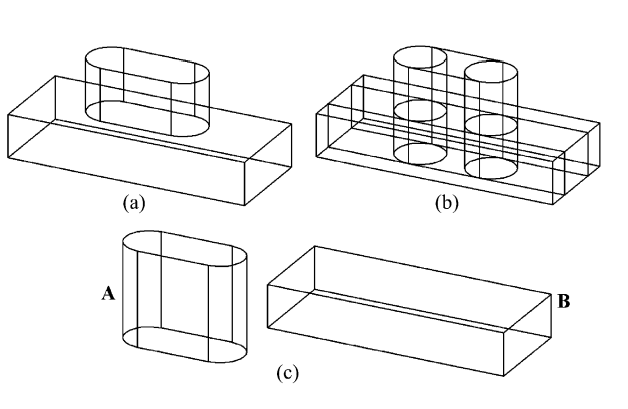
\includegraphics[width=0.7\linewidth,valign=t]{../Common/images/WooMax}
\caption{Maximal Cellular Decomposition (Source : Woo \cite{Woo2003})}
\label{fig:litsurvey:maxcd}
\end{figure}

%%\bigskip

Woo's method was superior to other prevalent methods but was restricted to shapes with analytical surfaces only.
 

%%Review of the cellular decomposition approaches suggests that, \deleted{although it is widely used in CAM, it has found limited usage in CAD modeling applications. T}the cost of creating cells and maintaining their connectivity and validity during the CAD modeling operations far outweighs the flexibility they provide. That is the reason, cellular decomposition has not been hugely popular in CAD systems. 

%Following subsection reviews reported approaches of feature based cellular topology, generated when cellular decomposition is performed on feature based CAD model.
 
%\subsection{Literature Review of Feature-based Cellular Topology}
 
 \todo{Review comment: Whats the connection between these  Lit survey paragraphs. [IT HAS BEEN EXPLAINED JUST BEFORE THESE SURVEYS]}
 
The result of Cellular Decomposition is a collection of cells, termed as `cellular topology (CT)' model~\cite{Chen2006}. \todo{Review comment: Here state what are the downstream applications that use decomposed cad model. [DONE]}
Cellular decomposition of a feature-based CAD model results in feature-based cellular topology (FBCT) model. Figure \ref{fig:litsurvey:fbct} shows one such example of FBCT model, in which, $cell 1$ has $block$ as the owner feature whereas $cell 2$ is the common cell for features $block$ and $roundedRectPocket$, etc. %So, all the overlapping feature portions have been decomposed into cells with those features as owners. In Feature-based cellular topology, thus, there are not overlapping solid cells. They touch each other, fully at cells boundary surfaces.

%%\bigskip
 
 \begin{figure}[!h]
\centering     %%% not \center
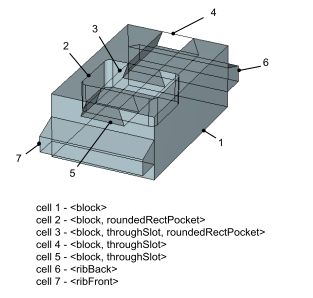
\includegraphics[width=0.62\linewidth,valign=t]{../Common/images/fbct}
\caption{Feature-based Cellular Topology (Source : Bidarra \cite{Bidarra2003a})}
\label{fig:litsurvey:fbct}
\end{figure}

%%\bigskip

%The proposed research leverages CellDecomp of a feature based CAD model and generates FBCT.
\deleted{In one of the widely used CellDecomp method, called Concave Edge Partitioning (CEP), CAD model is partitioned at the concave edges with the partitioning tool as the extended faces incident at the concave edge. In Figure \ref{fig_fbcdfig} the concave edge is shown as big dot, whereas the dotted lines represent the partitioning tools. This method is also known Convex Partitioning as the resultant model contains only the convex cells.}

Cellular Topology (CT) is the solid modeling data structure having cells as the fundamental building block. Cells do not overlap volumetrically but touch each other only at surface boundaries. In Feature-based cellular topology (FBCT) cells have owner features. FBCT model has not yet been used widely, especially in commercial systems. Some of the relevant works in academic research are reviewed below. \deleted{In FBCT environment, feature operations such as creation, editing, deleting, are formulated in terms of cells with appropriate feature owners.}
\todo{Review comment: Give example of CT modeling operations. [DELETED THE LINE ITSELF. MAY NOT NEED TO ADD THESE DETAILS]}

Bidarra~\cite{Bidarra1993, Bidarra1997, BidarraKrakerBronsvoort1998} proposed feature based cellular topology to improve over the shortcomings of B-prep, such as complex boundary evaluation after any modeling operation. He built a FBCT system called $SPIFF$ in which features were assigned to cells of ACIS CT model. The system provided flexibility to choose specific cells for evaluating boundary for specific applications.

 %%\bigskip
 
\begin{figure}[!h]
\centering     %%% not \center
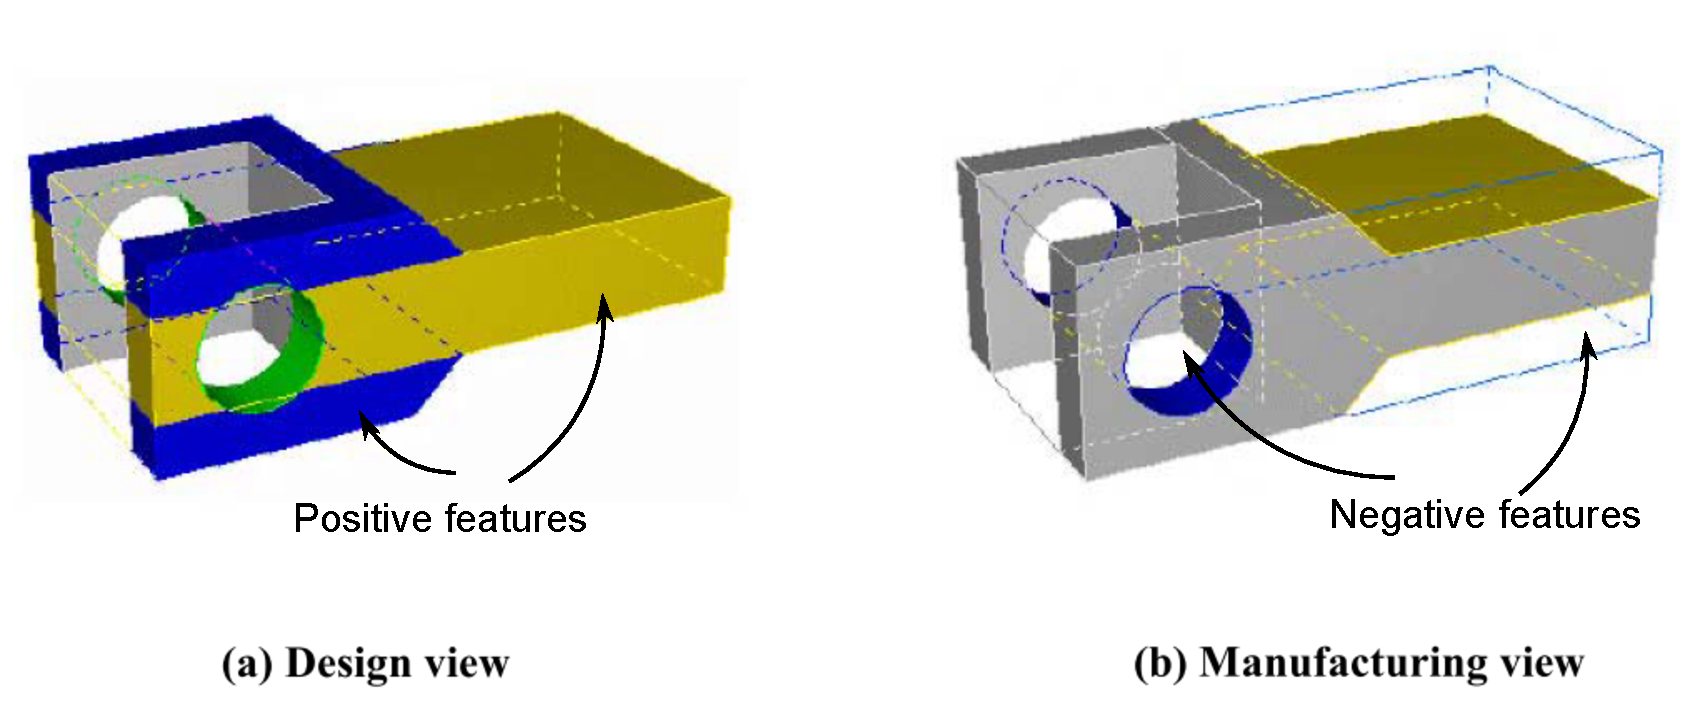
\includegraphics[width=0.85\linewidth,valign=t]{../Common/images/multiview.pdf}
\caption{Application Perspective Based Viewing of a Model (Source: Van~\cite{Van2000})}
\label{fig:litsurvey:multiview}
\end{figure}

%%\bigskip

Kraker \cite{Kraker1998} presented feature operations in cellular model for multi-view architecture. This architecture was used to selectively present cells as per need of client application. \added{For example, a design can see both additive and subtractive features, whereas manufacturing view of the same model can see only subtractive features. Figure~\ref{fig:litsurvey:multiview} shows these two views with an example. Use of positive and negative features is different in both the views, even though the model is same.}



%Although FBCT provided flexibility in modeling, the model would progressively become complex as number of features increased.

%Treek \cite{Treeck}, in altogether different domain of arcitecture, used cellular model for CAE analysis. He
%Quite a few attempts to compute the midsurface using cellular decomposition are found in the literature \cite{Chong2004, Cao2009,Cao2011,Woo2013}.
%
% Below is the summary of the relevant Cellular Decomposition approaches:
% 
%\csvreader[longtable=|p{0.17\linewidth}|p{0.11\linewidth}|p{0.2\linewidth}|p{0.2\linewidth}|p{0.17\linewidth}|p{0.17\linewidth}|,
%    table head=\toprule \bfseries Author & \bfseries Input& \bfseries  Method & \bfseries  Approach& \bfseries  Advantages& \bfseries  Limitations \\ \midrule \endhead,% \bottomrule \endfoot,
%  late after last line=\\\bottomrule,
%  before reading={\catcode`\#=12},after reading={\catcode`\#=6},    
%    late after line=\\\hline]%
%{../DocsSources/litsurvey_celldecomp.csv}{Author=\Author, Input=\Input, Method=\Method, Approach=\Approach, Advantages=\Advantages ,Limitations=\Limitations}%
%{\Author  & \Input&  \Method &\Approach & \Advantages & \Limitations}%
%
%Cellular decomposition, in the context of the current research, is the division of a feature based CAD model into non-volumetrically overlapping, but surface-overlapping sub-solids (called ``cells'').  
% 
%\csvreader[longtable=|p{0.17\linewidth}|p{0.11\linewidth}|p{0.2\linewidth}|p{0.2\linewidth}|p{0.17\linewidth}|p{0.17\linewidth}|,
%    table head=\toprule \bfseries Author & \bfseries Input& \bfseries  Method & \bfseries  Approach& \bfseries  Advantages& \bfseries  Limitations \\ \midrule \endhead,% \bottomrule \endfoot,
%  late after last line=\\\bottomrule,
%  before reading={\catcode`\#=12},after reading={\catcode`\#=6},    
%    late after line=\\\hline]%
%{../DocsSources/litsurvey_featurecells.csv}{Author=\Author, Input=\Input, Method=\Method, Approach=\Approach, Advantages=\Advantages ,Limitations=\Limitations}%
%{\Author  & \Input&  \Method &\Approach & \Advantages & \Limitations}%

\deleted{As the feature-based algorithms are not yet very prevalent, the feature based cellular topology data structures has shown limited usage in the practical CAD applications so far.}
\todo{Review comment: Summarize and comment. [ADDED BELOW]}
\added{Review of the past approaches show their wide applicability for the processes like machining, meshing, etc.  There are a large number of approaches developed to cater to various domains. The present research suitably leverages one of the feature-based cellular decomposition approach, a combination of Woo~\cite{Woo2002, Woo2003, Woo2003a, Woo2006, Woo2009} and Bidarra~\cite{Bidarra1993, Bidarra1997, BidarraKrakerBronsvoort1998} approaches. As the readily usable implementation of such combination is not available, a manual cellular decomposition approach was taken up, based on the methodology suggested in the said approaches.}
%% Assigning appropriate owner features and maintaining validity during feature operations becomes increasingly challenging with increase in the complexity of the model. All these aspects have resulted in limited usage of FBCT in feature based CAD approaches.}
Following section elaborates the approach taken in the present research.

\subsection{Proposed Feature-based Cellular Decomposition Approach}\label{sec:fbcd:proposal}

The primary objective of this module is to present an approach taken for decomposing a generalized feature based CAD model. Following steps elaborate the approach:
%The present research proposes using  FBCT created by feature-based Cellular Decomposition (FBCD) of $\mathcal{ABEL}$ feature based CAD model. 
%Primary steps used in FBCD are:
\begin{itemize}[noitemsep,topsep=2pt,parsep=2pt,partopsep=2pt]
\item \textbf{Feature separation}: A feature-based CAD model is built by Boolean of new features with the existing. Booleans are of ``Unite'', ``Subtract'', ``Intersect'' and ``New Body' types. \deleted{As the input model is defeatured before, the input model now primarily has only ``Unite'' type of booleans between features.} In this step, the ``Unite'' boolean type set between two features is removed and instead ``New Body'' type applied, thereby separating the tool bodies of the features.

%%\bigskip


  \begin{figure}[!h]
\centering     %%% not \center
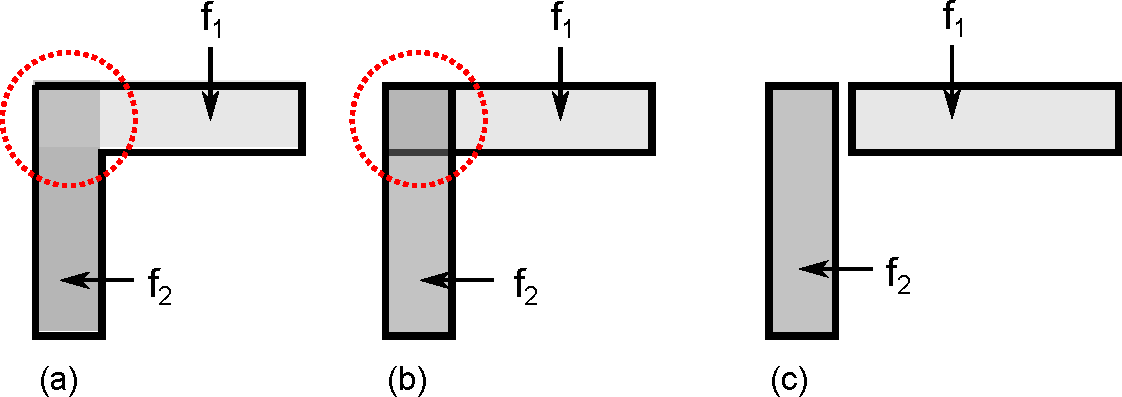
\includegraphics[width=0.75\linewidth,valign=t]{../Common/images/newbody_bw.pdf}
\caption{Separation of Feature Tool Bodies}
\label{fig:litsurvey:newbody}
\end{figure}

%%\bigskip


Figure~\ref{fig:litsurvey:newbody}a shows a model with two features $f_1$ and $f_2$ with ``Union'' type of boolean between them. Once the boolean type is changed, the tool-bodies of features get isolated, even though they are placed at the same location. Figure~\ref{fig:litsurvey:newbody}b shows that there is no connection left between them anymore.  Although Figure \ref{fig:litsurvey:newbody}c  depicts feature tool bodies in exploded view.% In reality, the features are at the same place as they were in Figure~\ref{fig:litsurvey:newbody}a.

 Thus, at this stage, all feature tool bodies are separated, however, spatially they may still overlap each other.
\todo{Review comment: Say adding in place of boolean. [NOT DONE AS BOOLEAN DOES NOT MEAN ADDING]}
\item \textbf{Concave edge partitioning (CEP)}:  Even after separating the feature tool bodies, there could be volumetric overlaps as seen in Figure~\ref{fig:litsurvey:newbody}b. In such cases, at this step, overlapping feature volumes are split at the concave edges, by a technique known as Concave edge partitioning (CEP) or Convex Partitioning (CP). It is a well established technique~\cite{Woo2002, Woo2003, Woo2003a, Woo2006, Woo2009}, where faces incident at a concave edge, are extended and used as cutting geometries to split the model.

%  \begin{figure}[!h]
%\centering     %%% not \center
%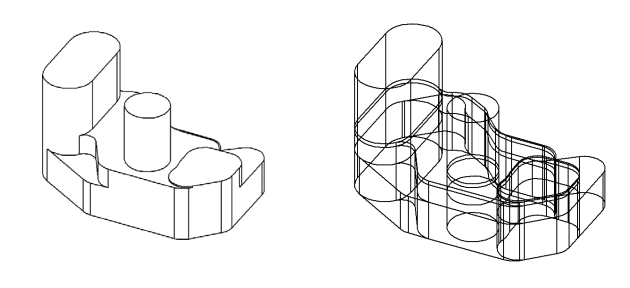
\includegraphics[width=0.75\linewidth,valign=t]{../Common/images/cep}
%\caption{Traditional Concave Edge Partitioning (Source : Woo \cite{Woo2003a})}
%\label{fig:litsurvey:cep}
%\end{figure}

\todo{Review comment: Use simple figures to explain. [DONE]}

%%\bigskip


  \begin{figure}[!h]
\centering     %%% not \center
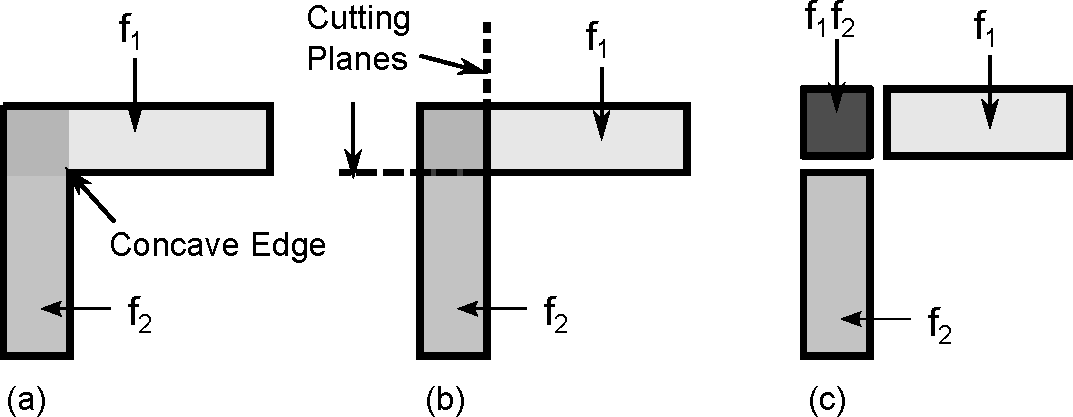
\includegraphics[width=0.75\linewidth,valign=t]{../Common/images/newcep_bw.pdf}
\caption{Concave Edge Partitioning}
\label{fig:litsurvey:newcep}
\end{figure}

%%\bigskip


Figure \ref{fig:litsurvey:newcep}a shows the the original input model. Decomposition is done at the concave edge by extending faces incident at it, as cutting geometries. Figure \ref{fig:litsurvey:newcep}b shows the cutting geometries (cutting planes in 3D). If the ``Union'' has been changed to `'New Body'' already, as mentioned in the previous step, large extensions need not be done. The existing faces of the separated tool bodies themselves act as cutting geometries.  Figure \ref{fig:litsurvey:newcep}c  shows decomposed cells in an exploded view. In the proposed work, the face extensions are not done infinitely (or going beyond the model's bounding box) but are restricted within the influence zone decided by the two interacting features. This enhancement avoids generation of a large number of redundant cells.
\end{itemize}

In some cases, the ``L'' shaped model as seen in Figure \ref{fig:litsurvey:newcep}a, may get created, not by booleaning two features $f_1$ and $f_2$ but as a single feature, say $f_3$, with ``L'' shaped profile. In such cases, CEP is not applied to the concave edge in $f_3$. As shown in the next stages, $f_3$ computes its own midsurface patch by computing midcurve of the profile and then extruding it.% This reduces computationally intensive cellular decomposition operations.

\todo{Review comment: So far you have not claimed that FBCD is your approach. [FBCD IS NOT FULLY MINE. SO SPECIFIED THAT CEP IS LEVERAGED BUT REST IS MINE]}

Out of the overall FBCD approach, the actual decomposition step (convex partitioning or CEP) has been leveraged from existing approaches, whereas the rest,i.e. feature assignment, localized partitioning, etc. are contributions of the present research work. Figure \ref{fig:midsurfcelljoin:beforecd} shows an example of CAD model of a sheet metal bracket and Figure \ref{fig:midsurfcelljoin:cd} is the output of FBCD, with each cell-bodies shown in different colors. 

%%\bigskip


\begin{figure}[!h]
\centering     %%% not \center
\subfloat[Input Model]{\label{fig:midsurfcelljoin:beforecd}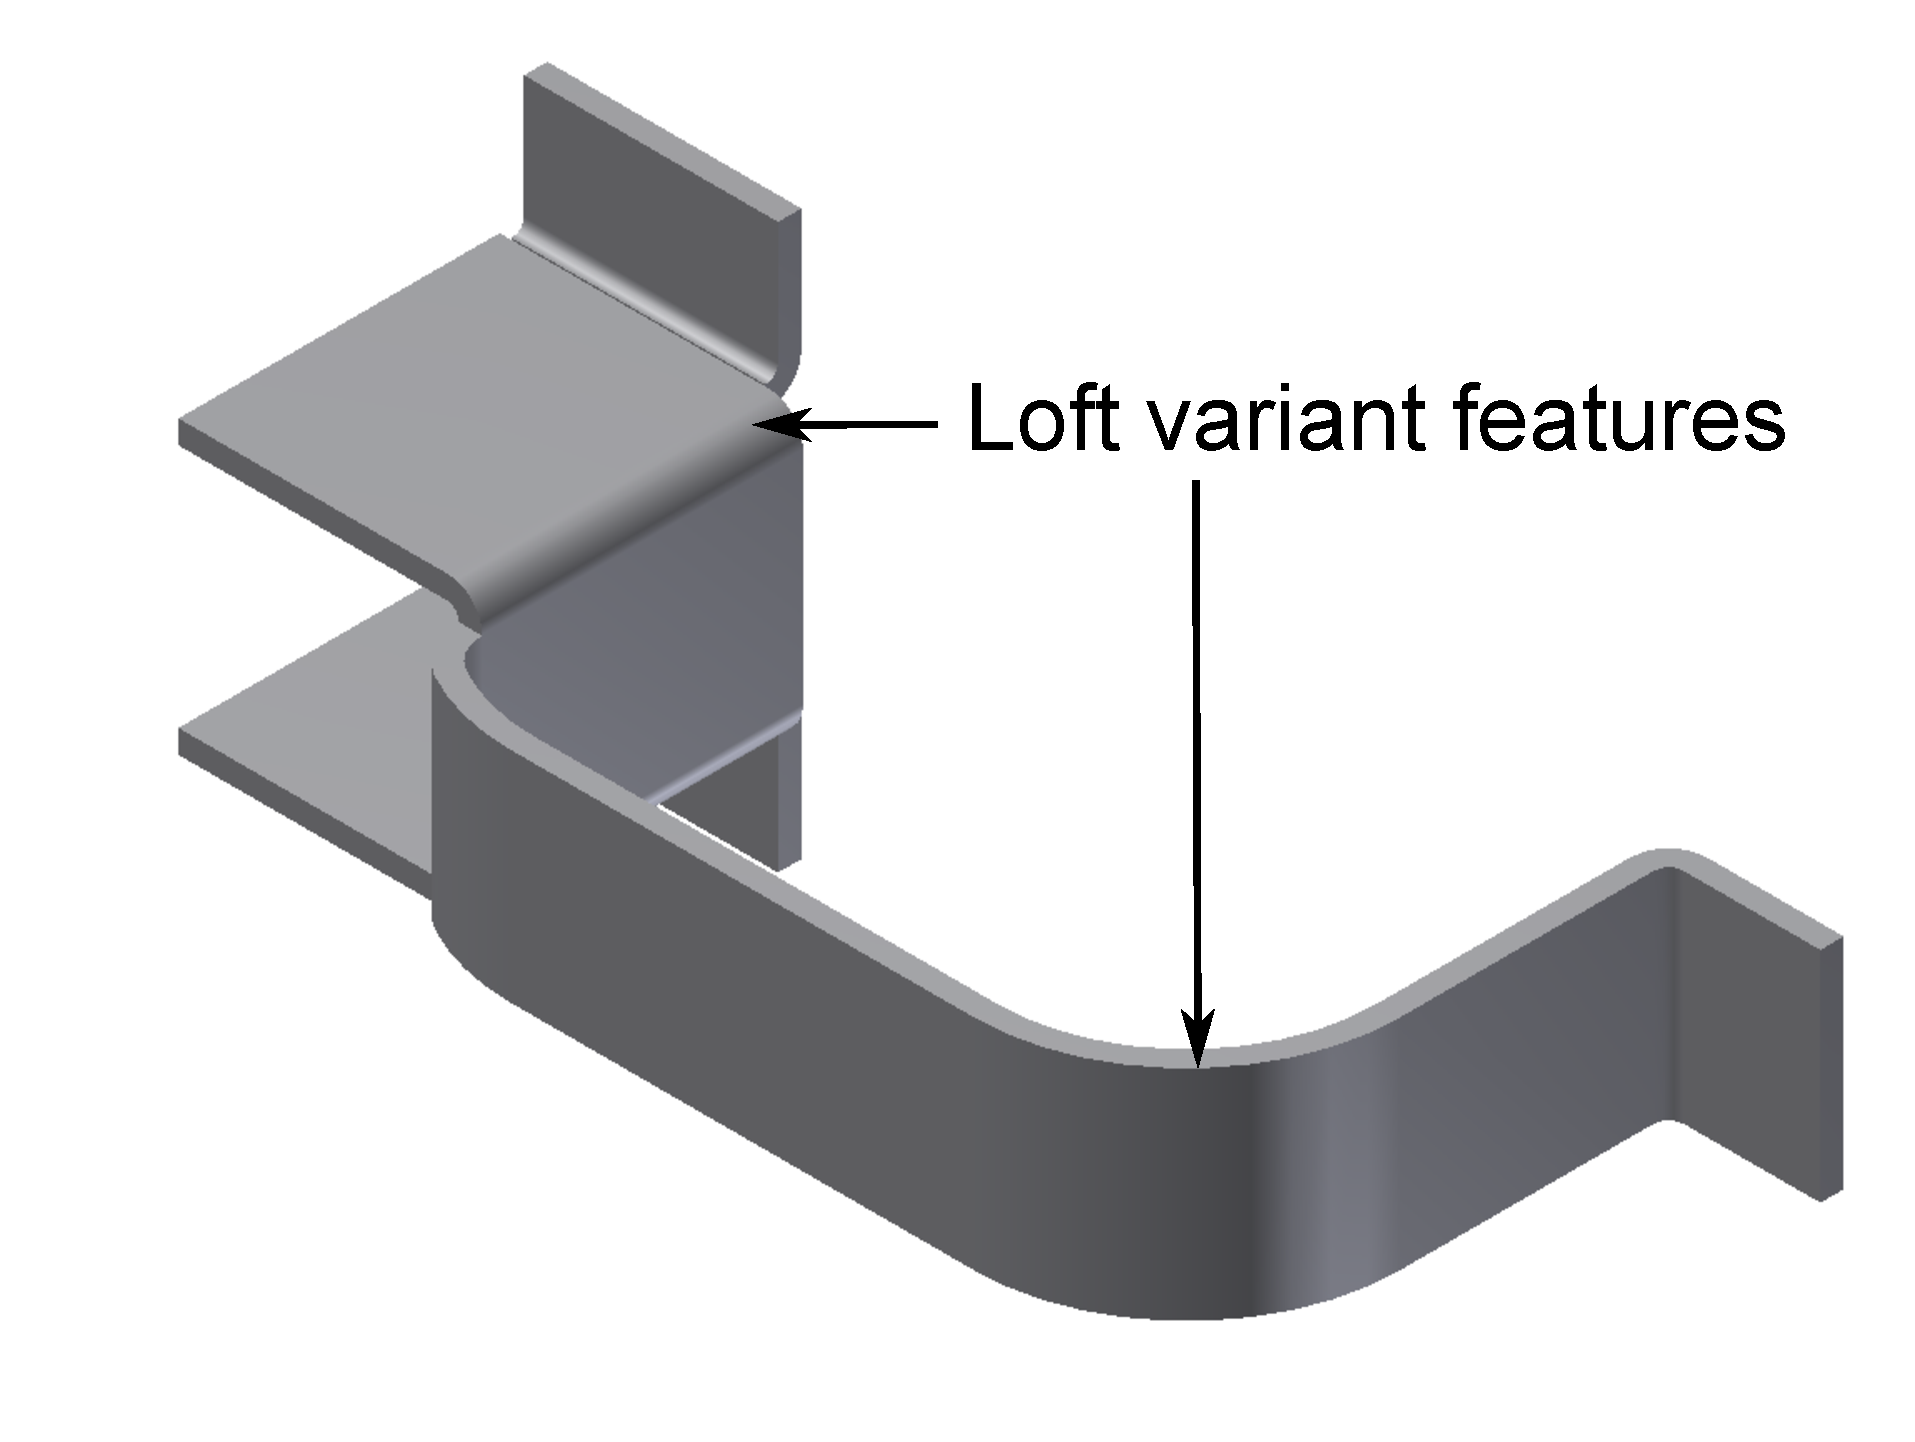
\includegraphics[width=0.45\linewidth,valign=t]{../Common/images/DecompBracketInput_2}}
\subfloat[Feature Based Partitioning]{\label{fig:midsurfcelljoin:cd}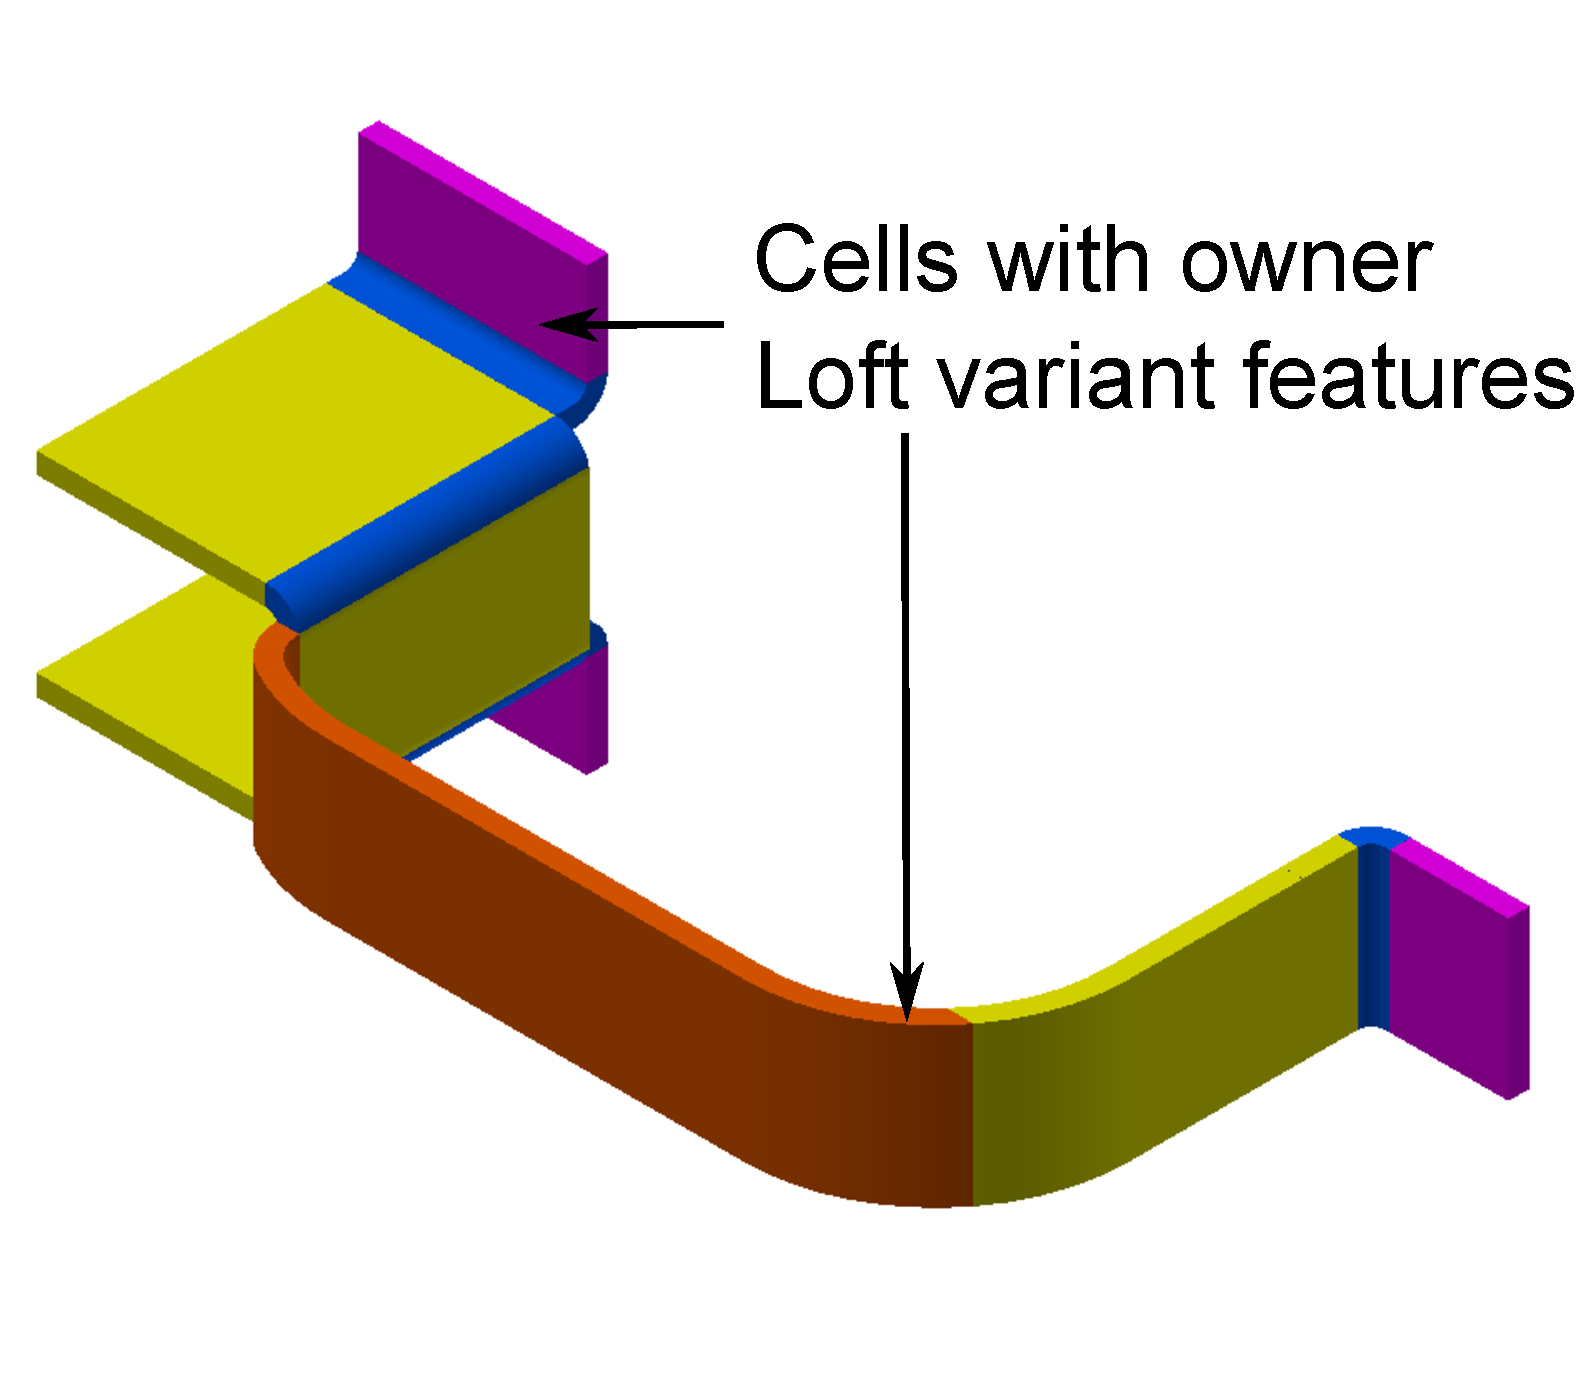
\includegraphics[width=0.38\linewidth,valign=t]{../Common/images/DecompositionBracketOutputPart_2}}\qquad
\caption{Feature-based Cellular Decomposition}
\label{fig:midsurfcelljoin:fbcd}
\end{figure}

%%\bigskip



 Salient features of the proposed FBCD compared to the traditional cellular decomposition approaches are:

\begin{itemize}[noitemsep,topsep=2pt,parsep=2pt,partopsep=2pt]
\item Traditional cellular decomposition works on the B-rep solid model with techniques such as Convex partitioning (CEP), whereas FBCD, as proposed here, works on the feature based CAD model.
\item Cells in FBCD are assigned with the owner feature, but not so in the traditional cellular decomposition. Owner feature information is useful to certain algorithms like Hexahedral meshing~\cite{Wu2014} and also to the present research work for computing midsurface patches. \todo{Review comment: Ok, but how it is beneficial. [ADDED]}
\item In FBCD, the partitioning is not by simply extending all faces beyond the model and using them as cutting tools, rather it resorts to localized partitioning between two interacting features. This makes partitioning effect only in the local zone of interaction, thereby avoiding generation of large number of redundant cells\deleted{\cite{Woo2003a}}.
\end{itemize}
 
The outcome of FBCD is the feature-based cellular topology which is used in the present research to compute the midsurface. 

\subsection{Formation of Feature-based Cellular Topology}\label{sec:midsurfcelljoin:fbct}

FBCT represents a feature based CAD model as a connected set of cells with owner features. Two cells do not overlap volumetrically. Any two adjacent cells are separated by fully overlapping cell-faces.

\begin{figure}[!h]
\centering     %%% not \center
\subfloat[Original Model]{\label{fig:midsurfcelljoin:Lcells}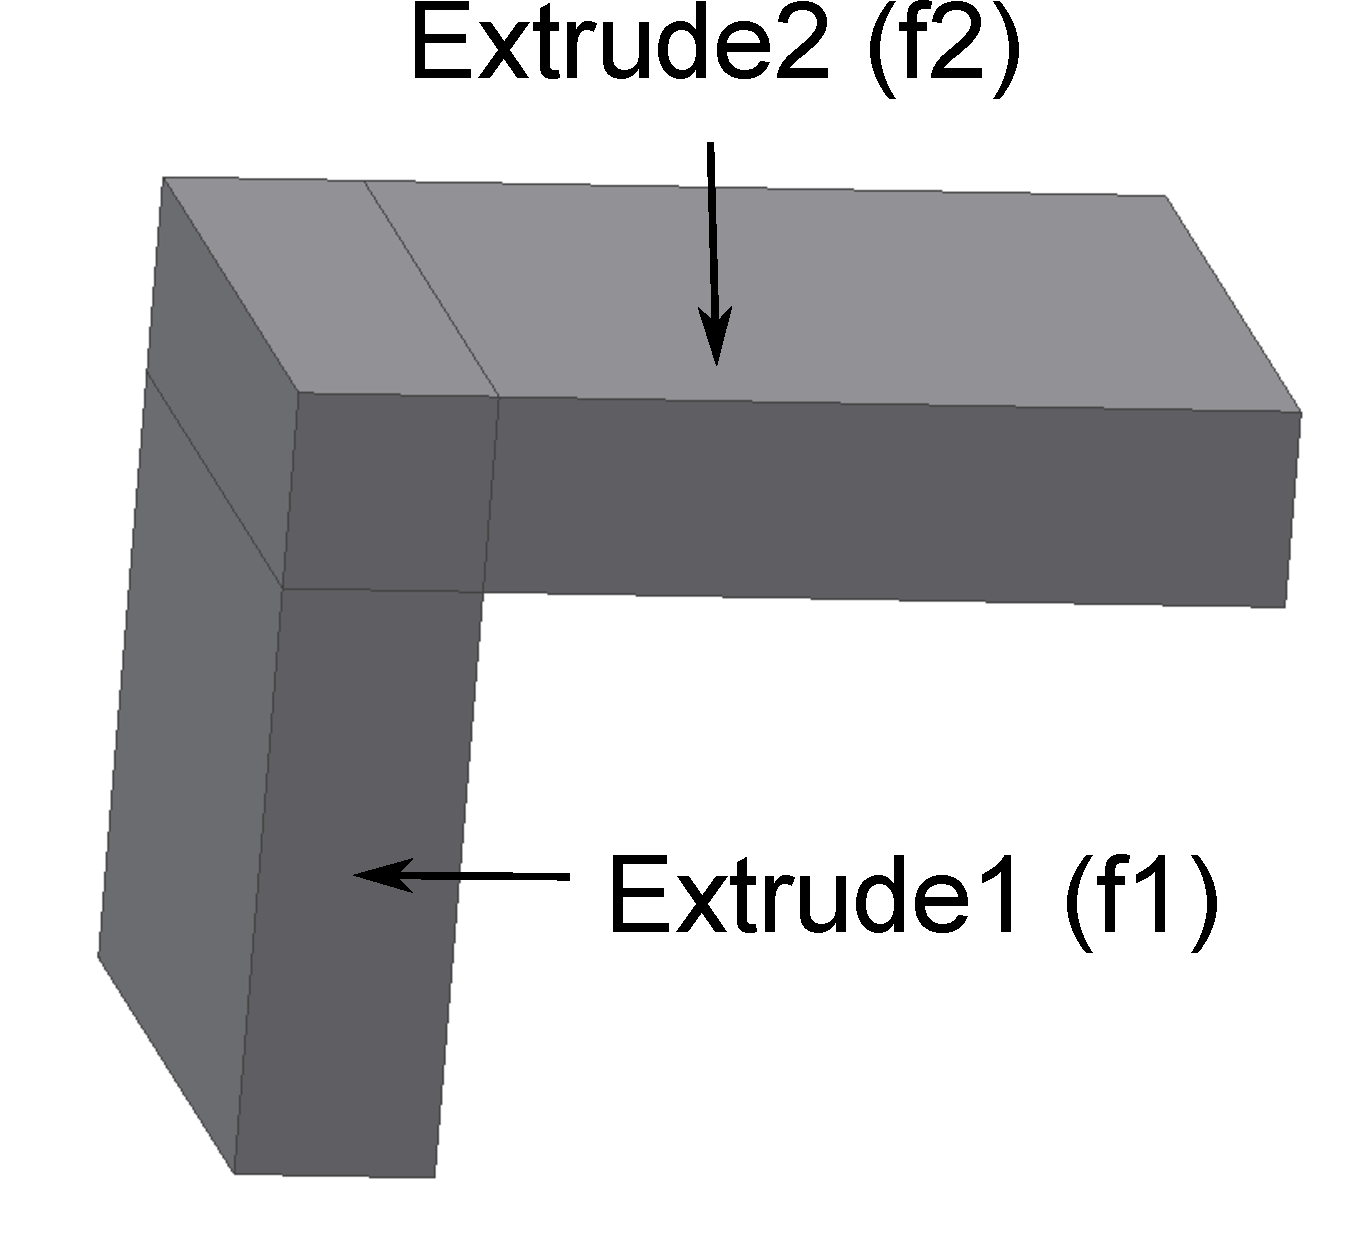
\includegraphics[width=0.3\linewidth,valign=t]{../Common/images/InventorLCells.pdf}} \hfill
\subfloat[Schematic Model]{\label{fig:midsurfcelljoin:twofeat}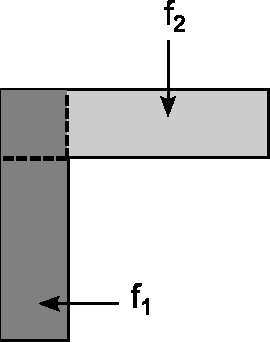
\includegraphics[width=0.22\linewidth,valign=t]{../Common/images/FeatureInteractionMergedPart_1.pdf}} \hfill
\subfloat[FBCT]{\label{fig:midsurfcelljoin:featinteract}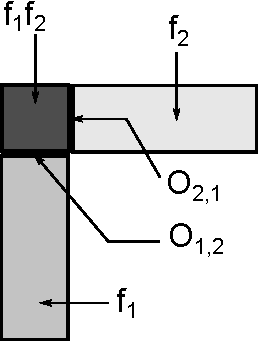
\includegraphics[width=0.21\linewidth,valign=t]{../Common/images//FeatureInteractionMergedCells_1.pdf}}
\caption{Feature-based Cellular Topology}
\label{fig:midsurfcelljoin:fbcd}
\end{figure}

\todo{Review comment: Separate the figure. [MOVED SHEET METAL MODEL BEFORE IN FBCD]}

Figure \ref{fig:midsurfcelljoin:Lcells} shows a representative case, schematically as Figure \ref{fig:midsurfcelljoin:twofeat}, where two features $f_1$ and $f_2$ are interacting. 
\deleted{Interaction can have full or partial volumetric or surface overlaps.} 
\todo{Review comment: I suggest figure showing partial, full, no overlap. [DELETED THE AMBIGUOUS LINE. FBCD RESULTS ONLY IN FULL OVERLAPS. SO NO FIGURE NEEDED]}	
Figure \ref{fig:midsurfcelljoin:featinteract} shows that FBCD decomposes model having features $f_1$ and $f_2$ in such a way that a common cell, with owners $f''_1f''_2$, is formed. Remaining portion of $f_1$ and $f_2$ are termed as $f'_1$ and $f'_2$ respectively.  Overlapping faces are denoted as $O_1$ and $O_2$, where $O$ denotes ``Overlap'' and $_1$ and $_2$ are the ids of instances. 
\todo{Review comment:  Drop this. [DONE]}
\deleted{Thus, now, the cells do not overlap volumetrically [$O_{i,j}^3 = 0$] (meaning, Overlap between cells $_i$ and $_j$ which is of dimensions $^3$, meaning, volumetric), but may overlap at faces [$O_{i,j}^2$] (meaning, Overlap between cells $_i$ and $_j$ which is of dimensions $^2$, meaning surface-wise) fully and not partially, denoted as [ $C_i \cap C_j = 0| O_{i,j}^2$] (meaning, Intersection $\cap$ of cells $C_i$ and $C_j$ is either nothing or full-surface, but not partial).}

In the present research work as the FBCT is generated by decomposing $\mathcal{ABLE}$ features, the owner features of the cells are the $\mathcal{ABLE}$ features, i.e. Loft equivalents. Thus FBCD essentially decomposes the Loft feature tool bodies.

During each decomposition of the original Loft feature's tool body, its corresponding Loft parameters get split. Loft has two parameters, a $profile$ and a $guide-curve$. Decomposition can happen across any or both of these. Remaining parameter ranges are stored in the Loft features for each respective cells.

%%\bigskip


  \begin{figure}[!h]
\centering     %%% not \center
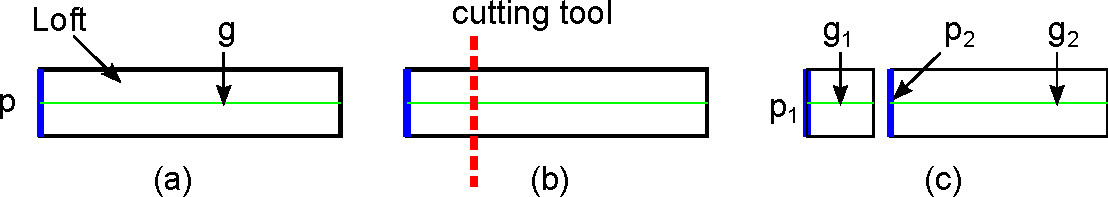
\includegraphics[width=0.75\linewidth,valign=t]{../Common/images/loftbeforecdsweep}
\caption{Loft Feature Partitioning}
\label{fig:midsurfcelljoin:loftbeforecdsweep}
\end{figure}

%%\bigskip


%%
%%
%%\begin{figure}[!h]
%%\centering     %%% not \center
%%\subfloat[Original Part]{\label{fig:midsurfcelljoin:loftbeforecd}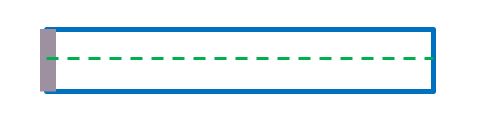
\includegraphics[width=0.3\linewidth,valign=t]{../Common/images/loftbeforecd}}
%%\subfloat[Feature Partitioning]{\label{fig:midsurfcelljoin:loftcd}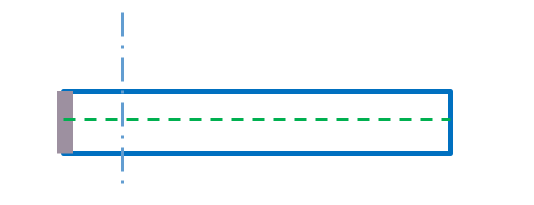
\includegraphics[width=0.33\linewidth,valign=t]{../Common/images/loftcd}}\qquad
%%\subfloat[Features Separation]{\label{fig:midsurfcelljoin:loftseparate}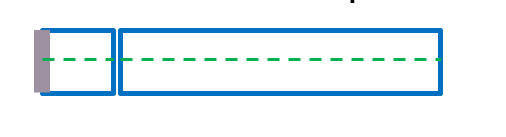
\includegraphics[width=0.3\linewidth,valign=t]{../Common/images/loftseparate}} \qquad
%%\caption{ Loft Splitting and parameter adjustments}
%%\label{fig:midsurfcelljoin:loftfbcd}
%%\end{figure}

\todo{Review comment: change figure to flange like. [NOT DONE, AS TANGENT CONTINUOUS SHAPES ARE NOT CUT BY FBCD BUT ONLY THOSE HAVING CONCAVE EDGES]}

Figure \ref{fig:midsurfcelljoin:loftbeforecdsweep}a shows a single Loft feature getting decomposed and is represented by profile $p$ and guide curve $g$. In this particular case cutting is happening on the guide curve $g$. Figure \ref{fig:midsurfcelljoin:loftbeforecdsweep}b shows the cutting geometry used to decompose. Figure \ref{fig:midsurfcelljoin:loftbeforecdsweep}c shows the outcome of FBCD, i.e. two cells, with profiles $p_1$ and $p_2$ along with the guide curves $g$ cut into two $g_1$ and $g_2$, respectively.  For both the cells, profile $p$ is same as before but the parameter ranges of $g$ are different, e.g the first cell has $p, g_{0,0.3}$, whereas the second cell has $p, g_{0.3,1}$. Similar cutting can happen across $profile$ as well, where the guide-curve ($g$), may remain uncut.

%Following are the observations of FBCD of the Loft feature volumes:
%\begin{itemize}[noitemsep,topsep=2pt,parsep=2pt,partopsep=2pt]
%\item All cells are of Loft type (profiles as thick blue line, guide as red line) (Figure \ref{fig:midsurfcelljoin:loftbeforecdsweep}).
%\item The Splitting plane, creates the Interface  (Figure \ref{fig:midsurfcelljoin:loftbeforecdsweep}).
%\item Interface has two adjacent sides. It removes existing midsurface patches and creates new shapes connecting midsurfaces from interface-faces (Figure \ref{fig:midsurfcelljoin:loftseparate}).
%\item It can store Loft parameter range on each of its side. Left side ($p, d_{0,0.3}$) and Right side ($p, d_{0.3,1}$). Similar splitting can happen for Profile as well, where guide-curve ($d$), remains constant. Both cells are owned by the same Loft.
%\end{itemize}

Following subsection elaborates process of populating a graph of the FBCT cells.

\subsection{Formation of Feature-based Cellular Graph}

FBCT has, say $n$ cells, each assigned with a Loft owner-feature. A cell adjacency graph [CAG, $G(n,e)$] is formed with $n$ nodes, each pointing to and representing a cell. Figure \ref{fig:midsurfcelljoin:featgraph} shows the CAG of simple cells-configuration of a ``L'' shaped part. Node $n_1$ corresponds to a cell, with owning feature $f'_1$, whereas node $n_3$ corresponds to the cell with owning feature $f'_2$. The common cell owned by $ f''_1f''_2$ is represented by node $n_2$. Note that the terms ``node'' and ``cell'' are used synonymously hereafter, unless specified otherwise. Each boundary face between two nodes is represented by an edge ($e$). Edge $e_{12}$ corresponds to the overlapping face $O_1$, where as  edge $e_{23}$ corresponds to the overlapping face $O_2$. 

%%\bigskip

\begin{figure}[!h]
\centering 
\begin{minipage}[h]{0.3\linewidth} 
\includegraphics[width=\linewidth]{../Common/images/FeatureInteractionGraph.pdf}
\end{minipage} \hfill
\begin{minipage}[h]{0.22\linewidth} 
\centering \includegraphics[width=\linewidth]{../Common/images/CellDecompExample.pdf}
\end{minipage}\hfill
\begin{minipage}[h]{0.38\linewidth} 
\begin{itemize}[noitemsep,topsep=2pt,parsep=2pt,partopsep=2pt]
\item $n_1 = sCell_1= f'_1$
\item $n_2 = iCell_1 = f''_1f''_2$
\item $n_3 = sCell_2 = f'_2$
\item $e_{12} = O_1$
\item $e_{23}= O_2$
\end{itemize}
\end{minipage}
\caption{Feature-based Cellular Graph}
\label{fig:midsurfcelljoin:featgraph}
\end{figure}

%%\bigskip

%Each node in CAG represents a cell from FBCT with owning-feature(s) assigned to each of them. \deleted{A cell body has three dimensions, the two sides of the aligned bounding box of the sketch and the length of the guide curve (say, $d_1,d_2,d_3$). FbCD results in $n$ cell-bodies with owning-feature(s) assigned to each of them.} A cell adjacency graph [CAG, $G(n,e)$] is formed with the $n$ nodes, each representing a cell-body. For each face-overlap between two nodes, an edge ($e$), having two nodes ($n$) attached on either end, is created in the CAG

Following section elaborates classification of the cells, which helps in delegating specific tasks to each in the proposed approach of computation of the midsurface.

\subsection{Classification of Cells} \label{sec:midsurfcelljoin:classfication}

Based on the expectations from midsurface shown in Figure~\ref{fig:introduction:midsurfaceexptations} in Chapter~\ref{ch:Survey}, it can be seen that, the model can be conceptually divided into two portions with different functionalities, viz midsurface patches generating portions and midsurface patch joining portions. When this observation is mapped to CAG shown in Figure~\ref{fig:midsurfcelljoin:featgraph}, it is clear that nodes $n_1, n_2$ are patch generating nodes and $n_2$ is a patch joining node. Thus, nodes are classified as $patch$ nodes and $junction$ nodes respectively. This classification is done based on the graph topology and characteristics of the owner feature parameters of the cells, these nodes point to.

 \begin{figure}[!h]
\centering     %%% not \center
\includegraphics[width=0.3\linewidth,valign=t]{../Common/images/InventorCell.pdf}
\caption{Cell with Dimensions}
\label{fig:litsurvey:celldim}
\end{figure}

Cells are classified as solid cells ($sCell$s, pointed by $patch$ nodes) and interface cells ($iCell$s, pointed by $junction$ nodes). Figure~\ref{fig:litsurvey:celldim} shows a cell with dimensions. Its classification rules are as follows:

%%\bigskip




%%\bigskip


\begin{mydef}
\label{def:midsurfcelljoin:scell}
Solid cell ($sCell$) is a cell-body with only one of its dimensions ($d_1$) less than the threshold-factor ($t$) times any of the other two dimensions ($d_2, d_3$), denoted as  $d_1 < t \times d_2 \quad \&  \quad d_1 < t \times d_3$. %node representing a Thin cell-body and with 0/1 incident edge.% any adjacent node with owning-feature as ``Loft'' and is not an $iCell$.
\end{mydef}
\begin{mydef}
\label{def:midsurfcelljoin:icell}
Interface cell ($iCell$) is a cell-body with minimum two dimensions ($d_1,d_2$) less than the threshold-factor ($t$) times of the maximum dimensions ($d_3$), denoted as  $d_1 < t \times d_3 \quad \&  \quad d_2 < t  \times d_3$. %node with 2/more incident edges. %and has respective overlapping faces ($O_1,O_2$) adjacent to each other.
\end{mydef}


In Figure \ref{fig:midsurfcelljoin:featgraph}, nodes $n_1$ and $n_3$ point to cells which are solid cells ($sCell$), whereas node $n_2$ points to cell which is interface cell ($iCell$).  

The fundamental rule of midsurface computation is stated by Def.~\ref{def:midsurfcelljoin:midsurfrule} as:

\begin{mydef}
\label{def:midsurfcelljoin:midsurfrule}
$sCell$ computes the midsurface patches, whereas the  $iCell$ connects all the midsurface patches incident on them
\end{mydef}			

Advantage of the CAG representation is that, it is easier to classify nodes based on cell characteristics and delegate specific computational work to each using generic rules. \deleted{Thus, the proposed research does not need to enumerate specific heuristic rules used for specific connection types} Another advantage is that, as the problem space has been decomposed into manageable sub-problems\deleted{, thereby complexity of the original problem becomes irrelevant. However large or complex the input CAD model may be,  decomposed cells can be handled, one by one, deterministically}. 

Following sections elaborate the work delegated as per Def.~\ref{def:midsurfcelljoin:midsurfrule} to the classified cells.

\section{Generating Midsurface Patches from Solid Cells}
\label{sec:midsurfcelljoin:scell}

This section presents an algorithm for computing a midsurface patch from a solid cell ($sCell$). The patch is generated based on the profile $p$ and the guide curve $g$  of the owner loft feature of the $sCell$. Depending on the aspect ratio of the $sCell$, midsurface patch computation varies. Two method are available, namely Midcurve based and Offset based. Midcurve based method is suitable wither the profile is ``thin'' and has a long guide curve, whereas the offset method is suitable where guide is shorter compared to the profile. Thus the input $sCell$ is first classified and the accordingly midsurface patch computation method is chosen. Thus, the $sCell$ is classified into long guide, short guide and equal guide.

%%\bigskip

  \begin{figure}[!h]
\centering     %%% not \center
\includegraphics[width=0.75\linewidth,valign=t]{../Common/images/typesofscell_1.pdf}
\caption{Types of $sCell$s}
\label{fig:midsurfcelljoin:typesofscell}
\end{figure}

%%\bigskip

Figure~\ref{fig:midsurfcelljoin:typesofscell}a shows an Extrude feature (a Loft equivalent) having a profile and a guide curve where guide is far shorter than the size of the profile. This case is called as ``Short Guide''. Profile, being a 2D entity, its comparison with 1D guide curve can not be done directly. So, perimeter of the profile with some scaling factor, is compared with the length of the guide. This size comparison determines the `thinness' of the $sCell$.  As mentioned in Section \ref{sec:survey:intro}, though the criterion for ``thinness'' depends on the domain, $thinness = 2$ is considered for the present research. Figure~\ref{fig:midsurfcelljoin:typesofscell}b shows a similar Extrude but which is built by extruding smaller profile along longer guide direction. This case is called as ``Long guide''. Figure~\ref{fig:midsurfcelljoin:typesofscell}c shows case of Extrudes whose profile and guide sizes are similar. These cases are called as ``Equal Guide'' and the cells as ``thick cells''.

% \added{Comparison is done between $sketch_{size}$ and $guide_{size}$. Symbol $\ll$ suggests that length of the sketch has to be far less than length of the guide, for the {\bf $\mathcal{L}$} to get qualified for ``Thin Sketch'' (elaborated below) method of computing midsurface. $sketch$ being a 2D entity, its size (i.e. area) can not be compared directly with the size (i.e. length) of the $guide$. So, the present research takes summation of sketch curve lengths as the parameter denoting $sketch_{size}$, whereas $\ll$ is taken as factor of 2, meaning, $sketch_{size}$ has to at-least 2 times less that the $guide_{size}$.}

Based on the above mentioned type of $sCell$s,  different midsurface patch generation approaches are used, as described below: 

\begin{figure}[h]
\centering \includegraphics[scale=0.62]{../Common/images//MidsurfSmallProfile_3.pdf} 
\caption{Long Guide $sCell$}
\label{figure_MidsurfSmallProfile_2}
\end{figure}



\begin{itemize}[noitemsep,topsep=2pt,parsep=2pt,partopsep=2pt]

\item {\bf Long Guide $sCell$}: {\em Midcurve} is extracted from the {\em profile} and swept along the {\em guide} to generate the midsurface patch.

%%\bigskip


%%\bigskip

Figure~\ref{figure_MidsurfSmallProfile_2} shows a solid cell having a profile, a guide, a midcurve computed and the midsurface patch generated. Details of computation of the midcurve are presented in the next section.

\item {\bf Short Guide $sCell$} : The {\em profile} face itself is {\em offseted} along half {\em guide} length. {\em Midcurve} is not computed  in this case.  

\item {\bf Equal Guide $sCell$}:  This is a thick cell and thus midsurface patch is not generated for it. During midsurface patch joining phase, relevant thick cells may participate as patch joining cells.

\end{itemize}

\todo{Review comment: I suggest first explain the simple part ie.e generating midsurface by simply offsetting the faces...[ADDED DETAILED EXPLANATION]}

Algorithm~\ref{alg:midsurfcelljoin:MidsurfsCell} describes the midsurface patch generation process in a pseudo-code. 

\bigskip


		\begin{algorithm}[H]
		\caption{sCell Midsurface Patch Computation}
		\label{alg:midsurfcelljoin:MidsurfsCell}
		\begin{algorithmic}[1]
			\REQUIRE $sCell$
			%\ENSURE $size(sCell \rightarrow owning-feature(s)) = 1$
			\STATE $f = sCell \rightarrow owning\_feature()$
			\STATE $p = f \rightarrow get\_profile()$
			\STATE $g = f \rightarrow get\_guide()$
			%\STATE $is\_thin\_profile = \sqrt{Area(profile)} < threshold \times length(guide)$ 
			\IF{$is\_long\_guide(p,g) == true$}
				\STATE $m^1 = p\rightarrow compute\_midcurve()$
				\STATE $m^2 = sweep(m^1 ,g)$
			\ELSIF{$is\_short\_guide(p,g) == true$}
				\STATE $m^2 = offset(p ,g/2)$
			\ENDIF
		\end{algorithmic}
	\end{algorithm}

\bigskip




%%\bigskip

Steps for the same are elaborated below:

\begin{enumerate}
[noitemsep,topsep=2pt,parsep=2pt,partopsep=2pt]
\item Owner feature is queried from the input $sCell$. From the owner feature, which is a Loft-equivalent, its profile and guide are extracted (Algorithm~\ref{alg:midsurfcelljoin:MidsurfsCell} lines: 1-3).
\item Based on the relative size of profile with respect to guide, the $sCell$ is checked if it is Long-guide or a Short-guide cell.
\item If it is a Long-guide case, then midsurface patch is computed by ``midcurve' method.
\item Midcurve from the profile is computed and it is swept along the guide to create a midsurface patch (Algorithm~\ref{alg:midsurfcelljoin:MidsurfsCell} lines: 5-6).
\item If the cell is of Short-guide type then ``offset'' method is used.
\item The profile face is offseted at half the distance of the guide to compute the midsurface patch (Algorithm~\ref{alg:midsurfcelljoin:MidsurfsCell} line: 8).
\end{enumerate}

	
Figure \ref{fig:midsurfcelljoin:scells} shows the outcome of this midsurface patch generation module with a sample ``L'' shaped model. FBCD decomposed it into 3 cells, out of which 2 are $sCell$s. The first picture shows schematic diagram of the two $sCell$s having midsurface patches generated in each of them. The cell in between is an $iCell$, so it is not handled in this module. The second picture shows the same scenario as a 3D view, showing the two midsurface patches.

	\begin{figure}[!h]
	\centering     %%% not \center
	\subfloat[Patches, 2D view]{\label{fig_patches2d}\includegraphics[width=0.3\linewidth]{../Common/images/MidsurfPatches_2.pdf}} \quad
	\subfloat[Patches, 3D view]{\label{fig_patches3d}\includegraphics[width=0.3\linewidth]{../Common/images/sCellMidsurfs3d}}
	\caption{Midsurface Patches } %%%%%%%% ADD (\{citeYogeshIITG2014}) LATER
	\label{fig:midsurfcelljoin:scells}
	\end{figure}

Once done, all the $sCell$s are filled with the midsurface patches and are ready to get connected in $iCell$s, which is eleborated in Section \ref{sec:midsurfcelljoin:icell}.

Following section describes the proposed approach of generating midcurve from Loft feature's profile, needed in case of ``Long Guide'' $sCell$ case.

\subsection{Generation of Midcurves from Profile} \label{sec:midcurve}
%\section{Introduction}
This section presents a proposed approach of computing midcurve of a given profile, in case of Long-Guide $sCell$. The owner feature of this cell, the Loft, has longer guide curve compared to size of its profile. It needs to be noted that in feature based CAD paradigm, sketch consists of one or more profiles. There is one outer profile which represents the boundary of the sketch and the remaining profiles represent inner holes in the sketch. When there is only one i.e. outer profile, the terms sketch and the profile are used synonymously.

\deleted{The way a midsurface is dimension reduction of a thin solid,  a midcurve is dimension reduction of a profile. }Midcurve is a curve, which lies midway of a profile\deleted{, representing the profile}. \deleted{Applications such as shape matching, shape retrieval, animations, etc, need a lower dimension representation such a midcurves,  as not only they are faithful representation of the input shape but also have lower data due to lower dimension. Generically, a skeleton is such an entity which represents the input shape in the lower dimension.} It, being lower in dimension than the input shape, applications like pattern recognition, approximation, similarity estimation, collision detection, animation, matching and deformation can be performed efficiently on it compared to them done on the original input shape. 

\todo{Review comment: Substantiate with figure. [DONE]}

%%\bigskip

\begin{figure}[h]
\centering \includegraphics[width=0.45\linewidth]{../Common/images/midcurveexamples_1.pdf} 
\caption{Examples of Midcurves}
\label{fig_midcruveexamples}
\end{figure}

%%\bigskip

Figure~\ref{fig_midcruveexamples} shows two examples. Figure~\ref{fig_midcruveexamples}a shows a ``Y'' profile, with its midcurve whereas Figure~\ref{fig_midcruveexamples}b shows a ``L'' profile with its midcurve. Note that, both midcurves are one dimension less and lie midway of the respective profiles.

%%Some representative usages are:
%%\begin{itemize}
%%[noitemsep,topsep=2pt,parsep=2pt,partopsep=2pt,leftmargin=*]
%%\item \textbf{Midsurface}: For Sweep based volumes, Midsurface is nothing but  sweeping of the Midcuves of the Sketch
%%
%%\raisebox{-.9\height}{\includegraphics[width=0.5\linewidth]{..//Common/images/MidsurfSmallProfile.pdf}}
%%
%%\item \textbf{Pattern Matching}: Instead of finding similarity between 2D profiles, it is easier to do the same with Midcurves.
%%
%%\item \textbf{Shape Retrieval}: For retrieving particular 2D shape from the database, Midcurve can be used as signature/meta-data, instead of string/tag based, making selection more deterministic.
%%\end{itemize}

Most of the midsurface generation approaches reviewed in Chapter~\ref{ch:Survey} in Section~\ref{sec:survey:observationsformal} are applicable to midcurve generation as well. Only difference is, instead of a 3D solid model as input for midsurface generation, a 2D profile is the input for midcurve generation. Approaches such as Medial Axis Transform (MAT),  Chordal Axis Transform (CAT), Thinning etc. are used to compute, a generic curve form, known as medial curves. Midcurve is one specialization of the medial curve. Figure~\ref{fig:litsurvey:midcurve}b had shown midcurve output where spurious branches have been replaced by two extensions forming a continuous line, thus mimicking the original shape.

Ramanathan~\cite{Ramanathan2004} states that no formal definition exists for either midcurve or midsurface. He attempted to define midsurface semi-formally as seen in Definition~\ref{def:midsram}. Similarly midcurve can also be defined as:

\begin{mydef}\label{def:midcurve}
Midcurve is an aggregation of curve segments (where each segment corresponds to a pair of nonadjacent edges in the object that are closest to each other) that form a closed and connected set and that satisfy homotopy
\end{mydef}

Review of the reported approaches of computing medial curves is presented in Chapter~\ref{ch:Survey} in Section~\ref{sec:survey:observationsformal}. 
%%
%%Following is summary of some of the salient observations:
%%\begin{itemize}[noitemsep,topsep=2pt,parsep=2pt,partopsep=2pt]
%%	\item Biggest strength of formal approaches like MAT is that it can be computed of any shape, thick or thin. Being formally defined, the converse or reversal process, meaning ``given a MAT compute the original shape'', is possible.
%%	\item Major drawback of MAT, Thinning methods is that it creates unnecessary branches and its shape is smaller than the original corresponding faces.
%%	\item  MAT based approaches also suffer from robustness problem. A slight change in base geometry forces re-computation of MAT and the results could very well be different than the original.
%%	\item Although MAT approaches have been around for decades and are fairly mature, its usage in midcurve generation is still very complex and difficult to ensure appropriate topology.
%%	\item The major limitation of CAT approach is that mesh has to be generated beforehand. Creating constrained, single layer meshes on complicated 2D profiles are, at times, difficult.
%%	\item Thinning approaches are based on split events of the straight line skeleton gives counter-intuitive results if the polygon contains sharp reflex vertices.
%%	\item In Parametric approach, the two input curves or surfaces may not be in one-to-one form. In such cases maintaining continuity can be challenging.
%%	\item Quality of surface generated by parametric approach depends on the sampling done to compute the midpoints.
%%\item Midcurve by profile decomposition approach is not used widely. The decomposition can result in large number of redundant sub-shapes making it ineffective and unstable for further processing.
%%\end{itemize}
%%
It suggests to avoid formal methods such as MAT, CAD, Thinning and Parametric, for computing midcurve as they need heavy post-processing to remove unwanted curves. The heuristic method of decomposition, which has been error prone and inefficient so far, appears promising in case of profile decomposition if enhancements can be proposed.

Following section takes a closer look at some of the existing profile decomposition approaches. After that, existing midcurve generation approaches based on profile decomposition are also reviewed.


\subsection{Related Work}

Many approaches assume the input profile to be of simple polygon type, meaning, all the profile curves are linear and non-intersecting. The polygonal profile is assumed to be a set of connected lines end to end and closing the loop.

Keil~\cite{Keil94} presented an approach based on convex partitioning, i.e. partitioning polygon at concave vertices, with an intent of making sub-polygons, convex. Figure~\ref{fig_keil} shows how his approach finds all possible ways to remove concavity of vertices and then takes the one that requires fewest diagonals.

Lien et. al.~\cite{Lien2004} decomposed polygons 'approximately' based on iterative removal of the most significant non-convex feature. 

Bayazit~\cite{Bayazit} presented a polygon decomposition method based on Concave (Reflex) angle partitioning. Figure~\ref{fig_bayazit} shows the partitioning at specific concave vertices. Although the output was far better than if usual meshing had been employed, the drawback was it left out some corner cases giving more than necessary divisions.

%%\bigskip

	\begin{figure}[!h]
	\centering     %%% not \center
	\subfloat[Keil~\cite{Keil94}]{\label{fig_keil}\includegraphics[width=0.4\linewidth]{../Common/images/keilwnames.pdf}} \quad
	\subfloat[Bayazit~\cite{Bayazit}]{\label{fig_bayazit}\includegraphics[width=0.4\linewidth]{../Common/images/bayazit}}
	\caption{Polygon Decomposition Methods} %%%%%%%% ADD (\{citeYogeshIITG2014}) LATER
	\label{fig:litsurvey:polydecomp}
	\end{figure}
	
%%\bigskip

%%Below is the summary of some of these relevant profile decomposition approaches:
%%
%%\csvreader[longtable=|p{0.17\linewidth}|p{0.11\linewidth}|p{0.15\linewidth}|p{0.2\linewidth}|p{0.17\linewidth}|p{0.17\linewidth}|,
%%    table head=\toprule \bfseries Author & \bfseries Input& \bfseries  Method & \bfseries  Approach& \bfseries  Advantages& \bfseries  Limitations \\ \midrule \endhead,% \bottomrule \endfoot,
%%  late after last line=\\\bottomrule,
%%  before reading={\catcode`\#=12},after reading={\catcode`\#=6},    
%%    late after line=\\\hline]%
%%{../DocsSources/litsurvey_polydecomp.csv}{Author=\Author, Input=\Input, Method=\Method, Approach=\Approach, Advantages=\Advantages ,Limitations=\Limitations}%
%%{\Author  & \Input&  \Method &\Approach & \Advantages & \Limitations}%
%%
%%Thus, review of the approaches suggests that the polygon decomposition rules depend on the application context, accuracy, characteristics  and aspect ratio of the sub-polygons. Judicious selection of these parameters will decide the applicability to the problem being solved.
%%
%%Following are some of the midcurve generation approaches based on profile decomposition:
%%
%%% Choi~\cite{Choi1997} subdivided the planar region with holes into smaller simply connected planar sub regions that overlap only at the joints where subdivision occurs. Approximated medials based on Bezier-Bernstein curves are computed for individual sub-regions. 
%%% Decomposition of planar shapes  into regular (non-intersecting) and singular (intersecting regions) and its application to skeletonization has been widely researched~\cite{Rocha99} as well.
%%% 
Rocha~\cite{Rocha98}~\cite{Rocha99} presented skeletonization approach for images which primarily worked on vertices. Figure~\ref{fig_rocha} shows how the sub-shapes computed mid-segments which were joined at the connections. Although this approach could address many shapes, it lacked comprehensive coverage and did not do very well for simple joints like T and L

%%\bigskip

\begin{figure}[h]
\centering \includegraphics[width=0.5\linewidth]{../Common/images/rocha} 
\caption{Midcurve Computation after Polygon Decomposition}
\label{fig_rocha}
\end{figure}

%%\bigskip

%Bag~\cite{Bag2011} computed mid-segments for character image which preserve the local characteristics.
% 
% Below is the summary of the relevant midcurve computation approaches:
% 
%\csvreader[longtable=|p{0.17\linewidth}|p{0.11\linewidth}|p{0.2\linewidth}|p{0.2\linewidth}|p{0.17\linewidth}|p{0.17\linewidth}|,
%    table head=\toprule \bfseries Author & \bfseries Input& \bfseries  Medial& \bfseries  Approach& \bfseries  Advantages& \bfseries  Limitations \\ \midrule \endhead,% \bottomrule \endfoot,
%  late after last line=\\\bottomrule,
%  before reading={\catcode`\#=12},after reading={\catcode`\#=6},    
%    late after line=\\\hline]%
%{../DocsSources/litsurvey_midcurvedecomp2d.csv}{Author=\Author, Input=\Input, Method=\Method, Approach=\Approach, Advantages=\Advantages ,Limitations=\Limitations}%
%{\Author  & \Input&  \Method &\Approach & \Advantages & \Limitations}%
%
%\subsubsection{Observations on Midcurve by 2D Decomposition Approaches}

Review of the approaches suggests that the polygon decomposition rules are needed to take into account the application context, accuracy, characteristics  and aspect ratio of the sub-polygons. For the present research work, the midcurve generation needs primitive shaped, thin sub-polygons. Non-primitive, skewed shapes would result in inappropriate midcurves.

Following section proposes midcurve computation approach based on profile decomposition. % method which has improved an existing approach by Bayazit~\cite{Bayazit} to suit the characteristics of sub-polygons needed for computation of midcurve.
\subsection{Proposed Approach for Generating Midcurve}
In previous chapters it is seen that the proposed midsurface computation approach, first simplifies the input model by defeaturing, unifies the feature representation by generalization and then decomposes the simplified model into cells. Cellular topology makes devising generic approach for computing midsurface, easier and deterministic. Similar approach can also be used in computing midcurve from a profile.

Following is the proposed approach for computing midcurve which takes the input profile though similar stages as that of computation of midsurface. 
 
 %%\bigskip

\begin{figure}[h]
\centering \includegraphics[width=0.5\linewidth]{../Common/images/SystemArchitectureMidcurve_2.pdf} 
\caption{Overall Wokflow of Proposed Midcurve Computation}
\label{fig_sysarchmidcurve}
\end{figure}

%%\bigskip

Figure~\ref{fig_sysarchmidcurve} shows the stages which are explained below:

\begin{enumerate} [noitemsep,topsep=2pt,parsep=2pt,partopsep=2pt]
\item Input to this approach is a profile, of a generalized Loft of $\mathcal{ABLE}$ paradigm, who is an owner feature of a $sCell$ for which a midsurface patch is being computed. The profile is typically made up of a variety of curves, such as lines, arcs, splines, etc. joined end-to-end forming closed loops. 
\item During simplification of the profile, the curves are faceted into linear segments. Thus the input profile becomes a polygon. This is termed as ``Polygonization''.
\item Polygon decomposition approach needs a single polygon whereas Loft feature's sketch may have inner profiles representing holes. These inner profiles are connected to outer boundary profile via bridge curves. Thus multiple profiles get converted to single continuous polygon. This is termed as ``Unification''.
\item During decomposition the polygon is split into sub-polygons, called 2D cells.
\item The set of connected 2D cells is used to compute the midcurve.
\end{enumerate}

Amongst the stages shown, Polygonization and Unification are already established techniques. Decomposition and Midcurve Computation are the two areas in which the present research work has contributed. Following subsections elaborate them in details. Input to them is a polygon which is arrived at after the``Polygonization'' and ``Unification'' processes,as  mentioned above. %Thus, the polygon is used as input to the further stages.

% the process of computing a midcurve goes through two phases viz. Decomposition and Midcurve computation. The process of polygon decomposition devised here, is based on an algorithm originally developed by Mark Bayazit~\cite{Bayazit}. He mentions basic rules for decomposition as:
%\begin{enumerate} [noitemsep,topsep=2pt,parsep=2pt,partopsep=2pt]
%\item A polygon can be broken into convex regions by eliminating all reflex vertices.
%\item A reflex vertex can only be removed if the diagonal connecting to it is within the range given by extending its neighboring edges; otherwise, its angle is only reduced.
%\end{enumerate}
%


\subsection{Polygon Decomposition}

Polygon decomposition is the partitioning of polygons into primitive sub-polygons. 
%Polygons come with different types of variations. They can be simple or self-intersecting, with or without holes, concave or convex etc. Although the algorithms presented here can compute midcurves for any simple polygon, but they are most relevant for thin elongated shapes such as alphabets made using Ribbon-like primitives. %For this work, more focus is given on profiles with constant thickness with test cases based on English alphabets. 
Strategy for `where-to-partition' depends on the application's need. Decompositions are done in such a way that minimum number of convex sub-polygons produced or total length of the boundary is minimized, etc. Convex Partitioning is one of the most popular method of polygon decomposition where partitioning happens at vertices having concave angle. Thus, as the concavity at those vertices is removed, after partitioning, the sub-polygons generated are of convex type having all vertices with convex angle. 

 %%\bigskip

\begin{figure}[h]
\centering \includegraphics[width=0.62\linewidth]{../Common/images/convexcgal} 
\caption{Convex Partitioning (Source: CGAL~\cite{cgal})}
\label{fig_cgal}
\end{figure}

%%\bigskip

Figure~\ref{fig_cgal}a shows one of the possible polygon decomposition approaches whereas Figure~\ref{fig_cgal}b shows Convex Partitioning. The present research proposes to go in the direction of Convex partitioning but with an enhanced approach as elaborated below.

%Within the minimum component criterion, the methods are further classified based on whether or not Steiner points (brand new, non polygonal vertices) are allowed. A method devised here is of a convex-partitioning type with Steiner points allowed.   

The objective of polygon decomposition by convex partitioning method, is to remove `'concavity'' of the polygon. Figure~\ref{fig_concave} shows examples of concave and convex polygons with a simple line test. 


 %%\bigskip

\begin{figure}[h]
\centering \includegraphics[width=0.62\linewidth]{../Common/images/polyconcavity.pdf} 
\caption{Concave and Convex Polygon}
\label{fig_concave}
\end{figure}

%%\bigskip

A polygon with any of the internal angles greater than 180 degrees is known as a concave polygon. As seen in Figure~\ref{fig_concave}a, if a line ($L$) passing through the polygon ($P$) cuts more than two places then its a concave polygon. This is due to $>180$ angle at vertex $P_i$. Such vertices are known as Reflex or Concave vertices and their presence is termed as ``concavity'' of the polygon. Figure~\ref{fig_concave}b shows a case where $L$ cuts $P$ only at two places. It is a convex polygon. It is so due to all vertices having angles $<180$. All such vertices are termed as convex vertices.

The objective of Convex Partitioning is to remove ``concavity'' of the polygon. Figure~\ref{fig_LienCEP}a shows the overall process. Concavity of the polygon $P$ is computed by detecting reflex vertices. Polygon is decomposed such that at-least one reflex vertex ($r$) is turned into convex vertex. If such vertex is found, $P$ gets decomposed into two sub-polygons $P_1, P_2$. Each of them goes through the same process as original $P$, till concavity of all the (sub)polygons is removed. Figure~\ref{fig_LienCEP}b shows how the recursive decomposing takes place.


 %%\bigskip

\begin{figure}[h]
\centering \includegraphics[width=0.92\linewidth]{../Common/images/LienCEP} 
\caption{Convex Partitioning by Recursion (Source: Lien~\cite{Lien2004})}
\label{fig_LienCEP}
\end{figure}

%%\bigskip

Polygon decomposition algorithm proposed in the present research work is based on existing convex partitioning method presented by Bayazit~\cite{Bayazit}. 

Following are the steps of the existing approach. Enhancements done to it are explained in the end.  The comparison between Bayazit's approach and the present research approach is also presented.

%%\subsubsubsection{Theoretical Background}

%%\begin{enumerate}
%%[noitemsep,topsep=2pt,parsep=2pt,partopsep=2pt]
%%%\begin{list}{}{}
%%\item {\bf Polygon}: A polygon $P$ of $n$ vertices is defined as 
%%
%%$P = \{P_0,P_1,...,P_{n-1}\}$
%%
%%where, the vertices are in counter clockwise (ccw) order. Polygon $P$ can also be defined in terms of a set of connected edges as  
%%
%%$P = \{\overline{P_0 P_1},\overline{P_1 P_2}...,\overline{P_{n-1} P_0}\}$
%%
%%In case of shapes which have non-linear elements, they are faceted and brought in terms of connected lines.
%%
%%\item {\bf Simple}: A polygon is simple if none of the edges intersect other edges anywhere else other than the shared endpoints of adjacent edges.
%%\begin{displaymath}
%%\forall \quad \overline{P_i P_j}, \overline{P_k P_l} \in P, \left\{ 
%%  \begin{array}{l l}
%%     \overline{P_i P_j} \cap \overline{P_k P_l} = \phi , j \neq k\\
%%     \overline{P_i P_j} \cap \overline{P_k P_l} = P_k  , j = k
%%  \end{array} \right.
%%\end{displaymath}
%%
%%\item {\bf Diagonal}: $\overline{P_i P_k}$ is a {\em diagonal} of $P$.  In other words, a {\em diagonal} is just a line segment between two vertices that only touches the interior of the polygon.
%%
%%\item {\bf Area}: $Area$ formed by three vertices in order ($ P_{j-1}, P_j,  P_{j+1}$) or two consecutive {\em edges} ($ \overline{P_{j-1} P_j} \cap \overline{P_j P_{j+1}}$ ) is a signed quantity which is given by
%%\begin{displaymath}
%%\begin{array}{l l}
%%Area = P_{j-1}.X ( P_j.Y - P_{j+1}.Y) + \\
%%P_j.X (P_{j+1}.Y -  P_{j-1}.Y) + \\
%%P_{j+1}.X ( P_{j-1}.Y - P_j.Y) 
%% \end{array} 
%%\end{displaymath}
%%
%%\item {\bf Left}: $P_{j+1}$ is {\em Left} of $ \overline{P_{j-1} P_j}$ if $Area( P_{j-1}, P_j,  P_{j+1}) > 0$ 
%%
%%\item {\bf Right}: $P_{j+1}$ is {\em Right} of $ \overline{P_{j-1} P_j}$ if $Area( P_{j-1}, P_j,  P_{j+1}) < 0$ 
%%
%%\item {\bf Collinear}: $P_{j+1}$ is {\em Collinear} with $ \overline{P_{j-1} P_j}$ if $Area( P_{j-1}, P_j,  P_{j+1}) = 0$ 
%%
%%\item {\bf Reflex}: Let  $ P_{j-1}, P_j,  P_{j+1} \in P $ , if the interior $\angle P_{j-1}, P_j,  P_{j+1}$ is greater than $\pi$  then $P_j$  is a concave or {\em reflex} vertex. $Area < 0$
%%
%%\item {\bf Intersect}: For  $\overline{P_i P_j}$ to intersect $\overline{P_k P_l}$, either of $P_k, P_l$ should be on {\em Left} of  $\overline{P_i P_j}$ and the other vertex should be on {\em Right}. Intersection could be of {\em Line} type where extended intersection can be calculated or of {\em Segment} type where only internal (within the range of either of the segments, $\overline{P_i P_j}$ or $\overline{P_k P_l}$) intersections are returned.
%%
%%\item {\bf Visibility/Can-See}: $P_k$ is visible from $P_i$ if $\overline{P_i P_k}$ is a {\em diagonal} of $P$. 
%%
%%%\end{list}
%%\end{enumerate}

%%\subsubsubsection{Steps to Decompose Polygon}

%%Let $P$ be a simple polygon.  The Partitioning of $P$ is defined by the decomposition of $P$ into partitions of non-overlapping sub-polygons by adding internal {\em diagonals} between vertices  $P_i$ or by adding new (Steiner) vertices on {\em edges} $\overline{P_i P_j}$. Partitioning is continued till all possible cuts are made. Steps are as follows:

Steps to decompose a polygon are:

\def\polygondecompositionstepsfigs{0.2}
%\begin{tabular}[h]{@{}p{5cm}  p{3cm}@{}}
\begin{enumerate}
[noitemsep,topsep=2pt,parsep=2pt,partopsep=2pt,leftmargin=*]
%\begin{list}{}{}

%------------------------------------------------------------------------------------------------------------------------------------
\item 
Input is a simple polygon, denoted by $P$. It is defined as a list of vertices $P_i$ (where, $i=1 \rightarrow n$) ordered in a counter-clockwise manner. So, 
$P = \{P_0,P_1,...,P_{n-1}\}$

Polygon $P$ can also be defined in terms of a set of connected edges, as:

$P = \{\overline{P_0 P_1},\overline{P_1 P_2}...,\overline{P_{n-1} P_0}\}$

A polygon is simple if none of the edges intersect other edges anywhere-else other than at the shared endpoints of adjacent edges. This condition is denoted as:

\begin{displaymath}
\forall \quad \overline{P_i P_j}, \overline{P_k P_l} \in P, \left\{ 
  \begin{array}{l l}
     \overline{P_i P_j} \cap \overline{P_k P_l} = \phi , j \neq k\\
     \overline{P_i P_j} \cap \overline{P_k P_l} = P_k  , j = k
  \end{array} \right.
\end{displaymath}

\item All the vertices of the polygon are iterated one by one in counter-clockwise manner. %&

 %%\bigskip

\begin{figure}[h]
\centering \includegraphics[width=0.33\linewidth]{../Common/images/polydecomp_traverse_1.pdf} 
\caption{Polygon Traversal}
\label{fig_traverse}
\end{figure}

%%\bigskip

Figure~\ref{fig_traverse} shows simple polygon with 7 vertices, ordered counterclockwise. The current vertex is set as $P_i$  and the direction of traversal is shown by the arrow.

%------------------------------------------------------------------------------------------------------------------------------------
\item 
$P_i$ is checked if it is a reflex vertex by measuring angle $r$.

 %%\bigskip

\begin{figure}[h]
\centering \includegraphics[width=0.3\linewidth]{../Common/images/polydecomp_reflex_1.pdf} 
\caption{Polygon Reflex Vertex Detection}
\label{fig_reflex}
\end{figure}

%%\bigskip

Figure~\ref{fig_reflex} shows that $P_3$ is reflex, as per definition below:

Let  $ P_{j-1}, P_j,  P_{j+1} \in P $ , if the interior $\angle P_{j-1}, P_j,  P_{j+1}$ is greater than $\pi$  then $P_j$  is a concave or {\em reflex} vertex.

Another way to test reflexivity or concavity of a vertex is if $Area < 0$, where $Area$ is a signed quantity and is as defined below:

$Area$ formed by three vertices in order ($ P_{j-1}, P_j,  P_{j+1}$) or two consecutive {\em edges} ($ \overline{P_{j-1} P_j} \cap \overline{P_j P_{j+1}}$ ) is a signed quantity which is given by:

\begin{displaymath}
\begin{array}{l l}
Area = P_{j-1}.X ( P_j.Y - P_{j+1}.Y) + \\
P_j.X (P_{j+1}.Y -  P_{j-1}.Y) + \\
P_{j+1}.X ( P_{j-1}.Y - P_j.Y) 
 \end{array} 
\end{displaymath}

$P_3$ being a reflex vertex is termed as $R$.

%------------------------------------------------------------------------------------------------------------------------------------
\item 
Objective is to decompose the polygon at $R$ such that its concavity is removed and the two sub-polygons that get created will have convex angles at respective vertices which originally was $R$. So, for cutting the concave angle at $R$, lines incident at it are extended. The piece of polygon in between the intersection of extended lines is called as ``Range''. 

 %%\bigskip

\begin{figure}[h]
\centering \includegraphics[width=0.3\linewidth]{../Common/images/polydecomp_range_1.pdf} 
\caption{Range Detection}
\label{fig_range}
\end{figure}

%%\bigskip

Figure~\ref{fig_range} shows that $R$ is the reflex vertex. Lines incident at it, i.e. the line coming into $P_i$ and going out of $P_i$, are extended till they intersect remaining of the Polygon, say at $Q_1$ and $Q_2$. The segment within $Q_1$ and $Q_2$ is called $Range$.%&

%------------------------------------------------------------------------------------------------------------------------------------
\item 

Now the intent is to find a vertex so that line from $R$ to it can be used for partitioning the polygon. Following are the cases depending on the number and types of vertices found in the $Range$.

\begin{enumerate}
[noitemsep,topsep=2pt,parsep=2pt,partopsep=2pt,leftmargin=*]

\item {\bf None}: If there are no vertices found in the range, or any of the polygon vertices themselves are end vertices of the range then a new vertex is created in the middle of $Range$. This new vertex is called as ``Steiner'' vertex.

 %%\bigskip

\begin{figure}[h]
\centering \includegraphics[width=0.3\linewidth]{../Common/images/polydecomp_mid_1.pdf} 
\caption{Steiner Vertex Creation}
\label{fig_mid}
\end{figure}

%%\bigskip

Figure~\ref{fig_mid} shows that there are no vertices in the $Range$ so a Steiner vertex $Q_m$ is created and thus line $R-Q_m$ becomes the cutting or partitioning line, called ``chord'', used to split the polygon.

\item {\bf Closest Reflex}: If there are multiple reflex vertices in the $Range$ then the closest amongst them gets the highest priority to form the chord.

\item {\bf Reflex}: If a vertex found in the $Range$ is a sole reflex vertex then its gets the next priority to form the chord.

\item {\bf Closest}: If non of the vertices found in the $Ranges$ are reflex vertex, then closes amongst those gets the priority to form the chord.

 %%\bigskip

\begin{figure}[h]
\centering \includegraphics[width=0.3\linewidth]{../Common/images/polydecomp_choice_1.pdf} 
\caption{Vertex Priorities for Chord Creation}
\label{fig_choice}
\end{figure}

%%\bigskip

Figure~\ref{fig_choice} shows a different profile shape examples having 3 candidate vertices in the $Range$ to form the chord. $Q_3$ being the only reflex vertex, gets the chance to form the chord.

\item {\bf Visible}: It is made sure that the selected vertex $Q_3$ is ``visible'' from the reflex vertex $R$. If it is not so, then this cut can not be made. The next best choice is chosen for evaluation. Visibility test is performed as defined below:

$P_k$ is visible from $P_i$ if $\overline{P_i P_k}$ is a {\em diagonal} of $P$. 

where, ``Diagonal'' is defined as: $\overline{P_i P_k}$ is a {\em diagonal} of $P$.  So, a {\em diagonal} is a line segment between two vertices that only touches the interior of the polygon.

\end{enumerate}

\item Polygon is divided at the chord. Figure~\ref{fig_divide} shows the formation of the chord between $R-Q_3$.

 %%\bigskip

\begin{figure}[h]
\centering \includegraphics[width=0.28\linewidth]{../Common/images/polydecomp_divide_1.pdf} 
\caption{Polygon Decomposition by the Chord}
\label{fig_divide}
\end{figure}

%%\bigskip

%\end{tabular}

%------------------------------------------------------------------------------------------------------------------------------------
\item 
The decomposed sub-polygons are sent through the same process recursively till there are no reflex vertices left. 

\item  
Output of the above steps is a set of connected sub-polygons. 

%\end{list}
\end{enumerate}


%\subsubsubsection{Improvements over Bayazit's algorithm}

The proposed approach improves upon the Bayazit's algorithm~\cite{Bayazit} stated above, in terms of expanding search to include even the extreme vertices in the range, thereby giving minimal and elongated sub-polygon shapes. Midcurves are typically for thin, elongated shapes. Thus the proposed improvement results in the sub-polygons of shape characteristics needed for computation of midcurves.

Following is the list of salient improvements over  Bayazit's algorithm~\cite{Bayazit}:

\begin{enumerate}
[noitemsep,topsep=2pt,parsep=2pt,partopsep=2pt,leftmargin=*]

\item If there are any vertices at the ends of the $Range$, they were getting ignored, or were sent for ``None'' (i.e. Steiner vertex) case. The proposed approach includes them as candidates for further evaluation based on the priorities stated above.

%%\bigskip

\begin{figure}[h]
\centering \includegraphics[width=0.25\linewidth]{../Common/images/polydecomp_mine_1.pdf} 
\caption{Including Extreme Range Vertices}
\label{fig_mine}
\end{figure}

%%\bigskip


Figure~\ref{fig_mine} shows that incoming edge ($MR$) is hitting the end vertices of the test-line ($QN$) or is collinear, it ($Q$) was getting ignored in the existing algorithm~\cite{Bayazit}. In that case the next closet vertex ($S$) was getting chosen. This was corrected in the proposed algorithm and a shorter cut with chord $RQ$ is done.

\item The midcurve creation algorithm requires these sub-polygons to be of two primitive types viz. triangles and quadrilaterals. So, if any of the sub-polygons has more than 4 sides then those sub-polygons are are triangulated with Constrained Delaunay Triangulation (CDT).

%%\bigskip

\begin{figure}[h]
\centering \includegraphics[width=0.3\linewidth]{../Common/images/polydecomp_divide_all_2.pdf} 
\caption{Triangulation of More Than 4 Sided Polygons}
\label{fig_divideall}
\end{figure}

%%\bigskip

Figure~\ref{fig_divideall} shows a sub-polygon with more than 4 sides has been triangulated.

\end{enumerate}

%\begin{tabular}[h]{@{}p{0.6\linewidth} p{0.03\linewidth} p{0.27\linewidth}@{}}
%
%If any incoming edge ($MR$) is hitting the end points of the test-line ($QN$) or is collinear, it ($Q$) was getting ignored in the existing algorithm~\cite{Bayazit}. In that case the next closet vertex ($S$) was getting chosen. This was corrected in the proposed algorithm and the shorter cut ($RQ$) is done.&&
%
%\raisebox{-.9\height}{\includegraphics[width=0.6\linewidth]{..//Common/images/polydecomp_mine.pdf} }\\
%\\
%\end{tabular}

Algorithm~\ref{alg:midcurves:polygondecomposition} shows the proposed approach of polygon decomposition. 

\bigskip

\begin{algorithm}[H]
	\caption{Polygon Decomposition}
	\label{alg:midcurves:polygondecomposition}
	\begin{algorithmic}[1]
		\REQUIRE 2D Planar polygon represented by list of vertices
		\ENSURE Vertices in counter-clockwise direction

		\WHILE{End of vertices list has  not reached}
			\STATE Get the current vertex.
			\IF {current vertex is a Reflex vertex $R$}           
				\STATE Extend  the  edges incident at $R$ until they hit an edge

				\IF {Extension line and Polygon side are collinear} 				
					\STATE Find closest vertex which is not internal to the extension line
				\ENDIF

				\IF {there are no vertices to connect to}			
					\STATE choose a vertex in the middle
				\ELSE
					\STATE Find vertex to connect to
					\STATE Find best vertex $Q_i$ within the range, to form the partitioning chord
					\STATE Make sure $Q_i$ is visible from $R$
				\ENDIF
			\ENDIF
		\ENDWHILE
		\STATE  Split the polygon at the cutting chord (line $RQ_i$)
		%ADDED
		\STATE Repeat with sub-polygons till there are no reflex vertices left. 
		\STATE Triangulate polygons with more than 4 sides.
	\end{algorithmic}
\end{algorithm}

%%\bigskip

As the last step in the {\bf Algorithm \ref{alg:midcurves:polygondecomposition}} triangulates the remaining polygons, this algorithm guarantees presence of sub-polygons with 3 and 4 sides only. Further algorithms, like the one mentioned below {\bf Algorithm \ref{alg:midcurves:midcurvescreation}}, thus, needs to devise logic for only the triangles and quadrilaterals, making it less error prone and more deterministic. {\bf Table \ref{tbl:midcurves:partitioncomparision}} demonstrates improvements over Bayazit's~\cite{Bayazit} algorithm with examples.  


\def\partitioncomparisionraise{0.08}
\def\partitioncomparisionfig{0.98}

%%\bigskip

\begin{table}[!h]
\caption{Comparison of Proposed Polygon Decomposition Approach with the Existing One}
\begin{tabular}[h]{@{} p{0.31\linewidth} p{0.31\linewidth} p{0.31\linewidth}@{}}
\toprule



{\bf Input Polygonal Profile} & {\bf Bayazit's Approach} & {\bf Current Research Approach}\\
\midrule
%------------------------------------------------------------------------------------------------------------------------------------
%T &
\raisebox{\partitioncomparisionraise\height}{\includegraphics[width=\partitioncomparisionfig\linewidth]{..//Common/images/Ts.png}} &
\raisebox{\partitioncomparisionraise\height}{\includegraphics[width=\partitioncomparisionfig\linewidth]{..//Common/images/Tb.png}}&
\raisebox{\partitioncomparisionraise\height}{\includegraphics[width=\partitioncomparisionfig\linewidth]{..//Common/images/Tp.png}} \\


%------------------------------------------------------------------------------------------------------------------------------------
%Plus  &
\raisebox{\partitioncomparisionraise\height}{\includegraphics[width=\partitioncomparisionfig\linewidth]{..//Common/images/Pluss.png}} &
\raisebox{\partitioncomparisionraise\height}{\includegraphics[width=\partitioncomparisionfig\linewidth]{..//Common/images/Plusb.png}}&
\raisebox{\partitioncomparisionraise\height}{\includegraphics[width=\partitioncomparisionfig\linewidth]{..//Common/images/Plusp.png}} \\


%------------------------------------------------------------------------------------------------------------------------------------
%Star &
\raisebox{\partitioncomparisionraise\height}{\includegraphics[width=\partitioncomparisionfig\linewidth]{..//Common/images/Ks.png}} &
\raisebox{\partitioncomparisionraise\height}{\includegraphics[width=\partitioncomparisionfig\linewidth]{..//Common/images/Kb.png}}&
\raisebox{\partitioncomparisionraise\height}{\includegraphics[width=\partitioncomparisionfig\linewidth]{..//Common/images/Kp.png}} \\

%------------------------------------------------------------------------------------------------------------------------------------
%Star &
\raisebox{\partitioncomparisionraise\height}{\includegraphics[width=\partitioncomparisionfig\linewidth]{..//Common/images/DoubleKs.png}} &
\raisebox{\partitioncomparisionraise\height}{\includegraphics[width=\partitioncomparisionfig\linewidth]{..//Common/images/DoubleKb.png}}&
\raisebox{\partitioncomparisionraise\height}{\includegraphics[width=\partitioncomparisionfig\linewidth]{..//Common/images/DoubleKp.png}} \\

%\bottomrule
\end{tabular}
\label{tbl:midcurves:partitioncomparision}
\end{table}

Table~\ref{tbl:midcurves:partitioncomparision} shows comparison of results of polygon decomposition between the existing Bayazit's~\cite{Bayazit} approach and the approach proposed in the present research work. The output of the proposed approach has primitives of types triangles and quadrilaterals and no other redundant splittings. The resulting sub-polygons are sent for computing connected midcurves, as described in the following section.


\subsection{Generation of Midcurves from Sub-Polygons}

The objective of this module is to compute a connected midcurve from the set of sub-polygons received from the previous module.
%The proposed approach is similar to what has been proposed for midsurface creation from solid cells. The polygon decomposition mentioned before is a cellular decomposition in the context of polygons and the sub-polygons generated are 2D cells. 
Following is the proposed approach of generating midcurve from 2D cells.

 %%\bigskip

%\begin{figure}[h]
%\centering \includegraphics[width=0.5\linewidth]{../Common/images/SystemArchitectureMidcurve_1.pdf} 
%\caption{Proposed Midcurve Computation after Decomposition}
%\label{fig_midcurvedecomp}
%\end{figure}

%%\bigskip

Figure~\ref{fig_sysarchmidcurve} shows the stages which are explained below:

\begin{enumerate} [noitemsep,topsep=2pt,parsep=2pt,partopsep=2pt]
\item Set of 2D cells (sub-polygons) is the input. They are of only two types Triangles and Quadrilaterals. 
\item Cells are classified into different classes based on type, i.e. triangle or quadrilateral and on the number of sides which are chords. A chord is a common interface-boundary shared between two cells. Each chord will have two sides owned by two different cells. 

%%\bigskip

\begin{figure}[h]
\centering \includegraphics[width=0.25\linewidth]{../Common/images/midcurve_polydecomp_2.pdf} 
\caption{Chord Midpoint as Location for Joining Midcurve Segments}
\label{fig_midcurvechords}
\end{figure}

%%\bigskip

Figure~\ref{fig_midcurvechords} shows ``L'' shaped profile with 2 quadrilateral shaped cells, with a chord at the interface and its midpoint. Following steps make sure that midcurve patches from both sides of the chord are joined at the midpoint of the chord.
\item Midcurve segments are created based on the particular class of cells, elaborated in Tables~\ref{tbl:midcurves:trianglecases},~\ref{tbl:midcurves:polygoncases}. `Thinness' is an important criterion in choosing midcurves for the individual shape. Midcurves are generated along longer-length and not across shorter width.

%%\bigskip

\begin{figure}[h]
\centering \includegraphics[width=0.25\linewidth]{../Common/images/midcurve_polymid_2.pdf} 
\caption{Midcurve Segment Creation}
\label{fig_polymid}
\end{figure}

%%\bigskip

Figure~\ref{fig_polymid} shows midcurve segment computed for one of the cells. In shapes like 'L' midcurves from both sub-polygons, across the chord, join together at a vertex, naturally. Additional extensions are not required.

\item Midcurve patches are joined in cases where there is gap.

%%\bigskip

\begin{figure}[h]
\centering \includegraphics[width=0.25\linewidth]{../Common/images/midcurve_extend_2.pdf} 
\caption{Midcurve Segment Extension}
\label{fig_extend}
\end{figure}

%%\bigskip

Figure~\ref{fig_extend} shows  'T' shaped polygon. The horizontal midcurve does not connect with the common chord. In this case one of the midcurves is extended to join the other. 

\item Output is a well-connected midcurve.
\end{enumerate}

Following tables detail various cases and the process to compute midcurve segments.

\def\trianglecasestablewidth{0.45}

\bigskip

\begin{table}[!h]
\caption{Triangle Cases of Midcurve Configuration}
\label{tbl:midcurves:trianglecases}
\begin{tabular}[h]{@{}p{0.15\linewidth}@{} p{0.18\linewidth} @{}p{0.5\linewidth} p{0.15\linewidth}@{}} \toprule
{\bf Shape } & {\bf Chords }  & {\bf Rule} & {\bf Diagram}\\
\midrule

%------------------------------------------------------------------------------------------------------------------------------------
Triangle &
None&
No Midcurve &
\raisebox{-.9\height}{\includegraphics[width=\trianglecasestablewidth\linewidth]{..//Common/images/mids_t0.pdf} }\\

%------------------------------------------------------------------------------------------------------------------------------------
&
One &
Join Midpoint of the shorter side &
\raisebox{-.9\height}{\includegraphics[width=\trianglecasestablewidth\linewidth]{..//Common/images/mids_t1_side.pdf} }\\

%------------------------------------------------------------------------------------------------------------------------------------
&
One &
Join Opposite vertex if both sides are of similar length &
\raisebox{-.9\height}{\includegraphics[width=\trianglecasestablewidth\linewidth]{..//Common/images/mids_t1.pdf} }\\

%------------------------------------------------------------------------------------------------------------------------------------
&
Two &
Join bisectors &
\raisebox{-.9\height}{\includegraphics[width=\trianglecasestablewidth\linewidth]{..//Common/images/mids_t2.pdf} }\\

%------------------------------------------------------------------------------------------------------------------------------------
&
Three &
Join to centroid &
\raisebox{-.9\height}{\includegraphics[width=\trianglecasestablewidth\linewidth]{..//Common/images/mids_t3.pdf} }\\

\bottomrule

\end{tabular}
\end{table}

\bigskip

\begin{table}[!h]
\caption{Quadrilateral Cases of Midcurve Configuration}
\label{tbl:midcurves:polygoncases}
\begin{tabular}[h]{@{}p{0.15\linewidth}@{} p{0.18\linewidth} @{}p{0.5\linewidth} p{0.15\linewidth}@{}} \toprule

{\bf Shape } & {\bf Chords }  & {\bf Rule} & {\bf Diagram}\\
\midrule
%------------------------------------------------------------------------------------------------------------------------------------
Quadrilateral &
None&
Find shortest side and create Midcurve in the direction average of both the adjacent sides &
\raisebox{-.9\height}{\includegraphics[width=\trianglecasestablewidth\linewidth]{..//Common/images/mids_q0.pdf} }\\

%------------------------------------------------------------------------------------------------------------------------------------
&
One (Shorter) &
Create Midcurve in the direction average of both the adjacent sides &
\raisebox{-.9\height}{\includegraphics[width=\trianglecasestablewidth\linewidth]{..//Common/images/mids_q1s.pdf} }\\


%------------------------------------------------------------------------------------------------------------------------------------
&
One (Longer)&
Extend from Chord on longer side upto the midcurve &
\raisebox{-.9\height}{\includegraphics[width=\trianglecasestablewidth\linewidth]{..//Common/images/mids_q1l.pdf} }\\


%------------------------------------------------------------------------------------------------------------------------------------
&
Two (Opposite)&
Join midpoints &
\raisebox{-.9\height}{\includegraphics[width=\trianglecasestablewidth\linewidth]{..//Common/images/mids_q2o.pdf} }\\


%------------------------------------------------------------------------------------------------------------------------------------
&
Two (Adjacent) &
Ignore the chord on longer side and use one-chord rule &
\raisebox{-.9\height}{\includegraphics[width=\trianglecasestablewidth\linewidth]{..//Common/images/mids_q2a.pdf} }\\


%------------------------------------------------------------------------------------------------------------------------------------
&
Three &
Join to centroid &
\raisebox{-.9\height}{\includegraphics[width=\trianglecasestablewidth\linewidth]{..//Common/images/mids_q3.pdf} }\\


%------------------------------------------------------------------------------------------------------------------------------------
&
Four &
Join to centroid &
\raisebox{-.9\height}{\includegraphics[width=\trianglecasestablewidth\linewidth]{..//Common/images/mids_q4.pdf} }\\

%\end{tabular}
%\label{Configurationsq}
%\end{table}
%
%\begin{table}[!h]
%\caption{Polygon cases of Midcurve configuration}
%\begin{tabular}[h]{|p{1cm} | p{1cm} | p{3cm} | p{1.2cm}|}
%\hline
%{\bf Shape } & {\bf Chords }  & {\bf Rule} & {\bf Diagram}\\
%\hline
%%
%%%------------------------------------------------------------------------------------------------------------------------------------
%%Polygon &
%%None&
%%If Thin, then CDT and CAT &
%%\raisebox{-.9\height}{\includegraphics[width=\trianglecasestablewidth\linewidth]{..//Common/images/mids_p0.pdf} }\\
%%
%%%------------------------------------------------------------------------------------------------------------------------------------
%%&
%%Any &
%%Join to centroid &
%%\raisebox{-.9\height}{\includegraphics[width=\trianglecasestablewidth\linewidth]{..//Common/images/mids_pany.pdf} }\\
\bottomrule

\end{tabular}
\end{table}

\bigskip

Algorithm \ref{alg:midcurves:midcurvescreation} presents the proposed approach for midcurve computation from 2D cells in a pseudo-code format.

\bigskip

\begin{algorithm}[H]
	\caption{Midcurves Creation}
	\label{alg:midcurves:midcurvescreation}
	\begin{algorithmic}[1]
		\REQUIRE List of partitioned 2D Planar polygons represented by list of vertices in counter-clockwise direction
		\STATE Find internal-common edges called chords
		\STATE Iterate over all polygons and create chords at Full or Partial overlap
		\WHILE{End of Polygons list has  not reached}
			\STATE Get the current polygon $P$
			\STATE Get chords which are part of $P$
			\STATE Look at various configurations due to Num Sides and Num Chords
			\STATE Generate Midcurves
			\STATE Assign Midcurves on relevant side of the chord
		\ENDWHILE
		\STATE Extend chords which are not connected with other neighboring chords
	\end{algorithmic}
\end{algorithm}

\bigskip

Table~\ref{tbl:midcurves:connectingmidcurves} presents various cases demonstrating working of both, polygon decomposition as well as midcurve computation. It clearly demonstrates that the midcurve generated is well connected and represents the input profile shape faithfully.

\bigskip

\begin{table}[!h]
\caption{Partitions and Medial Computation}
\label{tbl:midcurves:connectingmidcurves}
\begin{tabular}[h]{@{} p{0.31\linewidth} p{0.31\linewidth} p{0.31\linewidth}@{}}
\toprule
{\bf Shape } & {\bf Partitions} & {\bf Midcurves}\\
\midrule
%------------------------------------------------------------------------------------------------------------------------------------
%L &
\raisebox{\partitioncomparisionraise\height}{\includegraphics[width=\partitioncomparisionfig\linewidth]{..//Common/images/Ls.png}} &
\raisebox{\partitioncomparisionraise\height}{\includegraphics[width=\partitioncomparisionfig\linewidth]{..//Common/images/Lp.png}}&
\raisebox{\partitioncomparisionraise\height}{\includegraphics[width=\partitioncomparisionfig\linewidth]{..//Common/images/Lm.png}} \\

%------------------------------------------------------------------------------------------------------------------------------------
%Plus  &
\raisebox{\partitioncomparisionraise\height}{\includegraphics[width=\partitioncomparisionfig\linewidth]{..//Common/images/Pluss.png}} &
\raisebox{\partitioncomparisionraise\height}{\includegraphics[width=\partitioncomparisionfig\linewidth]{..//Common/images/Plusp.png}}&
\raisebox{\partitioncomparisionraise\height}{\includegraphics[width=\partitioncomparisionfig\linewidth]{..//Common/images/Plusm.png}} \\

%------------------------------------------------------------------------------------------------------------------------------------
%T &
\raisebox{\partitioncomparisionraise\height}{\includegraphics[width=\partitioncomparisionfig\linewidth]{..//Common/images/Ts.png}} &
\raisebox{\partitioncomparisionraise\height}{\includegraphics[width=\partitioncomparisionfig\linewidth]{..//Common/images/Tp.png}}&
\raisebox{\partitioncomparisionraise\height}{\includegraphics[width=\partitioncomparisionfig\linewidth]{..//Common/images/Tm.png}} \\

%------------------------------------------------------------------------------------------------------------------------------------
%K  &
\raisebox{\partitioncomparisionraise\height}{\includegraphics[width=\partitioncomparisionfig\linewidth]{..//Common/images/Ks.png}} &
\raisebox{\partitioncomparisionraise\height}{\includegraphics[width=\partitioncomparisionfig\linewidth]{..//Common/images/Kp.png}}&
\raisebox{\partitioncomparisionraise\height}{\includegraphics[width=\partitioncomparisionfig\linewidth]{..//Common/images/Km.png}} \\

%------------------------------------------------------------------------------------------------------------------------------------
%X &
\raisebox{\partitioncomparisionraise\height}{\includegraphics[width=\partitioncomparisionfig\linewidth]{..//Common/images/Xs.png}} &
\raisebox{\partitioncomparisionraise\height}{\includegraphics[width=\partitioncomparisionfig\linewidth]{..//Common/images/Xp.png}}&
\raisebox{\partitioncomparisionraise\height}{\includegraphics[width=\partitioncomparisionfig\linewidth]{..//Common/images/Xm.png}} \\

%------------------------------------------------------------------------------------------------------------------------------------
%V &
\raisebox{\partitioncomparisionraise\height}{\includegraphics[width=\partitioncomparisionfig\linewidth]{..//Common/images/Vs.png}} &
\raisebox{\partitioncomparisionraise\height}{\includegraphics[width=\partitioncomparisionfig\linewidth]{..//Common/images/Vp.png}}&
\raisebox{\partitioncomparisionraise\height}{\includegraphics[width=\partitioncomparisionfig\linewidth]{..//Common/images/Vm.png}} \\

%------------------------------------------------------------------------------------------------------------------------------------
%Y &
\raisebox{\partitioncomparisionraise\height}{\includegraphics[width=\partitioncomparisionfig\linewidth]{..//Common/images/Ys.png}} &
\raisebox{\partitioncomparisionraise\height}{\includegraphics[width=\partitioncomparisionfig\linewidth]{..//Common/images/Yp.png}}&
\raisebox{\partitioncomparisionraise\height}{\includegraphics[width=\partitioncomparisionfig\linewidth]{..//Common/images/Ym.png}} \\

%\bottomrule
\end{tabular}
\end{table}

\bigskip

%\added[remark={MAT can produce centrelines for such geometries with ease. The authors have not discussed test cases where their method could fail i.e. degenerate geometry.}]
%{In practical scenarios, input geometry may not be clean, can have degeneracies etc, which need to be addressed-corrected before given algorithms to have predictable output. In special situation s like sudden change in thickness (\cite{Sheen2010}) limitations of Polygon Decomposition (Algorithm \ref{alg:midcurves:polygondecomposition}) show up in Midcurves (Algorithm \ref{alg:midcurves:midcurvescreation}). As shown below, although the partitioning is valid, it does not compute Midcurve as expected (even though there could be no clear expectation in this case, as well).}
%
%\begin{itemize}
%[noitemsep,topsep=2pt,parsep=2pt,partopsep=2pt,leftmargin=*]
%\item \textbf{Stepped Component}: There are conflicting expectation from such shape. If it has to mimic the profile then the Midcurve should have the {\em step}. But having a sudden change is sometimes not desirable, so a smooth blended curve could be the correct output.
%
%\raisebox{-.9\height}{\includegraphics[width=0.3\linewidth]{..//Common/images/steps.png}} 
%
%\item \textbf{Partitioning}: The {\em reflex} vertex finds opposite corner to form partitioning chord. 
%
%\raisebox{-.9\height}{\includegraphics[width=0.3\linewidth]{..//Common/images/stepp.png}}
%
%\item As Midcurves from both sides of the chord are to meet together, they are generated in (wrong) opposite direction.
%
%  \raisebox{-.9\height}{\includegraphics[width=0.3\linewidth]{..//Common/images/stepm.png}} 
%\end{itemize}
%
%\begin{table}[!h]
%\caption{Limitations}
%\begin{tabular}[h]{@{} p{0.31\linewidth} p{0.31\linewidth} p{0.31\linewidth}@{}}
%\toprule
%{\bf Shape} & {\bf Partitions} & {\bf Midcurves}\\
%\midrule
%\raisebox{-.9\height}{\includegraphics[scale=0.27]{..//Common/images/steps.png}} &
%\raisebox{-.9\height}{\includegraphics[scale=0.27]{..//Common/images/stepp.png}}&
%\raisebox{-.9\height}{\includegraphics[scale=0.27]{..//Common/images/stepm.png}} \\
%\bottomrule
%\end{tabular}
%\label{table_limitations}
%\end{table}

%%\subsubsubsection{Limitations of Present Approach}

%%In practical scenarios present challenging situations not dealt with so far. So, here are some of the limitations of the proposed approach:
%%
%%\begin{itemize}
%%[noitemsep,topsep=2pt,parsep=2pt,partopsep=2pt,leftmargin=*]
%%\item \textbf{Facet-ting}: Even if the input is made up of curves, it is faceted to convert to a polygon. This approximation approximates output as well and thus, does not give true Midcurve. It is possible to fit a curve through points of the Midcurve-segments, but it may or may not match the expected result.
%%\item \textbf{Holes}: Input to the algorithm is in the form of single ordered list of vertices, making a non-self-intersecting closed polygon.
%%
%%\raisebox{-.9\height}{\includegraphics[width=0.22\linewidth]{..//Common/images/ProfileHoles.pdf}} 
%%
%%\vspace{2mm}
%%
%%In case of holes, a connecting line is added to reach to internal holes to form a path, which does not traverse the given segments twice. If the number of holes are more, the situation becomes challenging to find the right connecting chords.
%%\end{itemize}

\subsection{Results and Discussions}

%%Approach presented in this chapter has been applied not just to the relevant ``thin-walled'' profiles but also to some typical real-life shapes. %(Table \ref{table_PracticalMidcurves}) . 
Following are some of the examples taken from academic papers for benchmarking midcurve output against the proposed approach.

\def\resultscasestablewidth{0.4}
%
%\begin{table}[htb]
%\caption{Medials of real-life shapes}
%\begin{tabular}[htb]{@{}p{0.45\linewidth} p{0.3\linewidth}@{}}
%\toprule
%{\bf Type } & {\bf Midcurves}\\
%\midrule

\begin{enumerate}
[noitemsep,topsep=2pt,parsep=2pt,partopsep=2pt,leftmargin=*]

\item
%------------------------------------------------------------------------------------------------------------------------------------
Glass profile was presented by Fischer et. al~\cite{Elber1999}. 

%%\bigskip

\begin{figure}[h!]
\centering     %%% not \center
\subfloat[Loop Elimination (Source: Fischer~\cite{Elber1999})]{\label{fig_fischerglass}\includegraphics[width=0.6\linewidth]{../Common/images/fischerglass}} \quad
\subfloat[Proposed Apporach]{\label{fig_glass}\includegraphics[width=0.23\linewidth]{../Common/images/Glassmc}} \quad
\caption{Midcurve of a Glass Profile}
  \label{fig:midsurfcelljoin:Glassmc}
\end{figure}

%%\bigskip

Figure~\ref{fig_fischerglass} shows an erroneous loop which had to be eliminated in the post-processing. No such post-processing is needed in the proposed approach and the output as seen in Figure~\ref{fig_glass} is appropriate. This example has been particularly chosen for showcasing midcurve of a profile, having free-form curves and variable thickness.

%\item
%%------------------------------------------------------------------------------------------------------------------------------------
%Profile presented by Ramanathan~\cite{Ramanathan2004}. %&
%
%\vspace{1mm}
%
%\includegraphics[width=\resultscasestablewidth\linewidth]{..//Common/images/DoubleKmc.png}%\\
%

\item
%------------------------------------------------------------------------------------------------------------------------------------
Pinto's~\cite{Pinto2009} example of planar polygonal Horse profile. 


%%\bigskip

\begin{figure}[h!]
\centering     %%% not \center
\subfloat[Erroneous Extra Branches (Source: Pinto~\cite{Pinto2009})]{\label{fig_pinto}\includegraphics[width=0.4\linewidth]{../Common/images/pinto_1.pdf}} \quad
\subfloat[Proposed Approach]{\label{fig_Horsemc}\includegraphics[width=0.5\linewidth]{../Common/images/Horsemc}} \quad
\caption{Midcurve of a Free Form Profile}
  \label{fig:midsurfcelljoin:Horsemc}
\end{figure}

%%\bigskip

Figure~\ref{fig_pinto} shows the midcurve (MAT) computed by Pinto's ~\cite{Pinto2009} approach whereas  Figure~\ref{fig_Horsemc} shows output by the proposed approach. It can be noted that all the erroneous branches at the corners have been eliminated. %&


\item
%------------------------------------------------------------------------------------------------------------------------------------
Woo~\cite{Woo2013} presented following example to demonstrate appropriate extensions. 

%%\bigskip

\begin{figure}[h!]
\centering     %%% not \center
\subfloat[Erroneous Patch (Source: Woo~\cite{Woo2013})]{\label{fig_wooext}\includegraphics[width=0.43\linewidth]{../Common/images/wooext.pdf}} \quad
\subfloat[Proposed Approach]{\label{fig_Woomc}\includegraphics[width=0.5\linewidth]{../Common/images/Woomc}} \quad
\caption{Midcurve Extensions}
  \label{fig:midsurfcelljoin:Woomc}
\end{figure}

%%\bigskip

Figure~\ref{fig_wooext} is output of the traditional face pairing approach. Woo had to devise a logic to get rid off the invalid pairs creating such extensions. When mapped to 2D profile domain, it would result in an erroneous segment, as seen in the circle. Figure~\ref{fig_Woomc} shows the correct output by proposed method.


%\bottomrule
%
%\end{tabular}
%\label{table_PracticalMidcurves}
%\end{table}
\end{enumerate}

%\begin{itemize}[noitemsep,topsep=2pt,parsep=2pt,partopsep=2pt,label={},leftmargin=*]
%\begin{itemize}
%
%\item Glass profile was presented by Fischer~\cite{Elber1999}. They had to carry-out loop-elimination step to eliminate the self-intersection that occurred after the first offset-like operation.
%
%\includegraphics[angle=90, width=\linewidth]{..//Common/images/Glassmc.png}
%
% Such post-processing is not required in the approach presented here.
%
%%------------------------------------------------------------------------------------------------------------------------------------
%\item Double K profile presented by Ramanathan~\cite{Ramanathan2004}.
%
%\includegraphics[width=\linewidth]{..//Common/images/DoubleKmc.png}
%
%%------------------------------------------------------------------------------------------------------------------------------------
%\item  Pinto's~\cite{Pinto2009} example of planar polygonal Horse profile. All the branches at the corners have been eliminated.
%
%\includegraphics[width=\linewidth]{..//Common/images/Horsemc.png}
%
%%------------------------------------------------------------------------------------------------------------------------------------
%\item Sheen et al~\cite{Sheen2010} took  typical plastic injection part profile. Approach presented here does not need any additional split operations.
%
%\includegraphics[width=\linewidth]{..//Common/images/Sheen1mc.png}
%
%They took following profile to compare Midsurface creation in two commercial CAD software packages.  Both produced incorrect results. 
%
%\includegraphics[width=\linewidth]{..//Common/images/Sheen2mc.png}
%
%%------------------------------------------------------------------------------------------------------------------------------------
%\item  Woo~\cite{Woo2013}  presented following example to demonstrate when extensions are appropriate. Extension of midcurves of the first vertical bar up-to boundary is invalid whereas of the second vertical bar is valid, as in the second case, corresponding extended part-faces are present.
%
%\includegraphics[width=\linewidth]{..//Common/images/Woomc.png}
%
%\end{itemize}

%
%\begin{table}[htb]
%\caption{Medials of real-life shapes}
%\begin{tabular}[htb]{@{}p{0.15\linewidth} p{0.75\linewidth}@{}}
%\toprule
%{\bf Type } & {\bf Midcurves}\\
%\midrule
%%------------------------------------------------------------------------------------------------------------------------------------
%Glass profile~\cite{Elber1999} &
%%\raisebox{-.9\height}{\includegraphics[width=1.2\linewidth]{..//Common/images/Glasss.png}} &
%%\raisebox{-.9\height}{\includegraphics[width=0.98\linewidth]{..//Common/images/Glassp.png}}&
%\raisebox{-.9\height}{\includegraphics[width=\linewidth]{..//Common/images/Glassmc.png}} \\
%
%%------------------------------------------------------------------------------------------------------------------------------------
%Double K profile~\cite{Ramanathan2004} &
%%\raisebox{-.9\height}{\includegraphics[width=1.2\linewidth]{..//Common/images/Glasss.png}} &
%%\raisebox{-.9\height}{\includegraphics[width=0.98\linewidth]{..//Common/images/Glassp.png}}&
%\raisebox{-.9\height}{\includegraphics[width=\linewidth]{..//Common/images/DoubleKmc.png}} \\
%
%%------------------------------------------------------------------------------------------------------------------------------------
%Horse profile ~\cite{Pinto2009} &
%%\raisebox{-.9\height}{\includegraphics[width=1.2\linewidth]{..//Common/images/Horses.png}} &
%%\raisebox{-.9\height}{\includegraphics[width=0.98\linewidth]{..//Common/images/Horsep.png}}&
%\raisebox{-.9\height}{\includegraphics[width=\linewidth]{..//Common/images/Horsemc.png}} \\
%
%%------------------------------------------------------------------------------------------------------------------------------------
%Cover Part profile ~\cite{Sheen2010} &
%%\raisebox{-.9\height}{\includegraphics[width=1.2\linewidth]{..//Common/images/Sheen1.png}} &
%%\raisebox{-.9\height}{\includegraphics[width=0.98\linewidth]{..//Common/images/Sheen1.png}}&
%\raisebox{-.9\height}{\includegraphics[width=\linewidth]{..//Common/images/Sheen1mc.png}} \\
%
%%------------------------------------------------------------------------------------------------------------------------------------
%Channel profile ~\cite{Sheen2010} &
%%\raisebox{-.9\height}{\includegraphics[width=1.2\linewidth]{..//Common/images/Sheen1.png}} &
%%\raisebox{-.9\height}{\includegraphics[width=0.98\linewidth]{..//Common/images/Sheen1.png}}&
%\raisebox{-.9\height}{\includegraphics[width=\linewidth]{..//Common/images/Sheen2mc.png}} \\
%
%%------------------------------------------------------------------------------------------------------------------------------------
%Thick Thin profile ~\cite{Woo2013} &
%%\raisebox{-.9\height}{\includegraphics[width=1.2\linewidth]{..//Common/images/Sheen1.png}} &
%%\raisebox{-.9\height}{\includegraphics[width=0.98\linewidth]{..//Common/images/Sheen1.png}}&
%\raisebox{-.9\height}{\includegraphics[width=\linewidth]{..//Common/images/Woomc.png}} \\
%
%%------------------------------------------------------------------------------------------------------------------------------------
%%Cross Channel profile &
%%%\raisebox{-.9\height}{\includegraphics[width=1.2\linewidth]{..//Common/images/Crosss.png}} &
%%%\raisebox{-.9\height}{\includegraphics[width=0.98\linewidth]{..//Common/images/Crossp.png}}&
%%\raisebox{-.9\height}{\includegraphics[width=\linewidth]{..//Common/images/Crossmc.png}} \\
%
%
%\bottomrule
%
%\end{tabular}
%\label{table_PracticalMidcurves}
%\end{table}

%%\section{Conclusion}

Midcurve computed by methods like MAT, CAT, Straight Skeleton, etc. typically does not represent the shape as per human perception, due to presence of gaps and unnecessary branches.  The proposed approach tests the hypothesis (Hypothesis \ref{hyp:midcurve}) that instead of computing midcurve of the whole shape in one go, one can divide the shape in more manageable, simpler shapes, for which midcurve generation is a way simpler problem. The results of improved partitioning (over Bayazit's \cite{Bayazit} approach) and its usage in creating properly connected midcurve are shown.

	
Midcurve computed by the proposed approach is used to compute midsurface patches for ``Long Guide'' $sCell$ cases. After all the midsurface patches are computed for the $sCell$s, they are joined in the $iCell$s, as described in details in the following section.

\section{Connecting Midsurface Patches in Interface Cells}
\label{sec:midsurfcelljoin:icell}

\todo{Review comment: First state where you are wrt high level work flow, what you have achieved so far and what is remaining. [DONE]}

This section continues after the midsurface patch generation approach mentioned in Section~\ref{sec:midsurfcelljoin:scell}. So, at this stage, midsurface patches are ready at all the $sCell$s. Now this section presents  the proposed approach for joining them in interface cells ($iCell$s).

$iCell$s have been delegated with the task to connect the midsurface patches incident on them, either by extending the midsurface-patches from the adjacent $sCell$s, or by generating new patches, so that joining of midsurface patches happens at common edges.  

Each $iCell$ is connected with adjacent cells via edges.  Each edge has two nodes connected at ends. The one in which connections are going to be made is called the current node, the $iCell$ it points to is termed as ``self''. The other node of the edge is called as ``adjacent node''.  ``Self'' is always an $iCell$'' but the``adjacent node'' can be either a $sCell$ or an $iCell$.  

%%\bigskip

\def\myresolvecellcolumnwidth{0.3}
	\begin{figure}[!h]
	\centering     %%% not \center
	\subfloat[Expected adjustments]{\label{fig:midsurfcelljoin:icells}\includegraphics[width=0.285\linewidth,valign=t]{../Common/images/MidsurfJoining_2.pdf}} \quad
	\subfloat[$sCell-iCell$ Interaction]{\label{fig:midsurfcelljoin:sextensions}\includegraphics[width=0.31\linewidth,valign=t]{../Common/images/sCellExtension_1.pdf}} \quad
	\subfloat[$iCell-iCell$ Interaction]{\label{fig:midsurfcelljoin:iextensions}\includegraphics[width=\myresolvecellcolumnwidth\linewidth,valign=t]{../Common/images/iCellExtension_1.pdf}}	
	\caption{Resolving of Overlap in $iCell$}
	\label{fig:midsurfcelljoin:resolveiCell}
	\end{figure}
	
%%\bigskip

\todo{Review comment: First give high level concept of the algorithm then take schematic well labeled diagram to explain it. [DONE]}

If the ``adjacent node'' is a $sCell$, then the interaction is of $iCell-sCell$ type and if the ``adjacent node'' is an $iCell$, then the interaction is of $iCell-iCell$ type.

Figure~\ref{fig:midsurfcelljoin:resolveiCell} shows working of both types of interactions viz. $iCell-sCell$ and $iCell-iCell$. Figure~\ref{fig:midsurfcelljoin:resolveiCell}a shows the input state of the model. It has two $sCell$s with ready midsurface patches. The expectation is that the patches will extend inside the $iCell$ to join at the common edge. An intersection curve ($m^1$) is computed between the overlapping face ($O_{1,2}$) and the midsurface ($m^2$). 
This curve acts as midcurve for the extension into the $iCell$. 
\todo{Review comment: Mention that this midcurve is found by using one of the strategies explained before. [ACTUALLY ITS AN INTERSECTION CURVE AND NOT MIDCURVE. WE DON'T COMPUTE IT. IT JUST ACTS AS MIDCURVE]}
\deleted{In case, where all the three cells are geometrically flat and relatively big, then all are marked as  $sCell$s (not $iCell$s) and have no extensions.} 
The extensions are shown by dotted line and the common edge is shown as the point of intersection of the extensions. 

Figure~\ref{fig:midsurfcelljoin:resolveiCell}b shows the working of $iCell-sCell$ interaction. Midsurface patch from a $sCell(n_1)$ needs to be extended to a common location, say, centroid of the $iCell(n_2)$, where $n_1,n_2$ denotes the corresponding cellular graph nodes. 

Figure~\ref{fig:midsurfcelljoin:resolveiCell}c shows the working of $iCell-iCell$ interaction. Midsurface patch from a $sCell(n_1)$ needs to be extended to a common location, say, centroid of the $iCell(n_2)$. Similar extension has to be computed from the $iCell$s pairing with the other $sCell$. Centroids of both the $iCell$s need to be connected with a new patch.

%%\bigskip

	\begin{figure}[!h]
	\centering     %%% not \center
	\subfloat[Before Resolving]{\label{fig_overlapscell}\includegraphics[width=0.28\linewidth]{../Common/images/sCellMidsurfs3dOverlap_zoom_label}}\quad
	\subfloat[After Resolving]{\label{fig_overlapicell}\includegraphics[width=0.28\linewidth]{../Common/images/iCellMidsurfs3dOverlap_zoom_label}}
	\caption{$iCell$ Resolving in Overlap Case} %%%%%%%% ADD (\{citeYogeshIITG2014}) LATER
	\label{fig_icellsovrelap}
	\end{figure}
	
%%\bigskip

\todo{Review comment: After this provide all the configurations of iCells and how they are solved.[ICELL INTERACTIONS ARE OF ONLY TWO TYPES WHICH ARE EXPLAINED HEERE. VARIOUS SHAPES ARE EVALUATED BELOW]}

Figure~\ref{fig_icellsovrelap} shows the $iCell-iCell$ interaction in 3D. Figure~\ref{fig_overlapscell} shows the state before joining of the patches $m1,m2$ whereas  Figure~\ref{fig_overlapicell} shows state of the model with connected midsurface patches.


Thus, all the $iCell$s join the midsurface patches to form a well-connected midsurface.


Algorithm~\ref{alg:midsurfcelljoin:MidsurfiCell} shows this proposed approach in a pseudo-code form.

%%\bigskip
	
	\begin{algorithm}[H]
		\caption{$iCell$ Midsurface Patch Interaction Resolution}
		\label{alg:midsurfcelljoin:MidsurfiCell}
		\begin{algorithmic}[1]
			\REQUIRE $iCell$
			\WHILE{$size(iCell \rightarrow edges) > 0$}
				\STATE $e_i = iCell \rightarrow edge$
				\STATE $n_s = iCell $	
				\STATE $n_o = e_i \rightarrow get\_adjacent\_node(n_s) $			
				\IF{$n_o \rightarrow type == sCell$}
					\STATE $m_o = n_o \rightarrow query\_midsurface()$
					\STATE $O_f = e_i \rightarrow overlapping\_face()$
					\STATE $m^1 = surf\_surf\_intersection(O_f, m_o)$
					\STATE $m^2 = extrude(m^1, n_o \rightarrow centroid)$
				\ELSIF{$n_o \rightarrow type == iCell$}
					\STATE $c^1_1= get\_curve\_at\_centroid(n_s)$
					\STATE $c^1_2 = get\_curve\_at\_centroid(n_o)$
					\STATE $m^2 = create\_patch(c^1_1, c^1_2)$
					\ENDIF
			\ENDWHILE
		\end{algorithmic}
	\end{algorithm}

%%\bigskip

Algorithm~\ref{alg:midsurfcelljoin:MidsurfiCell} describes the midsurface patch joining process in a pseudo-code form. Steps for the same are elaborated below:

\begin{enumerate}
[noitemsep,topsep=2pt,parsep=2pt,partopsep=2pt]
\item Input $iCell$ is typically joined by one or more $sCell$s, via edges. Such incident edges are iterated one by one (Algorithm~\ref{alg:midsurfcelljoin:MidsurfiCell} lines: loop between 1 to 15).
\item Graph node at the other end of the edge is queried. Based on the type of the cell it points to further process is executed (Algorithm~\ref{alg:midsurfcelljoin:MidsurfiCell} lines: 2-4).
\item If the cell pointed by the other node is of type $sCell$ then this interaction becomes $iCell-sCell$ type and further steps are stated below (Algorithm~\ref{alg:midsurfcelljoin:MidsurfiCell} lines: 5-9).
\item Midsurface patch from the other $sCell$ is queried. Here one option is extend this patch up-to centroid of the input $iCell$ and another option is to create a patch from the midsurface up-to centroid of the input $iCell$. As extension API needed for extension are not available, the later option is chosen in the present research work (Algorithm~\ref{alg:midsurfcelljoin:MidsurfiCell} line: 6).
\item Intersection between the midsurface patch and the face between $iCell-sCell$ is computed and then extruded up-to the centroid of the input $iCell$ (Algorithm~\ref{alg:midsurfcelljoin:MidsurfiCell} lines: 7-9).
\item If the cell pointed by the other node is of $iCell$ then this interaction becomes $iCell-iCell$ type and further steps are stated below (Algorithm~\ref{alg:midsurfcelljoin:MidsurfiCell} lines: 11-13).
\item A new patch is created between centroids of both the $iCell$s (Algorithm~\ref{alg:midsurfcelljoin:MidsurfiCell} lines: 11-13).
\end{enumerate}

%Algorithm~\ref{alg:midsurfcelljoin:MidsurfiCell} starts with the input as an $iCell$. Edges incident on the $iCell$ are iterated (Algorithm~\ref{alg:midsurfcelljoin:MidsurfiCell} line: 1/15 loop). The current edge ($e_i$) and the node corresponding to $iCell$ (called $n_s$, where $_s$ is for ``self'') are extracted. The other node pointed by $e$ is called as $n_o$, where $_o$ stands for ``other''. Condition block in lines 5-9 is for $iCell-sCell$ interaction whereas lines 10-13 is for $iCell-iCell$ interaction. Extensions can either be done by extending existing midsurface patch or by creating a new patch by extrude. The second choice is used, as shown in lines 6-9. Lines 11-13 show creation of new patch joining existing extensions from both the patches up-to centroids.

Once all interactions are resolved in $iCell$s, the result is a well-connected midsurface. 

Table ~\ref{tbl:midsurfcelljoin:fbcm} shows various cases, with their respective CAD model, Cellular Decomposition (FBCD), Cellular adjacency graph (CAG) and midsurface outputs.

\todo{Review comment: You need to add one more column to show the surfaces are joined in iCells. [THERE ARE ONLY TWO CASES FOR CONNECTION, WHICH ARE EXPLAINED BEFORE. ADDING A COLUMN MAY NOT HELP I GUESS. WILL ACTUALLY MAKE OTHER FIGURES SMALLER, ILLEGIBLE]}
	
%%\bigskip


\newcommand \myColWidthFactora {0.22}
\begin{center}
\captionof{table}{Midsurfaces Generated from Feature-based Cellular Models}\label{tbl:midsurfcelljoin:fbcm}
%\resizebox{0.8\linewidth}{!}{
%\begin{longtable}[!htb]{@{}p{0.22\linewidth} p{0.22\linewidth}  p{0.22\linewidth}  p{0.22\linewidth} @{}} \toprule
\begin{longtable}[!htb]{@{}p{\myColWidthFactora\linewidth} p{\myColWidthFactora\linewidth}  p{\myColWidthFactora\linewidth}  p{\myColWidthFactora\linewidth} @{}} \toprule
{\bf Model} & {\bf FBCD}  & {\bf CAG} & {\bf Midsurface} \\ \midrule  

\adjustbox{valign=t}{\includegraphics[width=\linewidth]{../Common/images/nonCellularL}}  &  
\adjustbox{valign=t}{\includegraphics[width=\linewidth]{../Common/images/CellularL}}  &
\adjustbox{valign=t}{\includegraphics[width=\linewidth]{../Common/images/CellGraphL.pdf}} &  
\adjustbox{valign=t}{\includegraphics[width=\linewidth]{../Common/images/midsCellularL}} 
\\ \midrule

\adjustbox{valign=t}{\includegraphics[width=\linewidth]{../Common/images/nonCellularT}}  &  
\adjustbox{valign=t}{\includegraphics[width=\linewidth]{../Common/images/CellularT}}  &
\adjustbox{valign=t}{\includegraphics[width=\linewidth]{../Common/images/CellGraphT.pdf}} &  
\adjustbox{valign=t}{\includegraphics[width=\linewidth]{../Common/images/midsCellularT}} 
\\ \midrule

\adjustbox{valign=t}{\includegraphics[width=\linewidth]{../Common/images/nonCellularCurvedY}}  &  
\adjustbox{valign=t}{\includegraphics[width=\linewidth]{../Common/images/CellularCurvedY}}  &
\adjustbox{valign=t}{\includegraphics[width=\linewidth]{../Common/images/CellGraphY.pdf}} &  
\adjustbox{valign=t}{\includegraphics[width=\linewidth]{../Common/images/midsCellularCurvedY}} 
\\ \midrule

\adjustbox{valign=c}{\includegraphics[width=0.8\linewidth]{../Common/images/nonCellularCurvedTri}}  &  
\adjustbox{valign=c}{\includegraphics[width=\linewidth]{../Common/images/CellularCurvedTri}}  &
\adjustbox{valign=c}{\includegraphics[width=0.8\linewidth]{../Common/images/CellGraphTri.pdf}} &  
\adjustbox{valign=c}{\includegraphics[width=\linewidth]{../Common/images/midsCellularCurvedTri}} 
\\ \midrule


\adjustbox{valign=t}{\includegraphics[width=\linewidth]{../Common/images/nonCellularPlus}}  &  
\adjustbox{valign=t}{\includegraphics[width=\linewidth]{../Common/images/CellularPlus}}  &
\adjustbox{valign=t}{\includegraphics[width=\linewidth]{../Common/images/CellGraphPlus.pdf}} &  
\adjustbox{valign=t}{\includegraphics[width=\linewidth]{../Common/images/midsCellularPlus}} 
\\ \midrule


\adjustbox{valign=t}{\includegraphics[width=\linewidth]{../Common/images/nonCellularDraftPlus}}  &  
\adjustbox{valign=t}{\includegraphics[width=\linewidth]{../Common/images/CellularDraftPlus}}  &
\adjustbox{valign=t}{\includegraphics[width=\linewidth]{../Common/images/CellGraphPlus.pdf}} &  
\adjustbox{valign=t}{\includegraphics[width=\linewidth]{../Common/images/midsCellularDraftPlus}} 
\\ \midrule



\adjustbox{valign=t}{\includegraphics[width=\linewidth]{../Common/images/nonCellularOverlap}}  &  
\adjustbox{valign=t}{\includegraphics[width=\linewidth]{../Common/images/CellularOverlap}}  &
\adjustbox{valign=t}{\includegraphics[width=\linewidth]{../Common/images/CellGraphOverlap.pdf}} &  
\adjustbox{valign=t}{\includegraphics[width=\linewidth]{../Common/images/midsCellularOverlap}} 
\\ \midrule

\adjustbox{valign=t}{\includegraphics[width=\linewidth]{../Common/images/nonCellularZU}}  &  
\adjustbox{valign=t}{\includegraphics[width=\linewidth]{../Common/images/CellularZU}}  &
\adjustbox{valign=t}{\includegraphics[width=\linewidth]{../Common/images/CellGraphZU.pdf}} &  
\adjustbox{valign=t}{\includegraphics[width=\linewidth]{../Common/images/midsCellularZU}} 
\\ % \midrule

%\adjustbox{valign=t}{\includegraphics[width=\linewidth]{../Common/images/nonCellularBracket}}  &  
%\adjustbox{valign=t}{\includegraphics[width=\linewidth]{../Common/images/CellularBracket}}  &
%\adjustbox{valign=t}{\includegraphics[width=\linewidth]{../Common/images/CellGraphBracket.pdf}} &  
%\adjustbox{valign=t}{\includegraphics[width=\linewidth]{../Common/images/midsCellularBracket}} 
%\\ %\midrule
\bottomrule
\end{longtable}
%}
\end{center}


%%\bigskip


\section{Re-application of Dormant Features}

Midsurface generated is not yet final at this stage. As elaborated in Section \ref{sec:defeaturing:phase11}, during defeaturing, negative features were temporarily removed even though they were relevant. The intent was to simplify and to make midsurface computation simpler. These removed features, called Dormant features, are reinstated back on the midsurface here. Cached dormant feature tool bodies are pierced into the midsurface\deleted{ to restore the temporarily-suppressed  negative features}.


%%\bigskip


	\def\mymidsdormcolumnwidth{0.38}
	\begin{figure}[!h]
	\centering     %%% not \center
%	\subfloat[Original Part]{\label{fig:midsurfcelljoin:origpart}\includegraphics[width=\mymidsdormcolumnwidth\linewidth,valign=t]{../Common/images/DefeatBracketPhase_I_1}} \\
	\subfloat[Dormant Features Tool-Bodies Piercing]{\label{fig:midsurfcelljoin:midsdorm}\includegraphics[width=\mymidsdormcolumnwidth\linewidth,valign=t]{../Common/images/MidsurfDormantBodies_2}} \qquad
	\subfloat[Final Output]{\label{fig:midsurfcelljoin:finalmids}\includegraphics[width=\mymidsdormcolumnwidth\linewidth,valign=t]{../Common/images/MidsurfAfterDormant}}	
	\caption{Re-application of Dormant Features to Generated Midsurface}
	\label{fig:midsurfcelljoin:midsdorm}
	\end{figure}

%%\bigskip


%\section{Example}

 Figure \ref{fig:midsurfcelljoin:midsdorm}a shows the tool-bodies being reapplied on the midsurface, whereas Figure \ref{fig:midsurfcelljoin:midsdorm}b shows the output final midsurface.

\todo{Review comment: Mention everything starting from decomposed part... [DONE]}

\section{Conclusions}

This chapter presented proposed approach for computing midsurface from defeatured and generalized CAD model as input. It decomposed the model into cells having owner features. It populated a graph with the cells and classified them into midsurface patch generating cells and midsurface patch joining cells. Midsurface patches were generated either by offsetting profile face or by sweeping the midcurve of profile of the Loft feature, along its guide. Midcurve was computed by first decomposing the input profile, then computing midcurve for each sub-polygon and then connecting them. Midsurface patches were connected in midsurface patch joining cells to form a well-connected midsurface. At the end, dormant feature tool bodies were applied to re-apply the temporarily removed negative features.

It can be noted that the proposed approach, implemented in \mysystemname, has addressed the problems present in traditional approaches viz. computation of midsurface patches and joining them. \deleted{It has leveraged feature based simplification (defeaturing), generalization and decomposition to make the whole process of computing midsurface generic and adaptable for a wide variety of models.}

The next chapter presents proposed topological validation method for assessing the quality of output midsurface.

%\section{Validation of Midsurface}
%%% Introduction 
%%	What is this chapter all about? 
%%	What sub-problem or issue is this chapter addressing? 
%%	How does this chapter fit within the overall “story” of the thesis? 
%%The Meat
%%	Rigorous approach to sub-problem, or detailed explanation of issue
%%	Assumptions underlying sub-problem, or complete description of issue
%%	Validation: System design, theory, implementation, graphs, references, …. 
%%Summary
%%	Repeat the highlights of the chapter
%%	Transition sentence that acts as a “teaser” for the next chapter, and how the next chapter fits with the current one

\todo{Review comment: Not able to see logical sequence of sections.[WILL TAKE SUGGESTIONS]}

\section{Introduction}

This chapter presents the \deleted{newly proposed} approach for validating the midsurface generated from a CAD model. %Midsurface generated by the proposed approach which has been mentioned in the previous chapters, is tested for correctness and errors, if any.

\todo{Review comment: Mention that midsurface are generated by your algorithm in chapter 6. [DONE]}

Midsurface, as defined by Rezayat~\cite{Rezayat1996}, is expressed as a contiguous flow of the input solid (Definition~\ref{def:midsrez}). Midsurface is expected to lie midway and be representative of the input solid. The first part of the requirement, i.e. `lying midway' is geometrical in nature whereas being `representative' is topological in nature. Geometrical validation approaches check if the midsurface is at half the distance from side-faces of the input solid. Topological validation approaches check if the midsurface has similar connectivities between its sub-shapes as in the input solid. These validations help detect errors in midsufaces, such as missing midsurface patches, gaps or overlaps amongst them, midsurface not lying midway, etc.


%%\bigskip

\begin{figure}[!h]
\centering     %%% not \center
\includegraphics[width=0.8\linewidth,valign=t]{../Common/images/midslocketterrors.pdf}
\caption{Model, Good Midsurface, Bad Midsurface (Source: Lockett~\cite{Lockett2008}}
\label{fig:litsurvey:midslocketterrors}
\end{figure}

%%\bigskip

Figure~\ref{fig:litsurvey:midslocketterrors}(a) shows an example input model. Figure~\ref{fig:litsurvey:midslocketterrors}(b) shows a correct output, i.e. a well connected midsurface. Figure~\ref{fig:litsurvey:midslocketterrors}(c) shows midsurface output with errors such as gaps and extra patches. Various approaches are used to detect such errors.

Traditionally, midsurface validations are done using following methods or tools:

\begin{itemize}
[noitemsep,topsep=2pt,parsep=2pt,partopsep=2pt]
\item \textbf{Manual}: Manual inspection is done to ensure that the midsurface lies midway and is continuous throughout, especially at the junctions. If any errors are found, such as gaps or overlaps, they are corrected manually by using available modeling operations such as extend or trim.  This technique is obviously tedious, time-consuming and error-prone, because detecting errors and correcting them in complex parts is difficult.
\item \textbf{Semi-automatic Tools}: Ready tools are provided by CAD-CAE systems which can detect gaps and overlaps, automatically. In some cases functionalities such as ``auto-heal'' or ``auto-fill'' are provided to put surface patches at the site of gaps or holes in the midsurface. These tools have limited applicability as the automatic detection and healing is not robust and does not work consistently for complex geometries. Also, these tools cannot detect correctness topologically, i.e. appropriateness of the connections of midsurface patches.
\item \textbf{Automatic Distance Comparison}: Automatic tools are provided to check if distance between midsurfaces and the input solid is half the thickness. Hausdorff distance~\cite{Lockett2008}, which measures maximum dissimilarity between two shapes, is used for assessing geometric similarity. But, as pointed by Lockett ~\cite{Lockett2008}, this technique does not work in some valid situations, such as at junctions, where the distances can be more than half the thickness.%%\item \textbf{Topological Validation}: This involves use of topological entities for comparison with the ideal output. Here, the geometry of the shape, is ignored. It has an advantage over geometric validation since computationally intensive distance calculations are not performed. 
\end{itemize}

All the above mentioned tools are used mainly for geometric validations. Following section evaluates some of the traditional validation approaches and establishes need for a new topological validation approach.

\section{Need for Topological Validation}\label{sec:topoval:need}

Review of the traditional techniques suggests that the `Manual' and the `Semi-automatic' techniques are cumbersome to use, especially in cases of large and complex midsurfaces. The automatic validation technique of distance comparison is thus a preferred method for complex midsurfaces. In this technique, Hausdorff distance between corresponding faces on the input solid are measured and checked if they are half of the given thickness. 

Eqn~\ref{eqn:Hausdorff} defines Hausdorff distance between two surfaces.% as the maximum over all the points in A of the minimum distances to B. 
\begin{equation*}\label{eqn:Hausdorff}  
\begin{aligned}
\bar{h}(A,B) = max_{a \in A} min_{b \in B} d(a,b) \\
H(A,B) = max (\bar{h}(A,B),\bar{h}(B,A))
\end{aligned}
\end{equation*}

$\bar{h}(A,B)$ gives maximum value amongst the least values of distances from sample points ($a$) on surface $A$ to sample points ($b$) on surface $B$. The process is repeated in the other direction i.e. $\bar{h}(B,A)$. The maximum between these two values is the Hausdorff distance.

Figure~\ref{fig:litsurvey:housdorff} shows a sample computation of distance between $a$ and $b$ points on surface $A$ and $B$ respectively. Minimum of these distances is computed first. Then maximum from all sample $a$ points is considered as directed Hausdorff distance from $A$ to $B$. Similarly directed Hausdorff distance from $B$ to $A$ is computed. Maximum between these two is considered as the Hausdorff distance. Thus it is a single representative value of distance between two surfaces.

%%\bigskip

\begin{figure}[!h]
\centering     %%% not \center
\includegraphics[width=0.35\linewidth,valign=t]{../Common/images/hausdorff.pdf}
\caption{Hausdorff Distance between two surfaces}
\label{fig:litsurvey:housdorff}
\end{figure}

%%\bigskip

This technique of checking geometric similarity using Hausdorff distance is widely used in applications such as shape matching, validations, etc. But it has few drawbacks too. The accuracy of the method depends on the number of sample points. More the points better the accuracy but then, more are the distance computations. Apart from this, it does not particularly work at the junctions as the correct distance there can be more than the half of thickness. 

%%\bigskip

\begin{figure}[!h]
\centering     %%% not \center
\includegraphics[width=0.45\linewidth,valign=t]{../Common/images/lockettx}
\caption{Distance at the junction (Source: Lockett~\cite{Lockett2008})}
\label{fig:litsurvey:lockettx}
\end{figure}

%%\bigskip

Figure~\ref{fig:litsurvey:lockettx} shows that distance from points like $p_1$ and $p_2$ to midsurface is $d_1 = t/2$, where $t$ is the thickness. But at the junctions, the distance from midsurface (point $p_4$) to its closest face on the input solid is $0.7t$. Although it is more than the permissible distance of $0.5t$, it is valid. Thus, it is not possible to ascertain the correct threshold for determining validation and so, for geometric validation techniques it is challenging to detect if the distance measured is appropriate or an error.

\todo{Review comment: You have to introduce your work here, also make it clear that it provides a theoretical approach for validating midsurface, however this works has not been implemented in the software system. [DONE]}

Geometric validation technique cannot find missing connections, similarity with the input solid, etc. Thus, to have more complete validation, geometric techniques need to be complemented by topological criteria as well. The present research proposes topological validation method in which topological entities of midsurface are predicted from the input solid's topological entities. Validation is done by comparing the predicted entities with the actual entities of the midsurface. This technique helps find missing gaps, connections, etc. However, being topological, it does not carry out the essential geometric distance calculations, which the existing  geometric validation technique can perform. The approach proposed here for topological validation complements geometric validation and thus makes overall validation of the midsurface more robust.

Following sections present the topological validation approach developed in this research work. It is however noted that this approach is limited to only providing a theoretical framework and is not iimplemented in the software system,~\mysystemname.%The development is only theoretical in nature. Implementation of this approach is, however, left as the future scope. 

To understand the state of the art, relevant works in the domain of topological validation are reviewed in the next section.

%%Even after extensive research in the academic domain and wide availability in commercial implementations, midsurface quality is still a concern. It suffers from errors like gaps, overlaps, missing surfaces, etc. Validating the output midsurface is a critical step in assessing the quality, after which corrective actions can be taken. 
%%The validation method presented in this work cannot be used in isolation from geometry. As the midsurface is applicable only for the thin-walled solids, it is not computed and validated using this method for thick solids. But such differentiation of the solid-shape, being thick or thin, is 'geometrical' and not 'topological', which this method itself cannot detect. So, the work presented below should be used only for the known thin-walled solids for which midsurface are computable. Use of topology for assessing the quality of midsurface is not widespread and there are very few such attempts reported in the literature (Section \ref{sec:litsurvey:validation}). 

%%Many sheet metal CAD modelers represent the thin-walled shape using a data-structure called a Boundary Representation (Brep). Section \ref{sec:topoval:preliminaries}  provides the characteristics of Brep and its classification into manifold and non-manifold representations. In this work, the term 'manifold' refers to an object which is bound, closed and homeomorphic to a topological sphere (also known as 2-manifold), whereas 'non-manifold' object does not have such restrictions of closure and completeness. This work uses 'non-manifold' mainly for surfaces, unless stated otherwise.
%%
%%Following are the ways in which some of the midsurface errors can be detected using the predicted entities:
%%\begin{itemize}
%%[noitemsep,topsep=2pt,parsep=2pt,partopsep=2pt]
%%\item \textbf{Missing Surfaces}: Missing surfaces result in lesser number of edges and vertices
%%\item \textbf{Missing Connections}: Gaps result in lesser radial edges and vertices 
%%\end{itemize}


\section{Related Work}

In past, shape matching applications were being used to find similar parts from CAD databases. Criteria used for checking shape similarity can be classified as geometric and topological. Shape signatures, histograms are geometric, whereas graph based, feature recognition techniques are topological in nature~\cite{Lockett2008}.
%
%Apart from CAE, skeletal structures such as midsurface are used in CAD model comparison solutions such as shape-based retrieval, similarity assessment and difference identification  \cite{Antoine2014}. Skeletal graph matching is one of the prominent techniques \cite{Iyer2005} for similarity assessment. A topologically valid midsurface represents sub-shape connectivities better and thus acts as more effective shape-signature in the model comparison.

In CAD, surfaces are represented by non-manifold topological equations. Lipson \cite{Lipson} derived equations related to topological invariant for the sheet metal non-manifold model which can be used for topological representation of the midsurface.

Lee \cite{SHLee2001} presented reverse of midsurface generation approach, called `sheet thickening'. In this approach, a sheet (which can be considered as a midsurface) was offsetted, thickened to form thin-walled model. This work lacked detailed transformation equations.

One of the most significant contribution in the shape similarity assessment, in the context of midsurface, is by Helen Lockett~\cite{Lockett2008}. She developed a methodology to predict topological entities of midsurface by using proximity groups adjusted by angle criterion.

%%\bigskip

\begin{figure}[!h]
\centering     %%% not \center
\includegraphics[width=\linewidth,valign=t]{../Common/images/locketttopoval}
\caption{Topological Similarity Validation (Source: Lockett~\cite{Lockett2008})}
\label{fig:litsurvey:locketttopoval}
\end{figure}

%%\bigskip

Figure~\ref{fig:litsurvey:locketttopoval} shows Lockett's topological similarity validation technique. For example, in case of ``L'', at junction, the solid model has 2 edges, one concave ($Cv$) and one convex ($Cx$). Out of which, the number of $Cv$ edges is 1. Angle at $Cv$ is $90$, so the predicted faces joining at the junction in the midsurface are 2. 

In case of ``T'', as the sum of angles is $180$, one more edge is added, making the number of edges at the junction as 3. But in case of, ``Y'', which is topologically similar to ``T'', as the sum of angles is $360$, no additional edge is used, making the number of edges at the junction as 3. Thus use of hard-coded rules based on geometric angle values, makes this approach heuristic.

Lockett's topological similarity validation technique shows use of geometric quantities angles, proximity groups, etc. which appears inappropriate. Apart from this, the technique appears limited to only simple academic cases. 
%The present research proposes similar but more generic methodology using puring topological entity equations.


%The present research has derived similar topological invariant with respect to midsurface, to check its correctness.

%% WRITE ALL entries from table here

Table \ref{tbl:survey:topoval} outlines the summary of past research contributions in the relevant topological invariants and similarity assessment approaches:
 
%%\bigskip


\csvreader[longtable=|p{0.12\linewidth}|p{0.12\linewidth}|p{0.15\linewidth}|p{0.2\linewidth}|p{0.15\linewidth}|p{0.15\linewidth}|,
    table head={\toprule \bfseries Author & \bfseries Input& \bfseries  Method& \bfseries  Approach& \bfseries  Advantages& \bfseries  Limitations \\ \midrule \endhead \caption{Survey of Topology Invariants and Validation Approaches}\label{tbl:survey:topoval} \endlastfoot},% \bottomrule \endfoot,
  late after last line=\\\bottomrule,
  before reading={\catcode`\#=12},after reading={\catcode`\#=6},    
    late after line=\\\hline]%
    		{../DocsSources/litsurvey_validation.csv}
    		{Author=\Author, Input=\Input, Method=\Method, Approach=\Approach, Advantages=\Advantages ,Limitations=\Limitations}%
    		{\Author  & \Input&  \Method &\Approach & \Advantages & \Limitations}%

%%\bigskip


Review of the reported works has observed that, topological validation approaches are not prevalent. The ones which use topological criteria appear to be using some geometric criteria as well, making them susceptible to geometric errors. Thus, there is need to devise a fully topology based validation technique, specifically for assessing the output midsurface.

Following sections present the proposed approach for topologically validating the output midsurface.

%%% NO CITATIONS IN OBSREVATOINS

%\subsection{Observations on Midsurface Validation Approaches}
%
%\begin{itemize}[noitemsep,topsep=2pt,parsep=2pt,partopsep=2pt]
%\item Apart from CAE, skeletal structures such as midsurface are used in CAD model comparison solutions such as shape-based retrieval, similarity assessment and difference identification  \cite{Antoine2014}. 
%\item Skeletal graph matching is one of the prominent approaches \cite{Iyer2005} for similarity assessment. 
%\item A topologically valid midsurface represents sub-shape connectivities better and thus acts as more effective shape-signature in the model comparison.
%
%\end{itemize}

%%
%%\section{The Need for Topological Validation}
%%
%%%%Even after extensive research in the academic domain and wide availability in commercial implementations, midsurface quality is still a concern. It suffers from errors like gaps, overlaps, missing surfaces, etc. Validating the output midsurface is a critical step in assessing the quality, after which corrective actions can be taken. 
%%%%The validation method presented in this work cannot be used in isolation from geometry. As the midsurface is applicable only for the thin-walled solids, it is not computed and validated using this method for thick solids. But such differentiation of the solid-shape, being thick or thin, is 'geometrical' and not 'topological', which this method itself cannot detect. So, the work presented below should be used only for the known thin-walled solids for which midsurface are computable. Use of topology for assessing the quality of midsurface is not widespread and there are very few such attempts reported in the literature (Section \ref{sec:litsurvey:validation}). 
%%
%%Many sheet metal CAD modelers represent the thin-walled shape using a data-structure called a Boundary Representation (Brep). Section \ref{sec:topoval:preliminaries}  provides the characteristics of Brep and its classification into manifold and non-manifold representations. In this work, the term 'manifold' refers to an object which is bound, closed and homeomorphic to a topological sphere (also known as 2-manifold), whereas 'non-manifold' object does not have such restrictions of closure and completeness. This work uses 'non-manifold' mainly for surfaces, unless stated otherwise.
%%
%%Following are the ways in which some of the midsurface errors can be detected using the predicted entities:
%%\begin{itemize}
%%[noitemsep,topsep=2pt,parsep=2pt,partopsep=2pt]
%%\item \textbf{Missing Surfaces}: Missing surfaces result in lesser number of edges and vertices
%%\item \textbf{Missing Connections}: Gaps result in lesser radial edges and vertices 
%%\end{itemize}
%%
%%
%%
%%To verify the quality of the midsurface, the following methods are used:
%%
%%\begin{itemize}
%%[noitemsep,topsep=2pt,parsep=2pt,partopsep=2pt]
%%\item \textbf{Manual}: Manual inspection to ensure that the midsurface lies midway and is continuous throughout, especially on the connections and steps. This method is obviously tedious, time-consuming and error-prone.
%%\item \textbf{Inspection Tools}: Tools provided in the CAD-CAE packages can detect gaps and overlaps, but they cannot detect the correctness of the midsurface at critical locations, such as connections and steps, where expectations could be  subjective.
%%\item \textbf{Geometric Tools}: Hausdorff distance from the midsurface to its input shape is computed to verify that it lies midway. The accuracy depends on the sampling as well as on the complexity of the surface representation, making them computationally intensive and error-prone. 
%%\item \textbf{Topological Validation}: This involves use of topological entities for comparison with the ideal output. Here, the geometry of the shape, is ignored. It has an advantage over geometric validation since computationally intensive distance calculations are not performed. 
%%\end{itemize}

%\section{Proposed Approach for Topological Validation of Midsurface}

This section presents the approach based on the combinatorial topology~\cite{Hegde2013} for determining the validity of a midsurface computed from CAD model of input sheet metal part. It provides transformation equations based purely on the numbers (that's why the term `combinatorial') of topological entities such as faces, edges, veritces, holes, rings, etc.
%Then count of similar entities in the output shape are predicted based on the transformation equations. Such predicated numbers are matched with the actual numbers in the output shape. Any mismatch hints at the error.
The proposed approach is formulated in two opposite transformation directions, as stated below:

\begin{itemize}
[noitemsep,topsep=2pt,parsep=2pt,partopsep=2pt]
\item \textbf{Solid-to-Surface}: This approach involves predicting output midsurface topological entities using input solid's topological entities.  So, at first, the topological entities of the input solid are counted. The proposed dimension-reduction transformation equations are then applied to predict the topological entities of the corresponding ideal midsurface. These predicted entities are then compared with the actual topological entities of the output midsurface. Any mismatch hints at the error. For example, if the actual number of edges are more than the predicted number of edges, then there is likely gap or missing midsurface patch. Section \ref{sec:topoval:solidsurf} provides more details on this approach. 
%It elaborates on the equations formulated between the topological entities of the input solid and its corresponding midsurface. Apart from matching predicted entities with the actual entities of midsurface, 
In addition, the predicted entities are also checked with standard non-manifold equation (Equation \ref{eqn:topoval:nonmanifold}) to check its validity.% as per theoretical basis of solid modeling.
\item  \textbf{Surface-to-Solid}:  This approach involves predicting the topological entities of the input solid from that of the generated midsurface.  So, at first, the topological entities of the output midsurface are counted. The dimension-addition transformation equations are introduced that are applied to predict the topological entities of the corresponding ideal input solid. These predicted entities of ideal input solid are then compared with the actual topological entities of the input solid.  Any mismatch hints at the error. For example, the predicted entities of solid may not be a closed volume,which ideally should be the case. Section \ref{sec:topoval:surfsolid} provides more details on this approach. 
%It elaborates on  the equations formulated between the topological entities of the output midsurface and its corresponding input solid. Apart from matching predicted with the actual entities of input solid, 
In addition, the predicted entities are also checked with standard manifold equation (Equation \ref{eqn:topoval:manifold}) to check its validity as per theoretical basis of solid modeling.
\end{itemize}

The topological validation method for the midsurface developed in the present research work has been devised for input solids exhibiting sheet metal shape characteristics.
%Section \ref{sec:litsurvey:rscope} elaborates that such thin-walled solids, with constant thickness, pose lesser problems in the computation of the midsurface as well as in the validation of the midsurface, than the ones with variable thickness. 
Although the validation method mentioned here is derived for the constant thickness solids, it can be extended to thin-walled parts with variable thickness as well.
%, e.g., injection-molded plastic parts having drafts. 

%As the proposed approach is based on some of the fundamental concepts of solid modeling, 
The following section gives a brief introduction about some of the fundamental concepts.

\subsection{Theoretical Background}\label{sec:topoval:preliminaries}

Many sheet metal CAD modelers represent thin-walled solid using data structure called a Boundary Representation (Brep). In Brep, a solid is represented by a set of connected faces. This section provides the characteristics of Brep and its classification into manifold and non-manifold representations. In the present research, the term 'manifold' refers to a solid object which is bound, closed and homeomorphic to a topological sphere (also known as 2-manifold), whereas 'non-manifold' object does not have such restrictions of closure and completeness. The present research uses 'non-manifold' mainly to denote surfaces, unless stated otherwise. Another clarification is that, although the term ``surface'' is used while describing transformations from and to solids, the more accurate term is ``face''. Surface is a geometrical entity whereas face is a topological entity. The proposed approach, being related to topology, use of ``surface'' is theoretically incorrect. But as ``midsurface'' is a more widely used term than ``mid-face'', this chapter uses term ``surface'' in place of ``face'' while describing the proposed transformations.

As mentioned in the previous section, the proposed approach provides two transformation equations, one, from input solid to its corresponding midsurface,and the second, from midsurface to its corresponding solid.

Such transformations can be formulated if there is a common topological formulation representing equations for both solids and surfaces. Following subsections present such common formulation.

%%Topological validation devised in this work proposes two transformations with which the quality of a midsurface can be assessed. 
%%
%%\begin{itemize}
%%[noitemsep,topsep=2pt,parsep=2pt,partopsep=2pt]
%%\item \textbf{Solid-to-Surface}: 
%%\item \textbf{Surface-to-Solid}: 
%%\end{itemize}
%%
%%
%%
\subsubsection{Boundary Representation (Brep)}

Brep is composed of two parts: topology and geometry~\cite{Hegde2013}. Topological entities are shells, faces, edges, vertices, etc. whereas geometric entities are surfaces, curves, points, etc. Topological entities are defined as:

\begin{itemize}
[noitemsep,topsep=2pt,parsep=2pt,partopsep=2pt]
\item {\em shell (s)}  is a connected set of {\em faces}
\item {\em face (f)} is a bounded portion of a {\em surface}
\item {\em loop (l)} is a circuit of {\em edges} bounding a {\em face}
\item {\em half-edges (he)} are used to create a {\em loop}.
\item {\em edge (e)} is a bounded portion of a {\em curve}
\item {\em vertex (v)} lies at a {\em point}. 
\end{itemize}

Validity of the Brep model is checked using the Euler-Poincar\'e equation.

\subsubsection{Euler-Poincar\'e Equation}
Euler's equation for polyhedral solids is: \begin{equation}\label{eqn:manifoldsolid}v - e + f = 2\end{equation} where, $v$, $e$, and $f$ represent the number of vertices, edges and faces respectively~\cite{Hegde2013}. It was discovered by Leonhard Euler in 1752 and was later generalized by Lhuilier \cite{Krishnamurti2002} as follows: \begin{equation}\label{eqn:genmanifoldsolid}v - e + f = 2 - 2g\end{equation} where, $g$ represents genus or holes $h$ or handles ($g$ and $h$ are considered interchangeable in the present research work). Thus, the Euler Poincar\'e equation for manifold-solids is:
%\vspace{-2mm}
\begin{equation}
v - e + (f - r) = 2 (s - h)
\label{eqn:topoval:manifold}
\end{equation} where $r$ represents rings (internal face loop) and $s$ represents shells.

Solids found in the real world have the property that on any point on the boundary, a small enough sphere at that location is split into two pieces, one inside and one outside the object. Non-manifolds do not obey this rule \cite{Krishnamurti2002}. Weiler (\cite{Weiler1986}) can be attributed for the first significant contribution in defining the non-manifold data structure, called {\em Radial Edge Structure}. Core to this data structure lies the radial cycle, which is an ordered list of faces around an edge.  Similar to manifold, equation for non-manifold topology \cite{Yamaguchi2002} is: 

\begin{equation}
v - e + (f - r) = s - h
\label{eqn:topoval:nonmanifold}
\end{equation}

Transformation formulation between these two equations, Eqn.~\ref{eqn:topoval:manifold} and Eqn.~\ref{eqn:topoval:nonmanifold}, is apparently not straight-forward. The difference between them is only the constant value $2$ as the multiplier on the right hand sides of Eqn.~\ref{eqn:topoval:manifold}. This constant, which distinguishes between solid and surface is called as a topological invariant, known as Euler's characteristic ($\chi$). 

The significance of this topological invariant is that, for given number of topological entities of a shape, such as faces, edges, vertices, it can predict if the shape is solid or a surface. If it is $2$ it is solid, if it is $1$ it is a surface. Following is an attempt to understand a generic equation encompassing both (solid and surface) dimensionalities in a single equation form.

Brep's topology equation is defined more generically, i.e. for $n$ dimensional object as:

\begin{equation}
\sum_{i=0 }^D(-1)^{i} N_{i}= \sum_{i=0}^D(-1)^{i} \beta_{i} = \chi 
\label{eqn:topoval:betti}
\end{equation}

For dimensions upto 3 ($i=3$), equation (\ref{eqn:topoval:betti}) simplifies to:

\begin{equation}
N_{0}-N_{1}+N_{2}= \beta_{0} -\beta_{1} + \beta_{2}
\label{eqn:topoval:betti3}
\end{equation}

where, $N$s are topological entities of the dimension $0,1$ and $2$ respectively and $\beta$s are the Betti numbers. $\beta_{0}$, $\beta_{1}$ and $\beta_{2}$ correspond to  the number of connected components, holes and cavities, respectively \cite{Sequin}. One of the fundamental property is that two homeomorphic topological spaces will have the same Euler characteristic and Betti numbers.

\deleted{Most of the CAD models are made up of solids (manifolds), since they are considered to be complete and  having their own volumes. A manifold-solid model can only represent one closed volume minus its internal structure. It cannot represent  heterogeneous possibilities such as wires (curves),  sheets (surfaces),  and  solids (volumes) together, which, although, are not possible in the real world, but are possible during the intermediate stages of design \cite{Yamaguchi1995}. A non-manifold model is a generic modeling framework which encompasses all these items in a single framework \cite{Lee2001}.}

The Euler characteristic ($\chi$) in terms of Betti numbers, provides a generic invariant for a shape of any dimension. Manifestation of the Betti numbers in different dimensions is different. So, when input solid is transformed into its corresponding midsurface, the interpretation of the Betti number changes from the manifold domain to the non-manifold domain. Following subsection presents manifestation of the Betti numbers for solids and surfaces respectively, which later will be used to formulate the transformations amongst them.

\subsubsection{Manifold-Solids}

Mapping between topological entities of manifold solids from Euler Poincar\'e Eqn.~\ref{eqn:topoval:manifold} to Betti numbers from Eqn.~\ref{eqn:topoval:betti3} is as follows:

\begin{itemize}
[noitemsep,topsep=2pt,parsep=2pt,partopsep=2pt,label={}]
\item $N_{0} = v $ : number of vertices
\item $N_{1} = e $ : number of edges
\item $N_{2} = (f - r)$ : number of faces ($f$) - additional {\em artifact} edges corresponding to inner loops ($r$)
\item $\beta_{0} = s$ : number of components or disjoint parts ($shells$)
\item $\beta_{1} = 2h$ : number of independent closed curves drawn without splitting. Twice the genus $g$ or $h$. For Torus, there are two such circles and one genus-hole. ($2h$)
\item $\beta_{2} = s$ : number of space regions created by connected surfaces. For an open surface $\beta_{0} = 1$ and $\beta_{2}=0$ whereas for closed surface,  $\beta_{2}$ is equal to $\beta_{0}$,  which is equal to $s$.
\end{itemize}

There is direct mapping between manifold solid's topological entities and Betti numbers. Following subsection investigates if that is true with non-manifold equation as well.

\subsubsection{Non-manifold-Surfaces}


Mapping between topological entities of non manifold surface from Euler Poincar\'e Eqn.~\ref{eqn:topoval:nonmanifold} to Betti numbers from Eqn.~\ref{eqn:topoval:betti3} is as follows:

\begin{itemize}
[noitemsep,topsep=2pt,parsep=2pt,partopsep=2pt,label={}]
\item $N_{0} = v$ : number of vertices
\item $N_{1} = e$ : number of edges
\item $N_{2} = (f - r)$ : number of faces ($f$) -  inner loops ($r$)
\item $\beta_{0} = s$ : number of components or disjoint parts ($shells$)
\item $\beta_{1} = h$ : number of independent closed curves drawn without splitting. Inner holes ( $g$ or $h$). 
\item $\beta_{2} = 0$ : number of space regions created by connected surfaces are not present; so it is $0$.
\end{itemize}

Thus there is direct mapping between non manifold surface's topological entities and Betti numbers. Thus Betti numbers provide equivalence between both, manifold and non-manifold equations, and so, transformations between them is feasible.

\todo{Review comment: Not clear what is th rational of having this section. [ADDED REASON]}

Apart from Brep representing solids, cellular topology has also been used in the present research work (Section~\ref{sec:midsurfcelljoin:fbct}). It has been leveraged in one of the two, transformation directions in the proposed topological validation approach. Following section elaborates its representation and constituents.

\subsubsection{Cellular Topology}
Cellular topology is one of the prominent representations in solid modeling, typically generated by decomposition a solid volume into sub-volumes, called `'cells''. According to Chen et al. \cite{Chen2006}, a cellular model includes topologies of various dimensions. 
$$\mathbb{M} = 
(\cup_{i=1}^{q} C_i^0 ) \cup 
(\cup_{j=1}^{r} C_j^1 ) \cup  
(\cup_{k=1}^{s} C_k^2 ) \cup 
(\cup_{l=1}^{t} C_l^3 ) $$ where  $C_i^0$ are $0$-dimensional vertices,  $C_j^1$ are $1$-dimensional edges,  $C_k^2$ are $2$-dimensional faces and  $C_l^3$ are $3$-dimensional solids.


Table \ref{tbl:topoval:celldecompexample} shows input solid models along with their corresponding cellular topology models.

%%\bigskip

\begin{minipage}{0.9\linewidth}
%\begin{minipage}{0.9\textwidth} %should be full length even in case of two column
%\resizebox{0.9\linewidth}{!}{
\begin{center}
\captionof{table}{Decomposition of Shapes into Cells}
\label{tbl:topoval:celldecompexample}
\begin{tabular}[h]{@{}p{0.22\linewidth} p{0.22\linewidth}  | p{0.22\linewidth}  p{0.22\linewidth} @{}} \toprule
{\bf Input Solid} & {\bf Cellular Model}  & {\bf Input Solid} & {\bf Cellular Model} \\ \midrule  

\adjustbox{valign=t}{\includegraphics[width=0.8\linewidth]{../Common/images/nonCellularL}}  &  
\adjustbox{valign=t}{\includegraphics[width=0.8\linewidth]{../Common/images/CellularL}}  &

\adjustbox{valign=t}{\includegraphics[width=0.8\linewidth]{../Common/images/nonCellularT}}  &  
\adjustbox{valign=t}{\includegraphics[width=0.8\linewidth]{../Common/images/CellularT}} 
\\ \midrule

\adjustbox{valign=t}{\includegraphics[width=0.8\linewidth]{../Common/images/nonCellularOverlap}}  &  
\adjustbox{valign=t}{\includegraphics[width=0.8\linewidth]{../Common/images/CellularOverlap}}  &

\adjustbox{valign=t}{\includegraphics[width=0.8\linewidth]{../Common/images/nonCellularZU}}  &  
\adjustbox{valign=t}{\includegraphics[width=0.8\linewidth]{../Common/images/CellularZU}} 
\\ %\midrule

\bottomrule
\end{tabular}

\end{center}
%}
\end{minipage}

\bigskip

The cells have the following properties: 
	\begin{itemize}[noitemsep,topsep=2pt,parsep=2pt,partopsep=2pt]
	\item \textbf{Boundary}: Except $C_i^0$ cells, all cells are bound by cells with a dimension lower by 1.
	\item \textbf{Overlap}: No cells overlap.
	$C_i \cap C_j = \phi$
	\item \textbf{Nature}: Either  additive  or  subtractive.
	\end{itemize}

Following sections elaborate the proposed approach of topological validation, in form of two sub approaches. Both sub-approaches take two inputs viz,  Brep solid of a sheet metal part's CAD model and the Brep midsurface. In the first sub-approach, transformation equation of topological entities between the solid and its corresponding midsurface is derived, whereas in the second, transformation equation of topological entities between the midsurface and its corresponding solid is derived.

%
%%\begin{tabular}[htp]{@{} p{0.4\linewidth} p{0.05\linewidth}  p{0.4\linewidth}@{}} 
%%
%%\adjustbox{valign=t}{
%\begin{minipage}[t]{\linewidth}
%\centering \includegraphics[width=0.2\linewidth]{..//Common/images/Interface2d_1.pdf}
%%\caption{Caption1}
%\captionof{figure}{2D Interface}
%\label{fig:topoval:2dinterface}
%\end{minipage}
%%}
%%
%%&  &
%%
%%\adjustbox{valign=t}{
%\begin{minipage}[t]{\linewidth}
%\centering \includegraphics[width=0.2\linewidth]{..//Common/images/Interface3d_1.pdf}
%%\caption{Caption1}
%\captionof{figure}{3D Interface}
%\label{fig:topoval:3dinterface}
%\end{minipage}
%%} \\
%%
%%\end{tabular}






% ************* OLD FAILED ATTEMPT ********************************
%In the Thin wall manifold solid faces are classified as as $f_p$ (Principal-Main faces) and $f_t$ (Thickness or capping faces). Edges are classified as $e_p$ (Principal-Main edges) and $e_t$ (along thickness or capping edges). Vertices are classified as $v_t$ (thickness vertex) when they are connected to at-least one $e_t$ and $v_p$ (principal or radial vertex), when they are connected to only $e_p$s.
%
%\subsubsection{Steps: Topological dimension reduction}
%\begin{itemize}
%[noitemsep,topsep=2pt,parsep=2pt,partopsep=2pt,leftmargin=*]
%\item Given a manifold solid, half of the $f_p$s are retained in the corresponding midsurface. Thickness faces $f_t$s and edges $e_t$s are gone. 
%%\item {\em Genuses} are the holes and the {\em rings} in the midsurface
%\item Half of the thickness vertices $v_t$s will remain in the midsurface. But the difficulty comes in predicting vertices at the junctions (corresponding to $v_p$s). Additional information about radial group of  $v_p$s is not directly available in the solid model (unless loop traversal detects cycles). 
%\item For example, in case of {\em \bf L} shape, half the $v_p$s are present in the midsurface as radial vertices, but in case of {\em \bf T} shape thats not true. So the procedure which is valid for  junctions up to degree two, is not so for the higher degree junctions. Examples below demonstrate this.
%\item Expand the Solid equation (\ref{eqn:topoval:manifold}) to include newly defined faces, edges: $ (v_p + v_t) - (e_p  + e_t) + (f_p  + f_t) = 2 (s - g) + r$
%\item For midsurface of this Solid, number of topological entities are changed as follows:
%	\begin{itemize}
%	[noitemsep,topsep=2pt,parsep=2pt,partopsep=2pt,label={}, leftmargin=*]
%	\item $v_{nm} = (v_p + v_t)/2$
% 	\item $e_{nm} = e_p/2$
%  	\item $e_t  = f_t  = r = 0$
%  	\item $f_{nm} = f_p/2$
%  	\end{itemize}
%\item Validate if the non-manifold equation $v_{nm} - e+{nm} + f_{nm} == (s_{nm} - g_{nm}) $ is honored.
%\end{itemize}
%
%\subsubsection{Examples}
%\begin{itemize}
%[noitemsep,topsep=2pt,parsep=2pt,partopsep=2pt,leftmargin=*]
%\item For Simple plate:
%	\begin{itemize}
%	[noitemsep,topsep=2pt,parsep=2pt,partopsep=2pt,label={}, leftmargin=*]
%%	\item \textcolor{blue}{``picture of the plate''}
%	\item $f_p =2,f_t=4,e_p=8,e_t=4,v_t=8,v_p=0,s=1,g=0$
% 	\item $v_{nm} = (v_t + v_p)/2 = 8 /2 = 4$
%  	\item $e_{nm} = e_p/2 = 8/2 = 4$
%  	\item $f_{nm} = f_p/2 = 2/2 = 1$
%  	\item $s_{nm} = 1, g_{nm} = 0$
%  	\item $v_{nm} - e_{nm} + f_{nm} = 4 - 4 +1 = 1 = (s_{nm} - g_{nm})$.
%  	\item \textbf{Result}: \textcolor{green}{Valid}
%  	\end{itemize}
%
%\item For 'L' shaped plate:
%	\begin{itemize}
%	[noitemsep,topsep=2pt,parsep=2pt,partopsep=2pt,label={}, leftmargin=*]
%%	\item \textcolor{blue}{``picture of L''}
%	\item $f_p =4,f_t=4,e_p=14,e_t=4,v_t=8,v_p=4,s=1,g=0$
% 	\item $v_{nm} = (v_t + v_p)/2 = (8+4) /2 = 6$
%  	\item $e_{nm} = e_p/2 = 14/2 = 7$
%  	\item $f_{nm} = f_p/2 = 4/2 = 2$
%  	\item $s_{nm} = 1, g_{nm} = 0$
%  	\item $v_{nm} - e_{nm} + f_{nm} = 6 - 7 + 2= 1 = (s_{nm} - g_{nm})$.
%  	\item \textbf{Result}: \textcolor{green}{Valid}
%  	\end{itemize}
%  	
%  	\item For 'T' shaped plate: 
%	\begin{itemize}
%	[noitemsep,topsep=2pt,parsep=2pt,partopsep=2pt,label={}, leftmargin=*]
%%	\item \textcolor{blue}{``picture of T''}
%	\item $f_p =5,f_t=5,e_p=20,e_t=6,v_t=12,v_p=4,s=1,g=0$
% 	\item $v_{nm} = (v_t + v_p)/2 = (12+4) /2 = 8$
%  	\item $e_{nm} = e_p/2 = 20/2 = 10$
%  	\item \textcolor{red}{$f_{nm} = f_p/2 = 5/2 = 2.5$}
%  	\item $s_{nm} = 1, g_{nm} = 0$
%  	\item $v_{nm} - e_{nm} + f_{nm} = 6 - 7 + 2= 1 = (s_{nm} - g_{nm})$.
%  	\item \textbf{Result}: \textcolor{red}{Invalid}
%  	\end{itemize}
%
%\end{itemize}
%
%\textbf{Conclusion}: Manifold equation of Thin Solid cannot be simplistically converted to non-manifold equation of its midsurface. Thus this direction of validation has limitations. Following section examines if the other direction of validation is possible or not.


\subsection{Solid to Midsurface Transformation} \label{sec:topoval:solidsurf}

The approach presented below proposes dimension-reduction-transformation equations for predicting the topological entities of its corresponding midsurface. The solid is first decomposed into ``Cells''. Cells are denoted as $Cell^{dimension}_{attribute}$. The $_{attribute}$ can either be the adjacency information i.e. number of neighbor-touching cells, or can be the type of the cell i.e. $h$ for hole.

Based on the dimensionality of the cells, they are classified as:

\begin{minipage}{0.9\linewidth}
\captionof{table}{Classification of Cells}
\label{tbl:topoval:celltypes}
\begin{tabular}[h]{@{}p{0.1\linewidth}  p{0.1\linewidth}| p{0.4\linewidth} | p{0.35\linewidth}@{}} \toprule
Cell Type & & Description & Topological entities count \\ \midrule
$Cell^3_{*}$  & 
\adjustbox{valign=t}{\includegraphics[width=\linewidth]{../Common/images/SimplePlate1.pdf}} &
3D cells (solids), topologically similar to a simple plate &
 $faces=6 \newline edges=12 \newline vertices =8$ \\
 
 $Cell^{2}_{*}$ &
 \adjustbox{valign=t}{\includegraphics[width=\linewidth]{../Common/images/SimplePlane1.pdf}} &
  2D cells, topologically similar to a planar surface  &
   $faces=1 \newline edges=4 \newline vertices =4$ \\
   
$Cell^{1}_{*}$ &
 \adjustbox{valign=t}{\includegraphics[width=\linewidth]{../Common/images/SimpleLine1.pdf}} &
1D cells, topologically equivalent to a line &
 $edges=1  \newline vertices =2$ \\
 
 $Cell^{3}_{h}$ &
  \adjustbox{valign=t}{\includegraphics[width=\linewidth]{../Common/images/SimpleHole1.pdf}} &
  Hole is assumed to be cylindrical through-all (true for sheet metal parts) &
   $edges=1  \newline vertices =1$ \\ \bottomrule
 \end{tabular}

\end{minipage}

\bigskip

Table~\ref{tbl:topoval:celltypes} shows various cell types along with the count of their topological entities. These counts are their contribution to the overall count of topological entities in the formulation developed below. First row shows a 3D cell, of a shape like a plate. Thus it has 6 $faces$, 12 $edges$ and 8 $vertices$. The second row, shows a 2D cell, represents rectangular faces, has 1 $face$, 4 $edges$ and 4 $vertices$. Similarly other cell types are defined.

The cells are then classified into $sCell$s and $iCell$s as per definitions \ref{def:midsurfcelljoin:scell} and \ref{def:midsurfcelljoin:icell}, respectively. The midsurface cell is of dimension two, so it is represented as $mCell^2$. Figure~\ref{fig:topoval:treekexample} shows ``L'' shaped solid being decomposed into  3 cells, two of which are $sCell$s and one is $iCell$.

\begin{figure}[!h]
\centering     %%% not \center
\includegraphics[width=0.25\linewidth]{../Common/images/CellDecompExample.pdf}
\caption{Decomposition and Classification of Cells}
%\caption{Decomposition and Classification of Cells (Source: Treeck \cite{Treeck})}
\label{fig:topoval:treekexample}
\end{figure}


$iCell$s can be surface interfaces or 2D interfaces, denoted by $iCell^2$ and solid interfaces or 3D interfaces, denoted as $iCell^3$. Figure~\ref{fig:topoval:interfacetypes}a shows surface touching of two solid cells, also known as `face overlap' and  Figure~\ref{fig:topoval:interfacetypes}b shows volumetric overlap, which after cellular decomposition generates 3D interface cell.

	\begin{figure}[!h]
	\centering     %%% not \center
	\subfloat[Face Overlap]{\label{fig:topoval:2dinterface}\includegraphics[width=0.25\linewidth,valign=t]{../Common/images/Interface2d_2.pdf}} \qquad
	\subfloat[Volume Overlap]{\label{fig:topoval:3dinterface}\includegraphics[width=0.25\linewidth,valign=t]{../Common/images/Interface3d_2.pdf}}
	\caption{Face and Volume Interactions of Cells}
	\label{fig:topoval:interfacetypes}
	\end{figure}



%%\begin{tabular}[htp]{@{} p{0.3\linewidth} p{0.05\linewidth}  p{0.55\linewidth}@{}} 
%
%
%%&&
%
%%\adjustbox{valign=t}{
%\begin{minipage}[t]{\linewidth}
%\centering 
%\includegraphics[width=0.6\linewidth]{../Common/images/CellDecompExample}
%%\vspace{\abovecaptionskip}
%\captionof{figure}{Decomposition \& classification\cite{Treeck}}
%\label{fig:topoval:treekexample}
%\end{minipage}
%%}		
%%\\
%%\end{tabular}

%
%
%
%
%
%\begin{itemize}[noitemsep,topsep=2pt,parsep=2pt,partopsep=2pt]
%\item Two cells touching each other with an area-overlap, is called 2d-Interface.
%\item Two cells touching each other with a volume-overlap, is called 3d-Interface.
%\end{itemize}
	
%If two bodies spatially overlap then they are split to form the 3D interface  (Fig. ~\ref{fig:topoval:3dinterface})  cell. In case of 2D Interface (Fig. ~\ref{fig:topoval:2dinterface}), adjoining faces of the overlapping face is extended \cite{Woo2002} and used as a  cutting tool to create the intersecting volume, the 3D Interface (Fig. ~\ref{fig:topoval:3dinterface}) cell.
%
%	\begin{figure}[!h]
%	\centering     %%% not \center
%	\subfloat[2D Interface]{\label{fig:topoval:2dinterface}\includegraphics[width=0.25\linewidth,valign=t]{../Common/images/Interface2d_1.pdf}}
%	\subfloat[3D Interface]{\label{fig:topoval:3dinterface}\includegraphics[width=0.25\linewidth,valign=t]{../Common/images/Interface3d_1.pdf}}
%	\caption{2D and 3D Interfaces}
%	\label{fig:topoval:interfacetypes}
%	\end{figure}
%Prefix $s$ is applied if the $Cell$ is from the input shape, $i$ if it is of a newly-introduced interface type,(Fig.~\ref{fig:topoval:treekexample}) and $m$ for midsurface cells.
% Definitions \ref{def:midsurfcelljoin:scell} and \ref{def:midsurfcelljoin:icell}).% Topology generated by the volumetric decomposition is called {\em Cellular Topology}. 

%
%Many commercial as well as academic methods are available for cellular-volumetric decomposition \cite{Woo2002, Chong2004, Cao2011,  Boussuge2013, Kim2014}. 
%Woo (maximal cells \cite{Woo2003}), Boussuge (Extrusion decomposition \cite{Boussuge2013a}), Wu (Sweep Decomposition \cite{Wu2014}), Woo (Protrusion decomposition \cite{Woo2014}), etc. are some of the known cellular decomposition methods used for feature recognition (FR).
%
%Cellular decomposition starts facing problems as the complexity of the original solid increases. The method becomes very slow as the number of cells increases \cite{Woo2003}. If the cutting faces are extended infinitely and intersected with the whole solid then they generate a large number of unnecessary cells. If the splits are not clean, it may generate degenerate entities such as edges and vertices. The topological validation method presented here assumes `clean' cellular decomposition and if it is not so, then the validation results could be unpredictable.


%\begin{center}\includegraphics[width=0.6\linewidth]{../Common/images/VolDecomp.pdf}\end{center}
%\vspace{-0.8cm}
%\begin{center}\includegraphics[width=0.6\linewidth]{../Common/images/VolDecomp1.pdf}\end{center}
%\vspace{-1.2cm}

%\subsubsection{Steps: Topological Dimension Reduction}
Topological transformation of solid (3D cells) to its corresponding midsurface (2D cells) is as follows:

\begin{itemize}
[noitemsep,topsep=2pt,parsep=2pt,partopsep=2pt]

	\item  $sCell^{3}_{n}$: Solid cell with $adjacency = n$, i.e. $n$ touching sides, transforms into midsurface cell $mCell^2_{n}$, a surface having $n$ edges. Its topological entities are predicted by following equations as:
	
\begin{align}
f=1;
e=4-n;
v=4-2n
\label{eqn:topoval:cellularna}
\end{align} 

\todo{Review comment: without figure it is difficult to imagine. [ADDED FIGURE]}

	\begin{figure}[!h]
	\centering     %%% not \center
	\subfloat[$sCell^{3}_{n}$]{\label{fig:topoval:2sCell}\includegraphics[width=0.25\linewidth,valign=t]{../Common/images/SimplePlate1.pdf}} \qquad
	\subfloat[ $mCell^2_{n}$]{\label{fig:topoval:3mCell}\includegraphics[width=0.25\linewidth,valign=t]{../Common/images/SimplePlane1.pdf}}
	\caption{Transformation of Solid Cell to Its Midsurface }
	\label{fig:topoval:s3m2}
	\end{figure}
	
Figure~\ref{fig:topoval:s3m2} shows a simple plate shaped $sCell$ to explain the transformation. This $sCell$ has 6 faces, 12 edges and 8 vertices. It is connected with other $n$ cells. When this cell gets transformed to midsurface patch $mCell^2$ then it has entities given by Eq. ~\ref{eqn:topoval:cellularna}. First row of Table~\ref{tbl:topoval:simpleshapes1} shows the same case, predicting midsurface entities with $n=0$, as no other cells are touching this $sCell$.

	\item   $sCell^{3}_{h}$ : $_h$ denotes `hole' i.e. a negative solid cell representing. It transforms into midsurface cell  $mCell^{2}_{h}$, a hole in the surface. Its topological entities are predicted as:
\begin{equation}
e=1; v=1
\label{eqn:topoval:cellularah}
\end{equation} 

	\item $iCell^{3}_{n}$ : Interface solid cell with $n$ adjacent touching sides transforms into midsurface cell  $mCell_{1,n}$, a edge. Its topological entities are predicted as:

\begin{equation}
e=1;
v=2
\label{eqn:topoval:cellulara}
\end{equation}

Second row of Table~\ref{tbl:topoval:simpleshapes1}, i.e. ``L'' case, has 3 cells, 2 $sCell^{3}_{0}$s and one $ iCell^{3}_{2}$. For the interface cell $ iCell^{3}_{2}$, $n=2$, as it is touching 2 solid cells. It will get transformed into an edge with predicted entities as per Eq.~\ref{eqn:topoval:cellulara}.

	\item  $iCell^{2}_{2}$ :	Interface face cell touched from both sides  transforms into midsurface cell  $mCell^{1}_{2}$, a edge. Its topological entities are predicted as:
\begin{equation}
e=1;
v=2
\label{eqn:topoval:cellularaf}
\end{equation}


\end{itemize}

%(Eqn   \ref{eqn:topoval:cellulara}, \ref{eqn:topoval:cellularaf}, \ref{eqn:topoval:cellularna}, \ref{eqn:topoval:cellularah} )

%\subsubsection{Examples}
Table \ref{tbl:topoval:simpleshapes1} lists various basic shapes and their dimension-reduction-transformations into their corresponding midsurface
%It is evident that the predicted midsurface entities of these simple shapes match with the actual ones, thus the derived formulation works for these simple shapes. 


%%\bigskip

%\begin{minipage}{\linewidth}
\begin{center}
\captionof{table}{Topological Validation of Midsurface by Dimensional Reduction}
\begin{longtable}[h]{@{}p{0.1\linewidth} p{0.14\linewidth} | p{0.15\linewidth} |  p{0.15\linewidth} | p{0.33\linewidth}@{}}  \toprule

{\bf Solid} & {\bf Midsurface}  & {\bf Solid Cells} & {\bf Midsurface Cells}  & {\bf Predicted Topological Entities} \\ \midrule  

\adjustbox{valign=c}{\includegraphics[width=\linewidth]{../Common/images/SimplePlate1.pdf}}  &  
\adjustbox{valign=c}{\includegraphics[width=\linewidth]{../Common/images/SimplePlane1.pdf}} &  
$sCell^{3}_{0}$ & $ mCell^{2}_{0}$ & 
$ 1f+(4-0)e+(4- 2\times 0)v \newline = 1f+4e+4v$
\\ %\midrule

\adjustbox{valign=c}{\includegraphics[width=\linewidth]{../Common/images/LPlate1.pdf}}  &  
\adjustbox{valign=c}{\includegraphics[width=\linewidth]{../Common/images/LPlane1.pdf}} &  

$2 \times sCell^{3}_{1} \newline + iCell^{3}_{2}$ & $2 \times mCell^{2}_{1} \newline + mCell^{1}_{2}$  & 
$ 2 \times (1f + (4-1)e+(4-2\times 1)v ) \newline + (1e + 2v) \newline = 2f+7e+6v$ 
\\ %\midrule


\adjustbox{valign=c}{\includegraphics[width=\linewidth]{../Common/images/TPlate1.pdf}}  &  
\adjustbox{valign=c}{\includegraphics[width=\linewidth]{../Common/images/TPlane1.pdf}} &  

$3 \times sCell^{3}_{1} + iCell^{3}_{3}$   &  $3 \times mCell^{2}_{1}  + mCell^{1}_{3}$  & 
$3 \times (1f+(4-1)e+ (4-2\times 1)v)  + (1e+2v)  = 3f+10e+8v$ 
\\ %\midrule

\adjustbox{valign=c}{\includegraphics[width=\linewidth]{../Common/images/YwithHole1.pdf}}  &  
\adjustbox{valign=c}{\includegraphics[width=\linewidth]{../Common/images/YwithHolem1.pdf}} &  

$3 \times sCell^{3}_{1}  + iCell^{3}_{3}  + sCell^{3}_{h}$   &  
$3 \times mCell^{2}_{1}  + mCell^{1}_{3}  + mCell^{2}_{h}$  & 
$3 \times (1f+(4-1)e+ (4-2\times 1)v)  + (1e+2v)  + (1e+1v)  = 3f+11e+9v$
\\ %\midrule

\adjustbox{valign=c}{\includegraphics[width=\linewidth]{../Common/images/LwithRound1.pdf}}  &  
\adjustbox{valign=c}{\includegraphics[width=\linewidth]{../Common/images/LwithRoundm1.pdf}} &  

$2 \times sCell^{3}_{1}  + 2 \times  iCell^{2}_{2}  + sCell^{3}_{2}$   &  
$2 \times mCell^{2}_{1}  + 2 \times mCell^{1}_{2}  + mCell^{2}_{2}$  & 
$2 \times (1f+(4-1)e+ (4-2\times 1)v)  + 2 \times (1e+2v)  + (1f+(4-2)e+ (4-2\times 2)v)  = 3f+10e+8v$
\\ 

\bottomrule

\label{tbl:topoval:simpleshapes1}

\end{longtable}
\end{center}

%%\bigskip

One sample case is explained here. The third row, case ``T'', shows solid model and corresponding midsurface in first two columns. Cellular decomposition of the solid results in 3 solid cells  $sCell^{3}_{1}$, each with $n=1$, i.e. 1 adjacent cell and one interface cell  $iCell^{3}_{3}$. So the solid is represented $3 \times sCell^{3}_{1} + iCell^{3}_{3}$. Dimension reduction of these cell, reduces the dimensionality by 1, and thus result in midsurface equation $2 \times mCell^{2}_{1} \newline + mCell^{1}_{2}$. Each of these transformations contribute topological entities as per Eqn.~\ref{eqn:topoval:cellularna} and Eqn.~\ref{eqn:topoval:cellulara}, and result in predicted midsurface entities as $3 \times (1f+(4-1)e+ (4-2\times 1)v)  + (1e+2v)  = 3f+10e+8v$ i.e. 3 faces, 10 edges and 8 vertices.
%\end{center}
%\end{minipage}

Figure~\ref{fig:midsurfcelljoin:solidsurfbracket} shows working of the above mentioned approach on a relatively-complex practical shape.  

%%\bigskip

\begin{figure}[h!]
\centering     %%% not \center
\subfloat[Input Solid Model]{\label{fig_SimpleBracketshaded}\includegraphics[width=0.43\linewidth]{../Common/images/SimpleBracketshaded.pdf}} \quad
\subfloat[Cellular Decomposition]{\label{fig_SimpleBracket_1}\includegraphics[width=0.43\linewidth]{../Common/images/SimpleBracket_1.pdf}} \quad
\caption{Solid to Surface Transformation Approach for Bracket}
  \label{fig:midsurfcelljoin:solidsurfbracket}
\end{figure}

%%\bigskip

Figure~\ref{fig_SimpleBracketshaded} shows the input solid whereas Figure~\ref{fig_SimpleBracket_1} shows the cellular topology. Steps listed below show formulations as per the equations derived before.

%\begin{tabular}[htp]{@{}p{0.48\linewidth}  p{0.48\linewidth}@{}} \toprule
%{\centering  \bf Solid} & { \centering  \bf Cellular Classification} \\ \midrule
%\includegraphics[width=\linewidth]{../Common/images/SimpleBracketshaded.pdf} &
%\includegraphics[width=\linewidth]{../Common/images/SimpleBracket_1.pdf}\\ \bottomrule
%\end{tabular}

\begin{itemize}
[noitemsep,topsep=2pt,parsep=2pt,partopsep=2pt,leftmargin=*]
	\item \textbf {Solid cells}: \newline  $5 \times sCell_{3,h} + 3 \times sCell^{3}_{1} + 13 \times sCell^{3}_{2} + 14 \times iCell^{2}_{2} $
	\item \textbf {Transformed Midsurface Cells}: \newline $5 \times mCell^{2}_{h} + 3 \times mCell_{2,1} + 13 \times mCell^{2}_{2} + 14 \times mCell^{1}_{2}$
	\item \textbf {Predicted midsurface Entities}:  \newline $5(1e+1v) + 3 (1f+3e+2v) + 13 (1f+2e+0v) + 14(1e+2v) = 
16f + 54e + 39v$
\end{itemize}


The derived formulation (Eqn   \ref{eqn:topoval:cellulara}, \ref{eqn:topoval:cellularaf}, \ref{eqn:topoval:cellularna}, \ref{eqn:topoval:cellularah} ) predicts correct topological entities for the midsurface. These, when substituted in the non-manifold equation (Eqn \ref{eqn:topoval:nonmanifold}) also prove to be valid. With $s=1, r=5, h=5$, the equation matches both sides:
$ 39 - 54 + (16 -5) = 1 (1-5)$

\todo{Review comment: Provide conclusion, summary, comment on contribution, comparision with others etc. [DONE]}.

Thus the above mentioned approach can be used to predict midsurface entities of an input solid. For validation, these predicted entities need to be compared with the topological entities of the actual midsurface. If they match, then topological validation is successful and then geometric validation can be carried out. If there is any mismatch, the errors need to investigated and fixed. Unlike the approach presented by Lockett~\cite{Lockett2008}, the proposed approach elaborated above, uses only topological entities and not the geometrical ones like angles, proximity groups, etc. as done in Lockett's work.

Following subsection presents the second sub-approach, that is of dimension-addition.

\subsection{Midsurface to Sheet Metal Solid Transformation} \label{sec:topoval:surfsolid}
In this approach, given a midsurface, topological entities  of its corresponding sheet metal solid are predicted. These predicted entities are verified to check if they match with the topological entities of the actual solid. Apart from this, the predicted entities are also validated against the manifold equation (Eqn \ref{eqn:topoval:manifold}). 

The proposed approach here uses additional classification of topological entities, that is typically available in Brep. These additionally classified entities are used to propose the dimension addition transformation. For example, vertices are classified as sharp, radial, internal, whereas edges are classified as sharp,cross-radial, side-radial, internal, etc. The proposed approach provides dimension addition of these entities as they get transformed into topological entities of the solid. \deleted{Topological entities of midsurface contains far richer (classifiable) topological information than its corresponding solid model.}

%%\bigskip

	\begin{figure}[!h]
	\centering     %%% not \center
	\includegraphics[width=0.62\linewidth]{../Common/images/NonManifoldT2.pdf}
	\caption{Non-Manifold Topological Entities}
	\label{fig:topoval:nonmanifold}
	\end{figure}

%%\bigskip


Figure~\ref{fig:topoval:nonmanifold} shows midsurface of ``T'' shaped solid, along with the classified topological entities. Apart from known topological entites, a few new ones have been defined and used in the approach, as below:

\begin{itemize} 
[noitemsep,topsep=2pt,parsep=2pt,partopsep=2pt,label=\textbullet]\label{lst:topoval:topos}
\item Face ($f$): A face is composed of two face-uses $f_u$. Face-uses are also known as Co-Faces or Half-Faces in other Brep terminologies~\cite{Hegde2013}.

\item Sharp Vertex ($v_s$): A vertex is a sharp vertex if it is connected to two edges of the same face.
\item Sharp Edge ($e_s$): An edge is a sharp edge if it is connected to two sharp vertices.

\item Radial Vertex ($v_{r}$): A vertex is a radial vertex if it is connected edges of different faces.
\item Degree ($n_{r}$) at the radial edge is the number of faces attached to it 
\item Cross Radial Edge ($e_{r}$): An edge is a cross radial edge if it is connected between two radial vertices and connects two different faces.
\item Side-Radial  Edge ($e_{rr}$): An edge is a side radial edge if it is connected between two radial vertices and is of same face
\item Sharp-Radial Edge ($e_{sr}$): An edge is a sharp radial edge if it is between sharp and radial vertex.
\item Internal Edge ($e_i$): An edge is an internal edge if it is part of the inner edge-loop or ring of the face.
\item Internal Vertex ($v_i$): A vertex is an internal vertex if it is connected to the internal edge.
\item Internal Loop ($r_i$): A loop is an inner loop if it is composed of internal edges and vertices.
\end{itemize}

%\begin{minipage}[t]{\linewidth}
%\centering 
%\includegraphics[width=0.6\linewidth]{../Common/images/NonManifoldT1.pdf}
%\vspace{2mm}
%\captionof{figure}{Non-Manifold topological entities}
%\label{fig:topoval:nonmanifold}
%\end{minipage}


	
Using the topological entities defined above, the dimension addition transformation is elaborated as follows.
%	
%\subsubsection{Steps: Topological Dimension Addition}
The basic principal of the approach is that a solid can be imagined to be a thickened midsurface. Each topological entity of the midsurface can be transformed to its higher-dimension counter part to create a solid. The solid will be of thin-walled type and will have thickness faces, called capping faces as well as non-thickness faces, called principal faces.


%%\bigskip

	\begin{figure}[!h]
	\centering     %%% not \center
	\includegraphics[width=0.62\linewidth]{../Common/images/NonManifoldLoopsToFaces2.pdf}
	\caption{Transformation of Loops from Midsurface to Faces of the Solid}
	\label{fig:topoval:loopstofaces}
	\end{figure}

%%\bigskip
	
Figure~\ref{fig:topoval:loopstofaces} shows some of the dimension addition transformations, from midsurface topological entities to solid topological entities. Figure~\ref{fig:topoval:loopstofaces}(a) shows that an edge on midsurface, which has got classified as a sharp edge, becomes a face in the solid.  Figure~\ref{fig:topoval:loopstofaces}(b) a ``T'' Shaped junction of edges, which have got classified as radial edges, along with a radial vertex, get transformed into a face in the solid.

The topological entities of the generated solid are transformed from midsurface entities as per following rules: %via relations in the Table \ref{table_TopoVal}.

\begin{itemize}
[noitemsep,topsep=2pt,parsep=2pt,partopsep=2pt,leftmargin=*]
\item Face-uses on the midsurface become principal faces in the solid.
 \item Sharp vertices on the midsurface become capping edges in the solid.
\item Apart from edge-use loop corresponding to face-use, a new loop is proposed for side-capping faces. The loop is formed between two sharp vertices ($v_s$) using  more than one sharp  ($e_{sr}$) or side radial ($e_{rr}$) edges but not using the cross radial edge ($e_r$). Such independent paths creating individual side faces are called $l_p$.
\item Loop between two sharp vertices. This gives rise to a singular capping face  (Fig.~\ref{fig:topoval:loopstofaces} a).
\item Loop between three branched sharp vertices. This gives rise to a combined capping face (Fig.~\ref{fig:topoval:loopstofaces}  b).
\item Loop between two sharp vertices with multiple radial vertices in between them. This gives rise to a combined capping face (Fig.~\ref{fig:topoval:loopstofaces}  c).
\end{itemize}
	
%
%\begin{minipage}[t]{\linewidth}
%\centering 
%\includegraphics[width=0.225\linewidth]{../Common/images/NonManifoldLoopsToFaces1.pdf}
%
%\captionof{figure}{Loops to Faces}
%\label{fig:topoval:loopstofaces}
%\end{minipage}

\todo{Review comment: Is it your contribution? [YES. MENTIONED ``PROPOSED'']}

Based on the rules above, classified topological entities on the midsurface contribute to topological entities of the solid. Conversely, the topological entities of solid are made up of contribution from dimension addition of various topological entities on the midsurface. Thus, the proposed approach predicts topological entities in the solid with formulations as follows. The term ``manifold'' and the corresponding suffix $_m$,  are used for predicted entities of the solid. % (Summary in Table \ref{table_TopoVal}):

\begin{itemize}
[noitemsep,topsep=2pt,parsep=2pt,partopsep=2pt,label=\textbullet]
\item \textbf{Manifold-Vertices  ($v_m$)}: Number of vertices in the solid are calculated by doubling the number of sharp and internal vertices (one up  and  one below) + vertices for junctions which are denoted by the summation of  number of radial vertices times their corresponding degrees.
\begin{equation}
v_m = 2 (v_s + v_i) + \sum n_{r} v_{r} \label{eqn:topoval:vm}
\end{equation}
\item \textbf{Manifold-Edges ($e_m$)}: Number of edges in the solid are calculated by doubling the number of sharp, sharp-radial and internal edges (offset up and down) + degree times radial edges for offsets at junctions + sharp vertices for vertical-capping edges + internal vertices for vertical seam edges.
\begin{equation}
e_m = 2 (e_s + e_{sr} + + e_{rr} + e_i) + \sum n_r e_r  + v_s + v_i\label{eqn:topoval:em}
\end{equation}
\item \textbf{Manifold-Faces ($f_m$)}: Number of faces in the solid are calculated by doubling the number of faces (offset up and down) + sharp edges for capping faces + paths to have one combined face + internal edges for capping internal faces
\begin{equation}
f_m = 2f + e_s + l_p + e_i \label{eqn:topoval:fm}
\end{equation}
\item \textbf{Manifold-Shells ($s_m$)}: Number of shells remain the same in the solid.
\item \textbf{Manifold-Rings ($r_m$)}: Number of rings in the solid are calculated by doubling the number of internal rings on the midsurface.
\begin{equation}
r_m = 2r_i\label{eqn:topoval:rm}
\end{equation}
\item \textbf{Manifold-Genus ($h_m$)}: Number of Internal ring on midsurface become same number of holes (genus) in the solid.
\begin{equation}
h_m = r_i\label{eqn:topoval:hm}
\end{equation}
\end{itemize}

Once the manifold (i.e solid) topological entities are calculated, they can be verified by Euler-Poincar\'e Equation (Eqn~\ref{eqn:topoval:manifold}) by comparing left and right hand sides of the equations. Each side has to match to an invariant denoted as $\chi$.  Similarly input midsurface's verification can be done by Equation (Eqn~\ref{eqn:topoval:nonmanifold}).

With the above mentioned transformation rules, the proposed approach states procedure to validate the midsurface as below:

%\subsubsection{Procedure to Validate Midsurface}
\begin{enumerate}
\item The number of classified topological entities of the midsurface are counted as per the definitions suggested in Section~\ref{lst:topoval:topos} and shown in Figure~\ref{fig:topoval:nonmanifold}%such as $f, e_s , e_{sr} , e_{rr}, e_r , e_i, v_s , v_r , v_i, s , h , r$.
\item Based on dimension addition transformation equations \ref{eqn:topoval:vm}, \ref{eqn:topoval:em}, \ref{eqn:topoval:fm}, \ref{eqn:topoval:rm}, \ref{eqn:topoval:hm}, number of predicted topological entities of the corresponding input solid are calculated using equations, as follows:
	\begin{enumerate}
		\item Predicted number of manifold faces: $f_m \newline = 2f+e_s+ l_p +e_i $
		\item Predicted number of manifold edges: $e_m \newline = 2(e_s+e_{sr}+e_{rr}+e_i )+ \sum n_{r} e_{r}+v_s+v_i $
		\item Predicted number of manifold vertices: $v_m \newline= 2v_s+ \sum n_{r} v_r+2v_i$
		\item Predicted number of manifold shells, holes and rings: \newline$s_m =s = 1, h_m = r_i  = 0, r_m = 2r_i = 0$
	\end{enumerate}
\item Verify that the topological entities of the midsurface satisfy the non-manifold equation (Equation \ref{eqn:topoval:nonmanifold}), by deducing that the left ($\chi_{nml}$) and right  ($\chi_{nmr}$) hand side of the equation matches.
	\begin{enumerate}
		\item Input midsurface's non-manifold equation's left side  $\chi_{nml} \newline= v-e+f $
		\item Input midsurface's non-manifold equation's  right side  $\chi_{nmr} \newline=s-h+r$
%		\item Sheet metal midsurface characteristic $\chi_{smm} \\=
%		e_s+e_i+(2-n_{r} ) e_{r}+e_{sr}/n_{r} =v_s+(2-n_{r} ) v_{r}+v_i$
	\end{enumerate}
\item Verify that the predicted topological entities of the  thin-walled solid satisfy the manifold equation (Equation \ref{eqn:topoval:manifold}), by deducing that the left ($\chi_{ml}$) and right  ($\chi_{mr}$) hand side of the equation match; thus proving that the transformation equations are valid. 
	\begin{enumerate}
		\item Solid's manifold equation's left side  $\chi_{ml} \newline= v_m-e_m+f_m $
		\item Solid's manifold equation's right side  $\chi_{mr}\newline=2(s_m-h_m )+r_m$
%		\item Sheet metal midsurface characteristic $\chi_{smm} \\=
%		e_s+e_i+(2-n_{r} ) e_{r}+e_{sr}/n_{r} =v_s+(2-n_{r} ) v_{r}+v_i$
	\end{enumerate}
%Same validity can be shown using just the $\chi_{smm}$ characteristic, as below.
%\item Verify that  $\chi_{smm}$ characteristic equation (Equation \ref{eqn_nonmanifolddiff}) matches. 
\end{enumerate}




%\subsubsection{Examples}
Table \ref{tbl:topoval:simpleshapes2} displays the validation of midsurface using proposed dimension-addition-transformation equations. It is evident that the derived formulation works as the predicted entities validate the topological invariant $\chi_{m*}$ correctly. The validation is complete when these entities match with the actual solid's topological entities, and geometrical validation also assesses it positively.

%%\bigskip

\begin{minipage}{\linewidth}
\begin{center}
\captionof{table}{Validation of Midsurface (M)}
\label{tbl:topoval:simpleshapes2}
\begin{tabular}[t]{@{} p{0.1\linewidth}  
p{0.02\linewidth}  p{0.02\linewidth}  p{0.02\linewidth}   p{0.02\linewidth}  p{0.02\linewidth}  p{0.02\linewidth}     p{0.02\linewidth}  p{0.02\linewidth}  p{0.02\linewidth} p{0.02\linewidth}  p{0.02\linewidth}  p{0.02\linewidth}  p{0.02\linewidth}   p{0.02\linewidth}  p{0.12\linewidth}@{}} \toprule
{\bf M} & 
{\bf $f$}  		& {\bf $l_p$ } 	& {\bf $e_s$ }  	& {\bf $e_{sr}$} & {\bf $e_r$}  & 
{\bf $e_{rr}$} 	& {\bf $e_i$ } 	& {\bf $v_s$ } 	& {\bf $v_r$}  	&  {\bf $v_i$}  & 
{\bf $f_{m}$} 	& {\bf $e_m$ } 	& {\bf $v_m$ } 	& {\bf $\chi_{m*}$ } & {\bf Solid}  \\ \midrule 

\adjustbox{valign=c}{\includegraphics[width=\linewidth]{../Common/images/SimplePlane1.pdf}}  &  
1 & 0 & 4 & 0 & 0 & 0 & 0  & 4 & 0 & 0 & 6 & 12 & 8 & 2 
& \adjustbox{valign=c}{\includegraphics[width=\linewidth]{../Common/images/SimplePlate1.pdf}} \\ 

\adjustbox{valign=t}{\includegraphics[width=\linewidth]{../Common/images/LPlane1.pdf}}  &  
2 & 2 & 2 & 4 & 1 & 0 & 0  & 4 & 2 & 0 & 8 & 18 & 12 & 2 
& \adjustbox{valign=c}{\includegraphics[width=\linewidth]{../Common/images/LPlate1.pdf}}  \\ 


\adjustbox{valign=t}{\includegraphics[width=\linewidth]{../Common/images/TPlane1.pdf}}  &  
3 & 2 & 3 & 6 & 1 & 0 & 0  & 6 & 2 & 0 & 11 & 27 & 18 & 2 
& \adjustbox{valign=c}{\includegraphics[width=\linewidth]{../Common/images/TPlate1.pdf}}  \\ 

\adjustbox{valign=c}{\includegraphics[width=\linewidth]{../Common/images/YwithHolem1.pdf}}  &  
3 & 2 & 3 & 6 & 1 & 0 & 1  & 6 & 2 & 1 & 12  &  30  & 20  & 2 
& \adjustbox{valign=c}{\includegraphics[width=\linewidth]{../Common/images/YwithHole1.pdf}} \\ 

\adjustbox{valign=c}{\includegraphics[width=\linewidth]{../Common/images/LwithRoundm1.pdf}}  &  
3 & 2 & 2 & 4 & 2 & 2 & 0  & 4 & 4 & 0 & 10  & 24  & 16  & 2 
& \adjustbox{valign=c}{\includegraphics[width=\linewidth]{../Common/images/LwithRound1.pdf}}  \\  
\bottomrule
\end{tabular}


\end{center}
\end{minipage}

%%\bigskip

%%\vspace{1mm}
%\subsection{Geometric Validation} \label{sec:topoval:geom}

\todo{Review comment: Where is the geometric validation'? [IT HAS NOT BEEN ADDED BECAUSE IT IS NOT THE CONTRIBUTION]}
%\section{Example}

\begin{figure}[h!]
\centering     %%% not \center
\subfloat[Input Midsurface]{\label{fig_SimpleBracketMidsurfshaded}\includegraphics[width=0.43\linewidth]{../Common/images/SimpleBracketMidsurfshaded.pdf}} \quad
\subfloat[Topological Entities Classification]{\label{fig_SimpleBracketMidsurf}\includegraphics[width=0.43\linewidth]{../Common/images/SimpleBracketMidsurf.pdf}} \quad
\caption{Solid to Surface Transformation Approach for Bracket}
  \label{fig:midsurfcelljoin:surfsolidbracket}
\end{figure}

Figure~\ref{fig_SimpleBracketMidsurfshaded} shows the midsurface of a sheet metal bracket's solid model, whereas Figure~\ref{fig_SimpleBracketMidsurf} shows classified topological entities of the midsurface. 

%%\bigskip



%%\bigskip


Steps listed below show formulations as per the equations derived before.

%\begin{tabular}[htp]{@{}p{0.48\linewidth}  p{0.48\linewidth}@{}} \toprule
%{\bf Midsurface} & {\bf Entities Classification} \\ \midrule
%\includegraphics[width=\linewidth]{../Common/images/SimpleBracketMidsurfshaded.pdf} &
%\includegraphics[width=\linewidth]{../Common/images/SimpleBracketMidsurf.pdf}\\ \bottomrule
%\end{tabular}

\begin{enumerate}
[noitemsep,topsep=2pt,parsep=2pt,partopsep=2pt,label=\textbullet]
\item \textbf{Midsurface entities}: \\$f = 15, e_s = 3, e_{sr} = 10, e_r = 14, e_{rr} = 19, l_p = 9 ,e_i=5,v_s = 8,v_r =24, v_i= 5, s=1,h=5,r=5$
\item \textbf{Predicted number of manifold-faces}: \\$f_m = 2f+e_s+ l_p +e_i $\\$= 2 \times 15 + 3 + 9 + 5 = 47$
\item \textbf{Predicted number of manifold-edges}: \\ $e_m = 2(e_s+e_{sr}+e_{rr}+e_i )+ \sum n_{r} e_{r}+v_s+v_i $\\$= 2(3+10+19 + 5)+ (2\times 12 + 4 \times 2)+8+5 = 119$
\item \textbf{Predicted number of manifold-vertices}: \\$v_m = 2(v_s+ v_i) + \sum n_{r} v_r$\\$=2\times (8 + 5)  + 2 \times 24=74$
\item \textbf{Predicted number of manifold-shells-holes}: \\$s_m =s = 1, h_m = r_i  = 5, r_m = 2r_i = 10$
\item \textbf{Input midsurface's non-manifold equation's left side}:  $\chi_{nml} $\\$= v-e+f $\\$= 32-46+15 = 1$
\item \textbf{Input midsurface's non-manifold equation's right side}:  $\chi_{nmr}$\\$=s-h+r$\\$=1-5+5 = 1$
\item \textbf{Solid's manifold equation's left side}:  $\chi_{ml} $\\$= v_m-e_m+f_m $\\$=74-119+47= 2$
\item \textbf{Solid's manifold equation's right side}:  $\chi_{mr}$\\$=2(s_m-h_m )+r_m$\\$= 2(1-5)+10 = 2$
%\item Sheet metal midsurface characteristic $\chi_{smm}$\\$=
%e_s+e_i+(2-n_{r} ) e_{r}+e_{sr}/n_{r} $\\$=v_s+(2-n_{r} ) v_{r}+v_i$\\$ 4+0+0+0=4+0+0= 4$
%\item \textbf{Result}: \textcolor{green}{Matches}
\end{enumerate}
It can be observed that the predicted solid entities validate the manifold equation ($\chi_{ml} = \chi_{mr} = 2$). Validation can also be performed by comparing the  topological entities of the thin-walled solid with the predicted ones.

%\section{Conclusions}
This chapter presented the approach of topological validation of midsurface, computed from sheet metal part model. It has two phases. In the first phase, called ``solid to surface'', given the topological entities of the input solid, its midsurface entities are predicted. In the second, called ``surface to solid'', given the topological entities of midsurface, the topological entities of its corresponding input solid are predicted. Any mismatch between predicted entities and the actual ones, suggests error, which needs to be located and fixed. Shape with or without draft angle are topologically the same, so the formulation developed here applies to them equivalently.

The proposed approach scores over the past topological validation approaches in the fact that it is purely topologically based and does not use any geometrical entities. It is not heuristic in nature and is less error prone.  the topological validation method elaborated here should be used in conjunction with the existing geometric validation method, for completeness.  The examples demonstrated show efficacy of the proposed approach not only for simple academic models but also for the real-life sheet metal part models.


